\part{Classical Control Theory}\label{part:control theory}



\chapter*{Control Theory Overview}

We have now arrived at the main intention of this book -- to study control theory and its various applications. Fortunately, our mathematical background developed so far will aid us greatly in this journey. Control theory is a huge subject which is too vast to cover in its entirety in one book. Similar to Volume I, then, I will cover this subject mostly in relation to rocket modeling and a few select aerospace applications.

Although we have developed much of the relevant ideas for control theory with \gls{Lagrangian} and \gls{Hamiltonian} mechanics, it will prove necessary to first consider simple systems to build up a knowledge of control theory. Thus, an introduction to control theory as a whole is essential to understanding aerospace applications. The basis of our mathematical understanding of control systems comes from studying linear systems. Therefore, we will start by studying \gls{lti} systems and the usage of the \gls{laplace transform} and transfer functions in analyzing these systems. Linear systems are quite simple to model mathematically because they exhibit useful properties such as superposition. For this reason, linear models are studied quite extensively. These ideas constitute \textit{classical} control theory. Classical control theory is mostly used to design controllers for simple systems. We will explore design methodologies like PID and lead-lag compensators. This analysis will lead us to developing several tools for studying linear differential equations. While our study of classical control may seem like a detour from our work concerning Hamiltonian systems and optimal control, it is a required step along our journey. It will allow us to follow through with an accelerated pace in our study of modern control.

We will start the study of modern control with some results of state space modeling. After that, we will begin our study of optimal estimation and control. This has deep ties to our discussion of the calculus of variations. This section will include some discussion of Kalman filtering and some parts of optimal control in aerospace applications, such as \gls{lqr} controllers. The Kalman filter, one of the most useful tools in modern control theory, will be emphasized and derived in two different ways.

Of course, nearly all systems are non-linear to some degree. Thus, it is prudent to cover some examples where we need to model non-linear systems. Non-linear systems, in general, are hard to characterize mathematically, so we often take the approach of approximating such systems as linear about some operating point. Then, we can use standard results to design controllers and observers for the linear system. We can test such controllers on the true non-linear dynamics,  which are easily simulated in MATLAB / Python. We have shown this process of non-linear dynamics modeling extensively in Volume I. This is the common method by which non-linear systems are dealt with.

Finally, a full example of an inverted pendulum control scheme and physical implementation is given. This design example should help to tie together some of the previously discussed concepts in a real world example and demonstrate physical implementation of a controller.

\chapter{Introduction to Control Theory}\label{chap:intro to controls}
Control theory, at the fundamental level, is about understanding how a system reacts to inputs and outputs. Because this definition is so broad, we can apply control theory to a vast number of things -- even many that you may not normally think of as control theory. Typical examples of applying control theory include cruise control in a car or moving the control surfaces of an aircraft. However, even mundane things are control systems. The knob on your toaster that dictates how long it cooks is a control system!

As we can see, this definition is quite broad. So, we need to narrow it down and focus on the types of systems that we want to analyze here. To begin, it is useful to classify the types of control systems that exist. From there, we can begin studying the systems of interest.

\section{Classifications of Control Systems}
There are several characteristics that determine the classification of a control system. First and foremost is the distinction between an open-loop system and a closed-loop system.

\subsubsection{Open-Loop Control}
An open loop system is one that produces a predetermined outcome based on some input. If the system begins to stray from the desired value, there is no way to detect this. The system simply keeps doing the same thing no matter what happens after the input. It's like trying to trying to walk around your house with your eyes closed! It may work sometimes, but other times you will step on your cat or run into a wall. We would draw a system like this as shown in \autoref{fig:Open Loop Controller}.

\begin{figure}[ht]
    \centering


\tikzset{every picture/.style={line width=0.75pt}} %set default line width to 0.75pt        

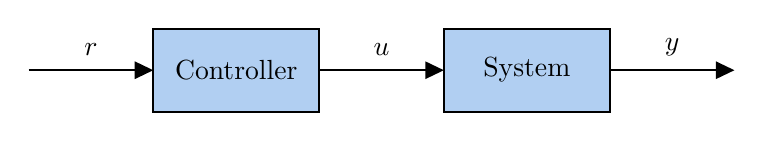
\begin{tikzpicture}[x=0.75pt,y=0.75pt,yscale=-1,xscale=1]
%uncomment if require: \path (0,300); %set diagram left start at 0, and has height of 300

%Flowchart: Process [id:dp0065268414857613255] 
\draw  [fill={rgb, 255:red, 74; green, 144; blue, 226 }  ,fill opacity=0.43 ] (200,110) -- (280,110) -- (280,150) -- (200,150) -- cycle ;
%Flowchart: Process [id:dp7235317018344584] 
\draw  [fill={rgb, 255:red, 74; green, 144; blue, 226 }  ,fill opacity=0.43 ] (340,110) -- (420,110) -- (420,150) -- (340,150) -- cycle ;
%Straight Lines [id:da7470075652158954] 
\draw    (280,130) -- (337,130) ;
\draw [shift={(340,130)}, rotate = 180] [fill={rgb, 255:red, 0; green, 0; blue, 0 }  ][line width=0.08]  [draw opacity=0] (8.93,-4.29) -- (0,0) -- (8.93,4.29) -- cycle    ;
%Straight Lines [id:da5872746694536481] 
\draw    (420,130) -- (477,130) ;
\draw [shift={(480,130)}, rotate = 180] [fill={rgb, 255:red, 0; green, 0; blue, 0 }  ][line width=0.08]  [draw opacity=0] (8.93,-4.29) -- (0,0) -- (8.93,4.29) -- cycle    ;
%Straight Lines [id:da149066055633855] 
\draw    (140,130) -- (197,130) ;
\draw [shift={(200,130)}, rotate = 180] [fill={rgb, 255:red, 0; green, 0; blue, 0 }  ][line width=0.08]  [draw opacity=0] (8.93,-4.29) -- (0,0) -- (8.93,4.29) -- cycle    ;

% Text Node
\draw (240,130) node   [align=left] {Controller};
% Text Node
\draw (380,130) node   [align=left] {System};
% Text Node
\draw (170,124.6) node [anchor=south] [inner sep=0.75pt]    {$r$};
% Text Node
\draw (310,124.6) node [anchor=south] [inner sep=0.75pt]    {$u$};
% Text Node
\draw (450,124.6) node [anchor=south] [inner sep=0.75pt]    {$y$};


\end{tikzpicture}

    \caption{Open Loop Control System}
    \label{fig:Open Loop Controller}
\end{figure}

The image shown in \autoref{fig:Open Loop Controller} is what we call a \textit{block diagram}. It is a diagrammatic representation of how the system behaves. We have some input $r$, which we may call the reference input. In the example of the toaster, this input $r$ is like turning the knob to the desired level. This input feeds into the \textit{controller}, which is something that converts this input into something usable. In our toaster, it converts that mechanical rotation into some electrical signal that the toaster can use to heat our bread. After being converted, this output from the controller is called $u$, the actuating signal. 

This actuating signal, $u$, can then be input into the system. We feed the electric signal, $u$, through some strands of metal in the toaster, which heat up. The system in this case is whatever electronics and physical mechanisms convert this input into the physical heating of the toaster. Once it's done toasting, we have a finished product, $y$, which is our toast.

We can see a very obvious problem with open-loop design -- it cannot correct any errors the system may have. This is perfectly adequate for cooking your toast, but not something as precise as guiding a rocket!
\subsubsection{Closed-Loop Control}
We can alleviate the problems of the open-loop system by introducing \textit{feedback} into the system. The introduction of feedback allows us to check the behavior of the system and make any corrections. We can achieve feedback by implementing a \textit{sensor} which can make determinations about the current state of the system. An example of a closed loop system is shown in \autoref{fig:Closed Loop Controller}.

\begin{figure}[ht]
    \centering

    

\tikzset{every picture/.style={line width=0.75pt}} %set default line width to 0.75pt        

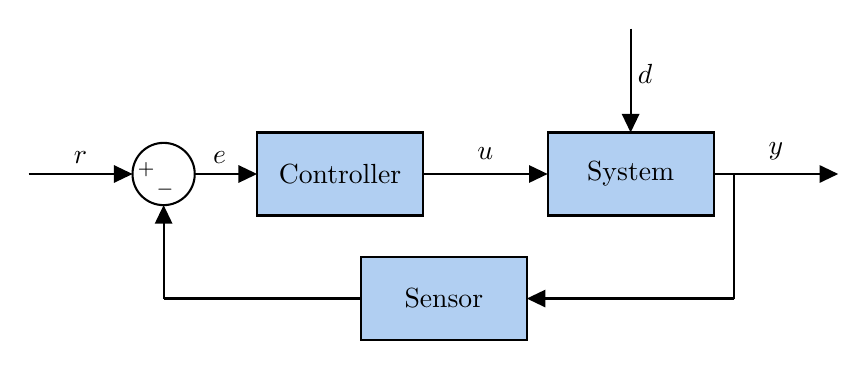
\begin{tikzpicture}[x=0.75pt,y=0.75pt,yscale=-1,xscale=1]
%uncomment if require: \path (0,300); %set diagram left start at 0, and has height of 300

%Flowchart: Process [id:dp5781069900824202] 
\draw  [fill={rgb, 255:red, 74; green, 144; blue, 226 }  ,fill opacity=0.43 ] (220,130) -- (300,130) -- (300,170) -- (220,170) -- cycle ;
%Flowchart: Process [id:dp3913914758716749] 
\draw  [fill={rgb, 255:red, 74; green, 144; blue, 226 }  ,fill opacity=0.43 ] (360,130) -- (440,130) -- (440,170) -- (360,170) -- cycle ;
%Straight Lines [id:da9870933503335829] 
\draw    (300,150) -- (357,150) ;
\draw [shift={(360,150)}, rotate = 180] [fill={rgb, 255:red, 0; green, 0; blue, 0 }  ][line width=0.08]  [draw opacity=0] (8.93,-4.29) -- (0,0) -- (8.93,4.29) -- cycle    ;
%Straight Lines [id:da8934035450659235] 
\draw    (440,150) -- (497,150) ;
\draw [shift={(500,150)}, rotate = 180] [fill={rgb, 255:red, 0; green, 0; blue, 0 }  ][line width=0.08]  [draw opacity=0] (8.93,-4.29) -- (0,0) -- (8.93,4.29) -- cycle    ;
%Straight Lines [id:da9745554219227698] 
\draw    (110,150) -- (157,150) ;
\draw [shift={(160,150)}, rotate = 180] [fill={rgb, 255:red, 0; green, 0; blue, 0 }  ][line width=0.08]  [draw opacity=0] (8.93,-4.29) -- (0,0) -- (8.93,4.29) -- cycle    ;
%Flowchart: Process [id:dp028475583879581712] 
\draw  [fill={rgb, 255:red, 74; green, 144; blue, 226 }  ,fill opacity=0.43 ] (270,190) -- (350,190) -- (350,230) -- (270,230) -- cycle ;
%Straight Lines [id:da9728235475278715] 
\draw    (450,150) -- (450,210) ;
%Straight Lines [id:da38660703137622787] 
\draw    (450,210) -- (353,210) ;
\draw [shift={(350,210)}, rotate = 360] [fill={rgb, 255:red, 0; green, 0; blue, 0 }  ][line width=0.08]  [draw opacity=0] (8.93,-4.29) -- (0,0) -- (8.93,4.29) -- cycle    ;
%Shape: Circle [id:dp9386966287156486] 
\draw   (160,150) .. controls (160,141.72) and (166.72,135) .. (175,135) .. controls (183.28,135) and (190,141.72) .. (190,150) .. controls (190,158.28) and (183.28,165) .. (175,165) .. controls (166.72,165) and (160,158.28) .. (160,150) -- cycle ;
%Straight Lines [id:da5785406425189984] 
\draw    (175,210) -- (175,168) ;
\draw [shift={(175,165)}, rotate = 90] [fill={rgb, 255:red, 0; green, 0; blue, 0 }  ][line width=0.08]  [draw opacity=0] (8.93,-4.29) -- (0,0) -- (8.93,4.29) -- cycle    ;
%Straight Lines [id:da8174390393137155] 
\draw    (175,210) -- (270,210) ;
%Straight Lines [id:da5394055506067064] 
\draw    (190,150) -- (217,150) ;
\draw [shift={(220,150)}, rotate = 180] [fill={rgb, 255:red, 0; green, 0; blue, 0 }  ][line width=0.08]  [draw opacity=0] (8.93,-4.29) -- (0,0) -- (8.93,4.29) -- cycle    ;
%Straight Lines [id:da027328232541036224] 
\draw    (400,80) -- (400,127) ;
\draw [shift={(400,130)}, rotate = 270] [fill={rgb, 255:red, 0; green, 0; blue, 0 }  ][line width=0.08]  [draw opacity=0] (8.93,-4.29) -- (0,0) -- (8.93,4.29) -- cycle    ;

% Text Node
\draw (260,150) node   [align=left] {Controller};
% Text Node
\draw (400,150) node   [align=left] {System};
% Text Node
\draw (135,146.6) node [anchor=south] [inner sep=0.75pt]    {$r$};
% Text Node
\draw (330,144.6) node [anchor=south] [inner sep=0.75pt]    {$u$};
% Text Node
\draw (470,144.6) node [anchor=south] [inner sep=0.75pt]    {$y$};
% Text Node
\draw (310,210) node   [align=left] {Sensor};
% Text Node
\draw (161,148) node [anchor=west] [inner sep=0.75pt]  [font=\scriptsize]  {$+$};
% Text Node
\draw (170,157.5) node [anchor=west] [inner sep=0.75pt]  [font=\scriptsize]  {$-$};
% Text Node
\draw (402,102) node [anchor=west] [inner sep=0.75pt]    {$d$};
% Text Node
\draw (202,146.6) node [anchor=south] [inner sep=0.75pt]    {$e$};


\end{tikzpicture}


    \caption{Closed-Loop Control System}
    \label{fig:Closed Loop Controller}
\end{figure}

This diagram indicates the key components of a closed-loop system. We have many components from the open-loop system again, such as the controller and the system. Now, we add a sensor, which senses the final output $y$. The $+/-$ element takes the difference between the input $r$ and the sensor measurement to generate an error, $e$. This error is now what feeds the controller. Typically, the goal of the closed-loop system is to configure the controller such that the error eventually goes to zero. In a well defined system, we can reduce this error to zero even when the system is subjected to disturbances, $d$!

We can take the analogy of walking through your house to demonstrate the key difference with the closed-loop system. Now, you have your eyes (the sensor) to aid you in walking through your house. This makes it much easier and you can account for disturbance events. If your cat walks across the hall, you can make some adjustment to your path. We can see that closed-loop systems are preferable in most complex applications. As a result, the rest of this book will put its emphasis on closed-loop (sometimes called feedback control) system design.

\subsection{Features of Closed-Loop Systems}
There are still several further distinctions that can be made about control systems. We can classify systems as either \textit{linear} or \textit{non-linear}, and \textit{time invariant} or \textit{time varying}.

A system can have either of these attributes. For example, a system can be time varying, but also linear. A system cannot, however, be both linear and non-linear, as these are mutually exclusive. In the next section we will discuss exactly what we mean by each of these terms.

\subsubsection{Linear Systems}
Linear systems are best thought of in the following way: If we have one solution to the equation, and another solution to the equation, we can add them and get another valid solution. That is to say, in the more technical language, that a linear mapping exists. In control theory and other engineering and physics disciplines, this property is often referred to as \textit{superposition}.

Linear systems are useful for mathematics because they are easily solved. We have an immense number of tools at our disposal to solve linear equations. As a result, much of the theory of control systems is built around linear systems. A more formal definition of linear systems is to come.

\subsubsection{Nonlinear Systems}
Of course, there are systems that are also non-linear. In fact, almost everything in the real world is non-linear to some extent. Any time we have a characteristic of a system that is a function of, say, $x^2$, $\sin x$, or $xy$, we have a nonlinearity. More specifically, they are non-linear in one of the variables of the state, like $x$.

Nonlinearities are everywhere in the real world. Even the beloved mass-spring system, if we were to construct it in the real world, would be somewhat non-linear. Luckily, there are ways we can tackle these nonlinearities. One such way is to understand the non-linearity with a manifold structure, as we do in \autoref{chap:lie theory}. There are other approaches too which can allow us to approximate solutions to non-linear systems. The typical workflow for a non-linear system is to make a simplification to linearize the system in some way. For example, we may take the first derivative at some point to find a linearization of the function. From here, we can apply the tools that we develop for linear systems to help us formulate a control scheme.

Often, the next step after linearization is to simulate the full non-linear dynamics with this control scheme acting on it. If we have chosen an appropriate linearization, the system will remain close to this linear region, even though our system itself is non-linear. Otherwise, we go back and make modifications to the control scheme to make it work with the nonlinear system.

The last step is to deploy the control system on the real-world system. If our modeling of the real world system is adequate, our control scheme should work appropriately. For some applications however, such as control systems for high-powered rockets, there are many aspects of the simulation that are hard to account for and the control system design is very strict. Therefore, more modification is often required at this point. We may either choose to incorporate more realistic system attributes in our model, or choose a different control strategy.

The key thing to note is that non-linear systems very often do not have closed-form solutions. As a result, we apply our knowledge of linear systems to help us in our initial development of a control system. The engineering challenge is to find a control system which works for the true nonlinear system, is cost effective, and is versatile to whatever disturbances or changes we expect. This is quite a tall order, but we will spend the rest of this book building up the theory and using practical examples to do this! Luckily, our knowledge of dynamics that we've built up along the way will help us immensely.

\subsubsection{Time Invariant Systems}
Time invariant systems are the next distinction to discuss. Time invariance is quite simple -- the system properties do not change over time. Of course, the state of the system will evolve over time, otherwise nothing would happen at all. By time invariant, we mean that characteristics that we define as traits of the system itself are constant. This will be easier to see when we develop our mathematical models, but we effectively mean that criteria such as the `System' in \autoref{fig:Closed Loop Controller} do not change at all over time. In a simple system like a mass spring damper, this would mean that $k$, $c$, and $m$ are constant over time.

\subsubsection{Time Varying Systems}
Time varying systems are those systems which do have elements that vary with time. For example, in our rocket, the mass changes as the fuel is expelled out of the back of the rocket. This is a feature that is dependent on time, so we say that our system is time variant.

Typically, time variant systems are not much harder to implement in code, as we can approximate these systems as being time invariant at every time step when we consider small enough $\Delta t$ increments. However, they may be much harder to solve by hand. As such, most of the systems that we consider in the theory section will be time invariant.

In fact, most of the theory of classical control theory is based around these simple linear time invariant (\gls{lti}) systems. We can even further simplify this by considering control systems which are \gls{siso}. This will be the foundation with which we start our exploration of control theory. Before we do so, however, we must explore the tools which we will use in analyzing linear control systems.

\chapter{The Laplace Domain}\label{chap:laplace domain}

Now that we have established a basic view of control theory, we must develop the appropriate mathematical tools to understand the behavior of \gls{lti} systems. The most useful tool for us in doing so is the \gls{laplace transform}.

The \gls{laplace transform} is an integral transform, much like the \textit{Fourier Transform}. We find the \gls{laplace transform} of particular importance for its applications in solving linear differential equations. The \gls{laplace transform} is especially useful because it converts a linear differential equation into an algebraic equation. Since we are well versed in solving algebraic equations, we can understand our control system very well in the Laplace domain.

This conversion of a differential equation to an algebraic equation, combined with a bit of practice, is enough to effectively use the \gls{laplace transform}. However, it doesn't give us an appreciation of \textit{what} the \gls{laplace transform} actually is. Here, I want to present an alternative impetus for the \gls{laplace transform} that is often not taught in introductory differential equations, by analyzing the \glspl{eigenfunction} of the derivative operator. I hope this explanation will be useful both to those learning the subject for the first time and to those seeing the subject again. I will admit, however, this explanation will be most useful to those who have at least seen the \gls{laplace transform} before.

I find this explanation especially enlightening on this topic, although others may prefer the more conventional approach to this topic. As such, I have included some resources that cover the \gls{laplace transform} in the more conventional manner. If you are already familiar with the \gls{laplace transform}, you may skip to \autoref{chap: lti}.

\section{Eigenfunctions}

Before\footnote{Section 1 and 2 of this chapter may be skipped without loss of continuity.} we start our discussion of \glspl{eigenfunction}, we should remember what eigenvalues and eigenvectors in linear algebra are. I find the etymology of this word especially useful in this case. Eigen, in German, is a word meaning `self' or `own'. So, any time we see something, such as an eigenvalue or \gls{eigenfunction}, it is a quantity for which it in some way produces itself. From linear algebra, we are familiar with the following equation:
$$A\xi=\lambda\xi$$
Where we denote an eigenvector by $\xi$ and an eigenvalue by $\lambda$. Note that $A\in\mathbb{C}^{n\times n}$ and $\xi\in\mathbb{C}^n$ in general. From this equation, we can see that the eigenvectors are the special vectors that when multiplied with $A$ are only scaled by some factor $\lambda$. A standard course in linear algebra should have covered this idea in detail for finite dimensional spaces. Let's keep this in mind as we extend this concept from vectors to functions. The two situations are very analogous.

\Glspl{eigenfunction} are in essence, the building blocks of the solutions for equations, much like eigenvectors are the building blocks of matrices. When we have a linear operator, such as an integral or derivative, there must exist a function that when acted upon by this operator, is unchanged by the operator aside from being scaled. This is precisely what we mean when we define something as an \gls{eigenfunction}.  We define the eigenfunction mathematically as:
$$Df=\lambda f$$
Where $D$ is some operator\endnote{In the future, we take $D$ to be the total derivative. However, $D$ in this context may represent any linear operator. For our uses in this book it is fine to consider $D$ as the total derivative operator exclusively.}, $f$ is a function, and $\lambda$ is an eigenvalue. Notice the similarity between the equation for an eigenfunction and the eigenvectors.  We have replaced the eigenvector with a function, and the matrix $A$ by an operator, $D$.

There is a subtle nuance, which is important enough to briefly discuss. When we talk about an eigenfunction or a linear operator, what we are really doing is defining an \textit{abstract} vector space.\footnote{Consider watching \cite{3blue1brown_abstract_2016} for more information.} As it turns out, an eigenfunction is exactly the same as an eigenvector, but existing in an infinite dimensional space. When we define a function, $f(x)$, we may think of it as a vector where each element of the vector is corresponding to an output of $f(x)$. In such a way, we may encode all of the information of $f(x)$ in a vector. This vector will have an infinite length, but it will encode all the information of $f(x)$ exactly. This is illustrated in \autoref{fig:func as vector}.

\begin{figure}[ht]
    \centering


\tikzset{every picture/.style={line width=0.75pt}} %set default line width to 0.75pt        

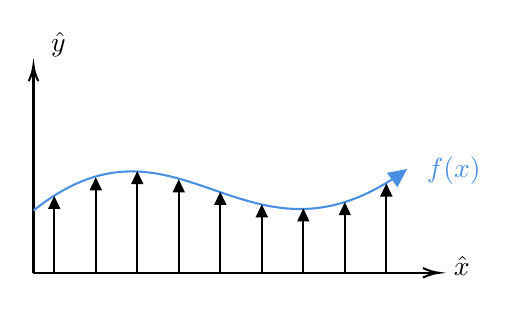
\begin{tikzpicture}[x=0.75pt,y=0.75pt,yscale=-1,xscale=1]
%uncomment if require: \path (0,300); %set diagram left start at 0, and has height of 300

%Straight Lines [id:da5140671078626177] 
\draw    (230,150) -- (230,52) ;
\draw [shift={(230,50)}, rotate = 90] [color={rgb, 255:red, 0; green, 0; blue, 0 }  ][line width=0.75]    (7.65,-2.3) .. controls (4.86,-0.97) and (2.31,-0.21) .. (0,0) .. controls (2.31,0.21) and (4.86,0.98) .. (7.65,2.3)   ;
%Straight Lines [id:da2891080037896999] 
\draw    (230,150) -- (423.3,150) ;
\draw [shift={(425.3,150)}, rotate = 180] [color={rgb, 255:red, 0; green, 0; blue, 0 }  ][line width=0.75]    (7.65,-2.3) .. controls (4.86,-0.97) and (2.31,-0.21) .. (0,0) .. controls (2.31,0.21) and (4.86,0.98) .. (7.65,2.3)   ;
%Curve Lines [id:da8389634124830535] 
\draw [color={rgb, 255:red, 74; green, 144; blue, 226 }  ,draw opacity=1 ]   (230,120) .. controls (299.88,64.26) and (331.95,155.18) .. (407.69,101.67) ;
\draw [shift={(410,100)}, rotate = 143.62] [fill={rgb, 255:red, 74; green, 144; blue, 226 }  ,fill opacity=1 ][line width=0.08]  [draw opacity=0] (8.93,-4.29) -- (0,0) -- (8.93,4.29) -- cycle    ;
%Straight Lines [id:da15406660458008248] 
\draw    (240,150) -- (240,116) ;
\draw [shift={(240,113)}, rotate = 90] [fill={rgb, 255:red, 0; green, 0; blue, 0 }  ][line width=0.08]  [draw opacity=0] (6.25,-3) -- (0,0) -- (6.25,3) -- cycle    ;
%Straight Lines [id:da9921690821184993] 
\draw    (260,150) -- (260,107) ;
\draw [shift={(260,104)}, rotate = 90] [fill={rgb, 255:red, 0; green, 0; blue, 0 }  ][line width=0.08]  [draw opacity=0] (6.25,-3) -- (0,0) -- (6.25,3) -- cycle    ;
%Straight Lines [id:da8140815730656824] 
\draw    (280,150) -- (280,104) ;
\draw [shift={(280,101)}, rotate = 90] [fill={rgb, 255:red, 0; green, 0; blue, 0 }  ][line width=0.08]  [draw opacity=0] (6.25,-3) -- (0,0) -- (6.25,3) -- cycle    ;
%Straight Lines [id:da8300844429249556] 
\draw    (300,150) -- (300,108) ;
\draw [shift={(300,105)}, rotate = 90] [fill={rgb, 255:red, 0; green, 0; blue, 0 }  ][line width=0.08]  [draw opacity=0] (6.25,-3) -- (0,0) -- (6.25,3) -- cycle    ;
%Straight Lines [id:da8758764492171939] 
\draw    (320,150) -- (320,114) ;
\draw [shift={(320,111)}, rotate = 90] [fill={rgb, 255:red, 0; green, 0; blue, 0 }  ][line width=0.08]  [draw opacity=0] (6.25,-3) -- (0,0) -- (6.25,3) -- cycle    ;
%Straight Lines [id:da3715469807264673] 
\draw    (340,150) -- (340,120) ;
\draw [shift={(340,117)}, rotate = 90] [fill={rgb, 255:red, 0; green, 0; blue, 0 }  ][line width=0.08]  [draw opacity=0] (6.25,-3) -- (0,0) -- (6.25,3) -- cycle    ;
%Straight Lines [id:da021202010953294104] 
\draw    (360,150) -- (360,122) ;
\draw [shift={(360,119)}, rotate = 90] [fill={rgb, 255:red, 0; green, 0; blue, 0 }  ][line width=0.08]  [draw opacity=0] (6.25,-3) -- (0,0) -- (6.25,3) -- cycle    ;
%Straight Lines [id:da8134401356974554] 
\draw    (380,150) -- (380,119) ;
\draw [shift={(380,116)}, rotate = 90] [fill={rgb, 255:red, 0; green, 0; blue, 0 }  ][line width=0.08]  [draw opacity=0] (6.25,-3) -- (0,0) -- (6.25,3) -- cycle    ;
%Straight Lines [id:da05780942926193877] 
\draw    (400,150) -- (400,110) ;
\draw [shift={(400,107)}, rotate = 90] [fill={rgb, 255:red, 0; green, 0; blue, 0 }  ][line width=0.08]  [draw opacity=0] (6.25,-3) -- (0,0) -- (6.25,3) -- cycle    ;

% Text Node
\draw (431,140.4) node [anchor=north west][inner sep=0.75pt]    {$\hat{x}$};
% Text Node
\draw (237,32.4) node [anchor=north west][inner sep=0.75pt]    {$\hat{y}$};
% Text Node
\draw (418,92.4) node [anchor=north west][inner sep=0.75pt]  [color={rgb, 255:red, 74; green, 144; blue, 226 }  ,opacity=1 ]  {$f( x)$};


\end{tikzpicture}

    \caption{Function represented by a vector}
    \label{fig:func as vector}
\end{figure}

In this illustration, only a few of the infinitely many values of this vector are shown. In the limit where this vector is infinite-dimensional, we can perfectly represent this function as a vector. Axiomatically, we can see that this vector representation is perfectly valid. After all, all of the axioms of a vector space hold true for functions\endnote{In this example, we take $f,g,h$ to be vectors and $a,b$ to be scalars}:
\begin{enumerate}
    \item $f+(g+h)=(f+g)+h$ (Associativity)
    \item $f+g=g+f$ (Commutativity)
    \item There is a vector $0$ such that $0+f=f \ \forall f$ (Additive identity)
    \item For all $f$ there exist $-f$ such that $f+(-f)=0$ (Additive inverse)
    \item $a(bf)=(ab)f$ (Scalar multiplication)
    \item $1f=f$ (Multiplicative identity)
    \item $a(f+g)=af+ag$ (Distributivity of scalar)
    \item $(a+b)f=af+bf$ (Distributivity of vector)
\end{enumerate}
You may go through and check that each of these properties hold for a function like $f(x)$ from $\mathbb{R}\rightarrow\mathbb{R}$. It suffices to say that we can represent functions equally well using vectors. 

This is the reason that we can define \glspl{eigenfunction} and eigenvalues. It is precisely because this situation is no different than our standard linear algebra. Physicists and engineers often choose to use different vocabulary to describe this space of functions, but the mathematical ideas transfer well. Some of these new definitions are included in \autoref{tab:lin alg to func}:

\begin{table}
    \centering
\caption{Standard definitions in linear algebra when applied to functions}
\label{tab:lin alg to func}
    \begin{tabular}{cc}\toprule
         \textbf{Linear Algebra}&  \textbf{Functions}\\\midrule
         Eigenvalue&  Eigenvalue\\
         Eigenvector&  Eigenfunction\\
 Linear Transformation&Linear Operator\\
 Dot product&Inner Product\\ \bottomrule
    \end{tabular}
    
    
\end{table}

Having understood some of the nuances of the case of functions, let's return to our study of differential equations, in which we are concerned with finding our eigenfunction for the derivative operator. In ordinary differential equations, we use the total derivative to describe all of our equations. As such, finding the eigenfunction for this total derivative is especially useful for us -- and is what will lead us directly to an understanding of the Laplace transform.

It is with this context that we investigate the exponential function, $e^{ax}$, which we find useful for exactly this property. More precisely, we want to solve the eigenvalue system $Df=\lambda f$, where we denote the differentiation operator $\frac{d}{dx}\equiv D$.\endnote{This notation for the derivative is the \textit{Eulerian} notation, if you are curious. Interestingly, Euler did not use this notation, and it was invented by Arbogast.} We can see that, plugging in $e^{ax}$ for $f$, we have this exact property:
$$De^{ax}=ae^{ax}$$
So we have our eigenfunction, $e^{ax}$, which produces an eigenvalue $a$. So, we have found a function $e^{ax}$ which satisfies this condition for the total derivative (our linear operator). If you are curious why this particular function is the eigenfunction of the derivative, read \autoref{sec:derivation of exp} of the Appendix.

Now, we want to use this useful property on equations that are not purely exponential equations. We can once again lean on our experience with linear algebra to understand how we may do this. In linear algebra, we may understand how similar two vectors are with the dot product. If our two vectors are aligned, the dot product returns a value of $1$, and returns a value of $0$ when the two vectors are orthogonal to each other.\endnote{We enforce the condition that both vectors are normalized so that the dot product returns 1.}

We can come up with an analogous operation when using functions instead of vectors. Formally, we call this operation a \textit{projection} of these functions. Our goal, then, is to project an arbitrary function on to the exponential functions that we have created. This will tell us how `similar' such a function is to our exponential functions. The question then arises: How can we project functions on to each other? That is the function of the inner product, which we discuss next.

\section{Inner Product Spaces}\label{sec: inner prod}
To perform this projection, we must first define some new terminology and mathematical understanding. In mathematics, we often have a simple case which we want to generally extend. The same is true here, which will motivate our discussion of inner products.

We start with the standard definition of projection in a finite-dimensional vector space. We consider two vectors, both existing in $\mathbb{R}^2$ space, which is shown in \autoref{fig:2d vec}.

\begin{figure}[ht]
    \centering
    

\tikzset{every picture/.style={line width=0.75pt}} %set default line width to 0.75pt        

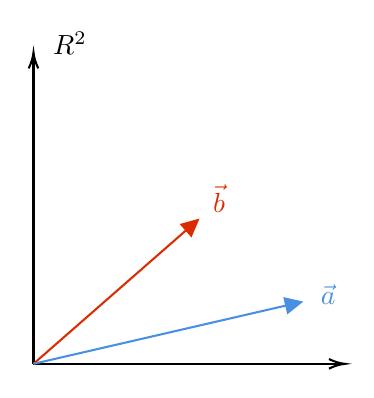
\begin{tikzpicture}[x=0.75pt,y=0.75pt,yscale=-1,xscale=1]
%uncomment if require: \path (0,300); %set diagram left start at 0, and has height of 300

%Straight Lines [id:da1402308417777972] 
\draw    (250,230) -- (250,82) ;
\draw [shift={(250,80)}, rotate = 90] [color={rgb, 255:red, 0; green, 0; blue, 0 }  ][line width=0.75]    (7.65,-2.3) .. controls (4.86,-0.97) and (2.31,-0.21) .. (0,0) .. controls (2.31,0.21) and (4.86,0.98) .. (7.65,2.3)   ;
%Straight Lines [id:da8323133877657714] 
\draw    (250,230) -- (398,230) ;
\draw [shift={(400,230)}, rotate = 180] [color={rgb, 255:red, 0; green, 0; blue, 0 }  ][line width=0.75]    (7.65,-2.3) .. controls (4.86,-0.97) and (2.31,-0.21) .. (0,0) .. controls (2.31,0.21) and (4.86,0.98) .. (7.65,2.3)   ;
%Straight Lines [id:da984721650125026] 
\draw [color={rgb, 255:red, 218; green, 44; blue, 0 }  ,draw opacity=1 ]   (250,230) -- (327.74,161.98) ;
\draw [shift={(330,160)}, rotate = 138.81] [fill={rgb, 255:red, 218; green, 44; blue, 0 }  ,fill opacity=1 ][line width=0.08]  [draw opacity=0] (8.93,-4.29) -- (0,0) -- (8.93,4.29) -- cycle    ;
%Straight Lines [id:da12678737743098834] 
\draw [color={rgb, 255:red, 74; green, 144; blue, 226 }  ,draw opacity=1 ]   (250,230) -- (377.08,200.67) ;
\draw [shift={(380,200)}, rotate = 167.01] [fill={rgb, 255:red, 74; green, 144; blue, 226 }  ,fill opacity=1 ][line width=0.08]  [draw opacity=0] (8.93,-4.29) -- (0,0) -- (8.93,4.29) -- cycle    ;

% Text Node
\draw (258,68.54) node [anchor=north west][inner sep=0.75pt]    {$\mathbb{R}^{2}$};
% Text Node
\draw (387,190.4) node [anchor=north west][inner sep=0.75pt]  [color={rgb, 255:red, 74; green, 144; blue, 226 }  ,opacity=1 ]  {$\vec{a}$};
% Text Node
\draw (335,142.4) node [anchor=north west][inner sep=0.75pt]  [color={rgb, 255:red, 218; green, 44; blue, 0 }  ,opacity=1 ]  {$\vec{b}$};


\end{tikzpicture}

    \caption{The standard picture of 2-D vectors}
    \label{fig:2d vec}
\end{figure}

If we want to find the component of one vector in the direction of the other vector (that is to say, find the component of $\vec{b}$ in the direction of $\vec{a}$), we use the linear operation of the dot product. This quantity tells us the `similarity' of the two vectors.

We can start with an intuitive definition of the dot product and build up from there. We often see the dot product written out as: $$a\cdot b=|a||b|\cos\theta$$
This definition intuitively matches our `similarity' criteria. If the two vectors have the same angle, they are very `similar', and so the $\cos\theta$ term is 1. However, if the two vectors are oriented $90\degree$ from each other, we see that this term goes to zero, as the vectors are completely dissimilar (orthogonal).

This definition only has a physical meaning to us when we can define an angle between the two vectors $\vec{a}$ and $\vec{b}$. Beyond 3-dimensional space, this concept of an angle between vectors begins to be more unclear (although it is still mathematically valid).

As a result, we often want to use an alternative definition of the dot product. We can formulate such a definition by writing something that is equivalent to the case for two dimensions but that will extend to higher dimensions as well.

We can do this by considering the decomposition of a vector in $\mathbb{R}^2$, which we can then extend to many dimensions. In \autoref{fig:vec decomp}, this is shown for the case of $\mathbb{R}^2$ space.
\begin{figure}[ht]
    \centering




\tikzset{every picture/.style={line width=0.75pt}} %set default line width to 0.75pt        

\begin{tikzpicture}[x=0.75pt,y=0.75pt,yscale=-1,xscale=1]
%uncomment if require: \path (0,300); %set diagram left start at 0, and has height of 300

%Straight Lines [id:da67293580166529] 
\draw    (270,250) -- (270,102) ;
\draw [shift={(270,100)}, rotate = 90] [color={rgb, 255:red, 0; green, 0; blue, 0 }  ][line width=0.75]    (7.65,-2.3) .. controls (4.86,-0.97) and (2.31,-0.21) .. (0,0) .. controls (2.31,0.21) and (4.86,0.98) .. (7.65,2.3)   ;
%Straight Lines [id:da25752973634046794] 
\draw    (270,250) -- (418,250) ;
\draw [shift={(420,250)}, rotate = 180] [color={rgb, 255:red, 0; green, 0; blue, 0 }  ][line width=0.75]    (7.65,-2.3) .. controls (4.86,-0.97) and (2.31,-0.21) .. (0,0) .. controls (2.31,0.21) and (4.86,0.98) .. (7.65,2.3)   ;
%Straight Lines [id:da4451601467637182] 
\draw  [dash pattern={on 0.84pt off 2.51pt}]  (390,180) -- (390,250) ;
%Straight Lines [id:da2667435734649499] 
\draw  [dash pattern={on 0.84pt off 2.51pt}]  (390,180) -- (270,180) ;
%Straight Lines [id:da16843504883751226] 
\draw [color={rgb, 255:red, 74; green, 144; blue, 226 }  ,draw opacity=1 ]   (270,250) -- (387.41,181.51) ;
\draw [shift={(390,180)}, rotate = 149.74] [fill={rgb, 255:red, 74; green, 144; blue, 226 }  ,fill opacity=1 ][line width=0.08]  [draw opacity=0] (8.93,-4.29) -- (0,0) -- (8.93,4.29) -- cycle    ;

% Text Node
\draw (407,162.4) node [anchor=north west][inner sep=0.75pt]  [color={rgb, 255:red, 74; green, 144; blue, 226 }  ,opacity=1 ]  {$\vec{a}$};
% Text Node
\draw (424,239.4) node [anchor=north west][inner sep=0.75pt]    {$\hat{e}_{1}$};
% Text Node
\draw (244,92.4) node [anchor=north west][inner sep=0.75pt]    {$\hat{e}_{2}$};
% Text Node
\draw (278,88.54) node [anchor=north west][inner sep=0.75pt]    {$\mathbb{R}^{n}$};
% Text Node
\draw (381,252.4) node [anchor=north west][inner sep=0.75pt]  [color={rgb, 255:red, 74; green, 144; blue, 226 }  ,opacity=1 ]  {$a_{1}$};
% Text Node
\draw (253,172.4) node [anchor=north west][inner sep=0.75pt]  [color={rgb, 255:red, 74; green, 144; blue, 226 }  ,opacity=1 ]  {$a_{2}$};

\end{tikzpicture}

    \caption{Vector decomposition in 2-D}
    \label{fig:vec decomp}
\end{figure}

We can apply the our definition of the dot product to this vector to understand it's decomposition. By taking the dot product between $\vec{a}$  and $\hat{e}_1$, we get a resulting element $a_1$ in the direction of $\hat{e}_1$. This component $a_1$ is also orthogonal to $\hat{e}_2$,  so the dot product between $a_1$ and $\hat{e}_2$ is zero! We can use the same reasoning to write $a_2$ solely in terms of $\hat{e}_2$.

In fact, when we use an orthonormal basis, we will always be able to decompose a vector of dimension $n$ into the dot products with each axis in $\mathbb{R}^n$ space. We can express this for an arbitrary $n$-dimensional space as:
$$\sum_{i=1}^n{a_i\hat{e}_i}$$
Of course these properties are fairly obvious and we have seen vector decomposition since kindergarten. However, it is worth covering this concept again as we will extend this idea and make it more abstract.

Now that we know how this relationship works for a vector and the basis, we can take the dot product between two vectors, $\vec{a}$ and $\vec{b}$, which gives $\vec{a}\cdot\vec{b}$.

\begin{figure}[ht]
    \centering

\tikzset{every picture/.style={line width=0.75pt}} %set default line width to 0.75pt        

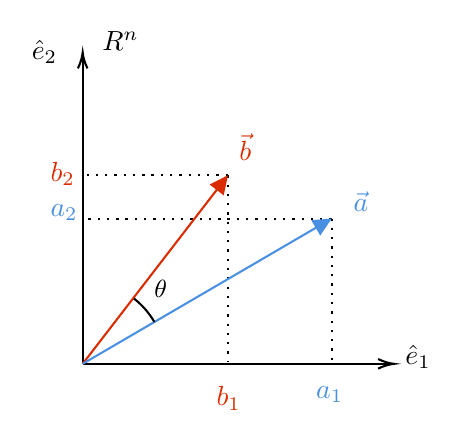
\begin{tikzpicture}[x=0.75pt,y=0.75pt,yscale=-1,xscale=1]
%uncomment if require: \path (0,300); %set diagram left start at 0, and has height of 300

%Straight Lines [id:da07194338650536147] 
\draw    (270,220.86) -- (270,72.86) ;
\draw [shift={(270,70.86)}, rotate = 90] [color={rgb, 255:red, 0; green, 0; blue, 0 }  ][line width=0.75]    (7.65,-2.3) .. controls (4.86,-0.97) and (2.31,-0.21) .. (0,0) .. controls (2.31,0.21) and (4.86,0.98) .. (7.65,2.3)   ;
%Straight Lines [id:da8965708304392496] 
\draw    (270,220.86) -- (418,220.86) ;
\draw [shift={(420,220.86)}, rotate = 180] [color={rgb, 255:red, 0; green, 0; blue, 0 }  ][line width=0.75]    (7.65,-2.3) .. controls (4.86,-0.97) and (2.31,-0.21) .. (0,0) .. controls (2.31,0.21) and (4.86,0.98) .. (7.65,2.3)   ;
%Straight Lines [id:da9421113913029678] 
\draw  [dash pattern={on 0.84pt off 2.51pt}]  (390,150.86) -- (390,220.86) ;
%Straight Lines [id:da7944597894464402] 
\draw  [dash pattern={on 0.84pt off 2.51pt}]  (390,150.86) -- (270,150.86) ;
%Straight Lines [id:da3683558397635107] 
\draw  [dash pattern={on 0.84pt off 2.51pt}]  (340,130) -- (340,220) ;
%Straight Lines [id:da5891702614671979] 
\draw  [dash pattern={on 0.84pt off 2.51pt}]  (340,130) -- (270,130) ;
%Straight Lines [id:da5322994190102411] 
\draw [color={rgb, 255:red, 218; green, 44; blue, 0 }  ,draw opacity=1 ]   (270,220.86) -- (338.17,132.38) ;
\draw [shift={(340,130)}, rotate = 127.61] [fill={rgb, 255:red, 218; green, 44; blue, 0 }  ,fill opacity=1 ][line width=0.08]  [draw opacity=0] (8.93,-4.29) -- (0,0) -- (8.93,4.29) -- cycle    ;
%Straight Lines [id:da19322918869231698] 
\draw [color={rgb, 255:red, 74; green, 144; blue, 226 }  ,draw opacity=1 ]   (270,220.86) -- (387.41,152.37) ;
\draw [shift={(390,150.86)}, rotate = 149.74] [fill={rgb, 255:red, 74; green, 144; blue, 226 }  ,fill opacity=1 ][line width=0.08]  [draw opacity=0] (8.93,-4.29) -- (0,0) -- (8.93,4.29) -- cycle    ;
%Shape: Arc [id:dp9279619891884023] 
\draw  [draw opacity=0] (294.74,189.42) .. controls (298.67,192.52) and (302,196.33) .. (304.54,200.67) -- (270,220.86) -- cycle ; \draw   (294.74,189.42) .. controls (298.67,192.52) and (302,196.33) .. (304.54,200.67) ;  

% Text Node
\draw (399,136.4) node [anchor=north west][inner sep=0.75pt]  [color={rgb, 255:red, 74; green, 144; blue, 226 }  ,opacity=1 ]  {$\vec{a}$};
% Text Node
\draw (424,210.26) node [anchor=north west][inner sep=0.75pt]    {$\hat{e}_{1}$};
% Text Node
\draw (244,63.26) node [anchor=north west][inner sep=0.75pt]    {$\hat{e}_{2}$};
% Text Node
\draw (278,59.4) node [anchor=north west][inner sep=0.75pt]    {$\mathbb{R}^{n}$};
% Text Node
\draw (344,108.4) node [anchor=north west][inner sep=0.75pt]  [color={rgb, 255:red, 218; green, 44; blue, 0 }  ,opacity=1 ]  {$\vec{b}$};
% Text Node
\draw (381,230.4) node [anchor=north west][inner sep=0.75pt]  [color={rgb, 255:red, 74; green, 144; blue, 226 }  ,opacity=1 ]  {$a_{1}$};
% Text Node
\draw (253,142.4) node [anchor=north west][inner sep=0.75pt]  [color={rgb, 255:red, 74; green, 144; blue, 226 }  ,opacity=1 ]  {$a_{2}$};
% Text Node
\draw (333,230.4) node [anchor=north west][inner sep=0.75pt]  [color={rgb, 255:red, 218; green, 44; blue, 0 }  ,opacity=1 ]  {$b_{1}$};
% Text Node
\draw (253,122.4) node [anchor=north west][inner sep=0.75pt]  [color={rgb, 255:red, 218; green, 44; blue, 0 }  ,opacity=1 ]  {$b_{2}$};
% Text Node
\draw (303,178.83) node [anchor=north west][inner sep=0.75pt]  [font=\small]  {$\theta $};


\end{tikzpicture}


    \caption{The link between the algebraic and geometric dot product}
    \label{fig:geometric dot}
\end{figure}
We can see in \autoref{fig:geometric dot} that we have the geometric representation, $\vec{a}\cdot\vec{b}=|a||b|\cos\theta$. We can equivalently write the algebraic representation, using the fact that we can decompose the vectors into their components in the basis directions for both $\vec{a}$ and $\vec{b}$. Now that both are in the same plane, we can multiply the components in a way we are familiar with, the simple $a*b=ab$. Doing so gives us:
$$\vec{a}\cdot\vec{b}=a_1\hat{e}_1*b_1\hat{e}_1+a_1\hat{e}_1*b_2\hat{e}_2+a_2\hat{e}_2*b_1\hat{e}_1+a_2\hat{e}_2*b_2\hat{e}_2$$
Using the independence of the basis from before, we can cancel any terms which have $\hat{e}_1*\hat{e}_2$, since we know these two to be orthogonal! Additionally we know that $\hat{e}_1*\hat{e}_1=1$ since $\hat{e}_1$ has a unit length. Thus our dot product is simply 
$$\vec{a}\cdot\vec{b}=a_1b_1+a_2b_2$$
We can generalize this statement past the two dimensional space by realizing that any two indices that are not-equal will be non orthogonal. That is, $\hat{e}_i*\hat{e}_j=0$ for $i\neq j$. We can then define the dot product of two vectors in a finite $n$-dimensional space generally as:
$$\vec{a}\cdot \vec{b}=\sum_{k=1}^{n}{a_kb_k}$$
We can equivalently represent these thoughts more rigorously with the following mathematical argument. Our original sum is the following:
$$\vec{a}\cdot \vec{b}=\sum_{j=1}^n\sum_{k=1}^{n}{a_jb_k}\delta_{jk}$$
The orthogonality of the basis introduces the $\delta_{jk}$ term (Kronecker-delta). Because the Kronecker delta is 1 only when $j=k$, we can reduce the double sum to the single sum:
$$\vec{a}\cdot \vec{b}=\sum_{k=1}^{n}{a_kb_k}$$

As we have seen earlier, we can also express this sum more compactly if we consider $\vec{a}$ and $\vec{b}$ to be column vectors. We can write the multiplication as:
$$\vec{a}\cdot \vec{b}=\vec{a}^T\vec{b}$$
So far, our discussion has been only on the dot product. However, the inner product, as we have seen, is the extension of this idea to functions. When we deal with functions, we need to consider that we may have complex numbers, and the fact that our vectors have an infinite number of components. Let us consider those possibilities now.

\subsubsection{Extension to Complex Numbers}
We find complex functions to be quite useful in the study of control theory, where analysis in the complex domain is very common. In other words, we are extending our domain from $\mathbb{R}^n$ to $\mathbb{C}^n$.

A natural way to do this is by considering the equivalent operation of the transpose for complex numbers, which we call the conjugate transpose. Unfortunately, there are many different notations for this, some including $\bar{A}$, $A^*$, and $A^{\dagger}$. Here, I will use $A^*$ notation which has also been used in Volume II. Using this notation, we can denote the inner product of two complex-valued vectors as:
$$\vec{a}\cdot\vec{b}=\vec{a}^*\vec{b}$$
We can equivalently write this in the summation notation. For single complex numbers, the conventional notation is to write the conjugate as $\bar{b}$. Some write the conjugate as $b^*$, but to avoid confusing this with the matrix operation of the conjugate transpose, I will use the bar notation instead. As we can see, nothing about the inner product changes aside from the fact that we must take the \textit{conjugate} of $b_k$ now, so that:
$$\vec{a}\cdot \vec{b}=\sum_{k=0}^{n}{a_k\bar{b}_k}$$
We define the conjugate of $b$ to have the same real part, $\sigma$, but the imaginary part of the function is negated.
\begin{equation}
    \begin{split}
        b&=\sigma+i\omega\\
        \bar{b}&=\sigma-i\omega
    \end{split}
\end{equation}

\subsection{Creating Inner Product Spaces}

% draw the function in terms of the vectors

Now, we can make a generalization to arrive at the inner product. Let's remember that we have a continuous function, $f(x)$. We can encode $f(x)$ as a vector by taking a measurement of the value of $f(x)$ at each input $x$. However, we must extend our current definition to account for the fact that this vector has an infinite length. We might try to do this by extending our sum out to infinity. Now our $a$ and $b$ are functions of $t$ since they are continuous in time. We may write this as something like:
$$a(t)\cdot b(t)=\sum_{k=0}^{\infty}{a_kb_k}$$
Since we are summing to infinity, things can get out of control now! If the values of $a$ and $b$ never go to zero, then the sum will go off to infinity and be undefined. This is no good for us -- we want to work with functions that have finite values. There are a few things that we can do here. The first is impose that $a$ and $b$ must tend to zero as they approach $\infty$. This condition is not true for a general function, but if we think about functions describing real phenomenon, this is often the case.\endnote{This is commonly supposed in physics.} When we interpret the dot product as an energy, it makes sense to suppose that it must be bounded.

Another option is that we may consider a finite interval, $\tau$, which means that we are less restrictive in the selection of functions. So long as a function does not have a value that approaches $\infty$ over the range of $\tau$, then this condition is satisfied. We can mathematically define this condition:
$$\int_0^\tau{|f(t)|^2}dt<\infty$$
Mathematicians define a space with these properties as a Lebesgue space. A Lebesgue space may be defined in many ways, but we will stick to a quite simple definition. We will only consider Euclidean geometry, where lengths are given by the familiar Pythagorean distance: $\sqrt{{x_1}^2+{x_2}^2+\dots {x_n}^2}$. We call this way of measuring distance a 2-norm. For a general p-norm, we can define the distance as:
$$||x||_p=\left({|x_1|}^p+{|x_2|}^p+\dots+{|x_n|}^p\right)^{\frac{1}{p}}$$
For now, we are only concerned with the case where $p=2$, which we call the 2-norm (also called the Euclidean norm). Sometimes we use other norms in fields like optimal control, so it is good to introduce the general concept here.

All of this formalism leads us to the final important result, which we call the $L^2$ space -- $L$ for Lebesgue and $2$ for the 2-norm. In an $L^2$ space defined over the range $(0,\tau)$, we write the inner product as\endnote{I should note that the addition of $\frac{1}{\tau}$ is not \textit{strictly} necessary to make this an inner product. Instead, it is there as a `normalization' factor in our inner product such that it will return a magnitude of $1$ in the expected circumstances (orthonormal functions) whose norms are unity.}:
\begin{equation}\label{eq:inner product}
    a(t)\cdot b(t)=\frac{1}{\tau}\int_0^\tau{a(t)\overline{b(t)}}dt
\end{equation}
Before we move on to the \gls{laplace transform}, let's take a moment to remember what we have just achieved with \eqautoref{eq:inner product}. This equation is telling us the similarity between functions $a$ and $b$. If $a(t)$ is really `similar' to $b(t)$, this inner product should give us a value that is `similar' to $a(t)$. If $a(t)$ are orthogonal functions, this will give us 0. The result of this is that we can understand how close an arbitrary function is to say, $\sin{t}$, using this equation.

\begin{exercise}[Inner Product]
Consider an $L^2$ space over the range $(0,2\pi)$. Find the inner product of the following functions:
\begin{enumerate}
    \item $\sin{t}\cdot\cos{t}$
    \item $t\cdot t^2$
    \item $e^{it}\cdot e^{2it}$
\end{enumerate}
\end{exercise}

Before we move on, let's take the intuition we've developed about inner products and formalize it. Here, we've described a specific $L^2(0,\tau)$ inner product space. In general, an inner product space needs to satisfy the following criteria:
\begin{enumerate}
    \item Conjugate Symmetry: $a\cdot b=\overline{b\cdot a}$. When $a,b$ are real, then $a\cdot b={b\cdot a}$
    \item Linearity: $(ax+by)\cdot z=a(x\cdot z)+b(y\cdot z)$
    \item Positivity: $x\cdot x \ge 0$. $x\cdot x =0$ iff $x=0$.
\end{enumerate}

If you want other examples of inner product spaces, see \autoref{sec:inner prod ex} in the Appendix. Inner product spaces are crucial in defining the Fourier transform, Legendre polynomials, and many other tools in math, physics, and engineering.

\section{The Laplace Transform}
We can now return to the example of the exponential functions, $e^{at}$, which were the eigenfunction of the derivative. We have previously seen that these exponential functions are key in describing the solutions to linear differential equations. To further extend this definition, we can consider values of $a$ which are complex. We generally denote such complex values as $s$, which gives us the general function: $e^{st}$. This function contains all of the possible behaviors of a \textit{linear} differential equation.\endnote{Any deviation from a linear system can produce results not in the span of $e^{st}$. We can only apply the Laplace transform to linear systems.} 

We can convince ourselves of this fact pretty easily. Let's consider a general linear differential equation with constant coefficients. This will look like:
$$a_0y+a_1\dot{y}+a_2\ddot{y}+\cdots+a_ny^{(n)}=0$$
We suppose that the solution to this equation is comprised of only exponential functions (which is what we want to show). We can plug in exponential function $y=e^{\alpha t}$ and see that:
$$a_0e^{\alpha t}+a_1\alpha e^{\alpha t}+a_2\alpha^2 e^{\alpha t}+\cdots+a_n\alpha^n e^{\alpha t}=0$$
We can factor out $e^{\alpha t}$ and see that our equation must satisfy:
$$a_0+a_1\alpha +a_2\alpha^2+\cdots+a_n\alpha^n =0$$
Thus, the solutions to this equation are the roots of this polynomial equation which has $n$ roots. Assuming distinct roots, they will form a basis $\left\{e^{\alpha_1t},e^{\alpha_2t},\cdots,e^{\alpha_nt}\right\}$ for the solution space.\endnote{Otherwise, we will see multiplication by $t$ in the solution for repeated roots. The \gls{laplace transform} will still handle such cases.} Thus, the exponential function governs the behavior of the whole class of \gls{lti} differential equations. 

\subsubsection{Deriving the Laplace Transform}
Let's remember the important property of linear differential equations -- we may add solutions together in superposition. Therefore, if we can construct all the possible solutions to a linear ordinary differential equation using $e^{st}$, we may express the solution to any differential equation using the inner product of our function with $e^{st}$ over $L^2[0,\infty)$.\endnote{I may note that $e^{st}\notin L^2[0,\infty)$ in some cases, because $e^{st}$ diverges to infinity. Thus, this inner product is not strictly correct in the functional-analytic sense in the same way as the Fourier transform. We may still think of the projection onto exponential functions in much the same way. However, we restrict our domain to piecewise-continuous functions with $|f(t)|\le Me^{\alpha t}$ with the condition that $M>0$ and $\alpha\in\mathbb{R}$. We rarely encounter any function in control theory which does not meet these conditions but exception is worth noting. }

So, we can project our function onto the basis vectors defined by $e^{st}$ to understand our differential equation. Remembering that we must conjugate $e^{st}$ when we take the inner product (giving us $e^{-st}$), we have the \gls{laplace transform}:
\begin{gather}\label{eq:laplace transform}
    \color{boxBlue}\boxed{\color{black}\mathscr{L}\{f(t)\}=\int_0^\infty{f(t)e^{-st}}}\\
    \color{boxBlue}\mathrm{Laplace \ Transform}
\end{gather}
Whatever we do with the \gls{laplace transform} from now on, always try to carry the intuition as well. This transform tells us how similar a function is to a certain complex exponential!

The \gls{laplace transform} will prove extraordinarily useful for analyzing \gls{lti} systems. We may refer to the \gls{laplace transform} of a function $f(t)$ by $\mathscr{L}\left\{f(t)\right\}$. We generally denote this \gls{laplace transform} in shorthand as $$\mathscr{L}\left\{f(t)\right\}\Rightarrow F(s)$$
It is typical to denote the transformation both by a chance of variable from $t$ to $s$ as well as from a lowercase function, such as $f$, to an upper case one, $F$. I note that the \gls{laplace transform} has transformed our function from one in the time domain, $t$, to one in the $s$-domain! This $s$-domain has some very unique properties which come as a result of intentionally choosing the exponential function as our basis. The properties important to our study of control theory will be explored in the following section.
\subsection{Properties of the Laplace Transform}\label{sec:properties of laplace transform}

There are many properties of the \gls{laplace transform}. We are not concerned with deriving all of these, although most are quite easy to prove simply by plugging them into \eqautoref{eq:laplace transform}. A list of the commonly used \glspl{laplace transform} can be found at \cite{dawkins_differential_nodate}. The derivations for most of these are just manipulations of the integral, so I will not cover them unless they are particulary insightful.

Here, I want to cover a few of the most useful properties for understanding control theory. Of course, all of the transforms are useful in their own right, and many of them come up in problems. For that reason, I recommend the reader is at least comfortable with manipulating equations in the $s$-domain, and converting back and forth. This skill just comes with practice. I have included a few practice problems at the end of this section if you want to practice these transformations.

That being said, let us begin by covering some of the most useful \glspl{laplace transform}, which are listed below:
\begin{itemize}
    \item Exponential function
    \item Sinusoid
    \item Step Function
    \item Delta Function
    \item Derivatives
    \item Integrals
\end{itemize}
\subsubsection{Exponential Functions}
Exponential functions, as previously mentioned, are quite common in differential equations and control theory. For this reason, we start with these. Finding the \gls{laplace transform} for the exponential function is quite easy, actually! We consider the general exponential function $e^{at}$, and plug into \eqautoref{eq:laplace transform}:
$$\int_0^\infty{e^{at}e^{-st}}dt$$
We can combine the two exponentials in this equation to get:
$$\int_0^\infty{e^{t(a-s)}}dt$$
Upon the integration of this equation, we have
$$\left .\frac{e^{t(a-s)}}{a-s}\right|_0^\infty=\lim_{t\rightarrow\infty}\frac{e^{(a-s)t}}{a-s}-\frac{1}{a-s}$$
In the case that $\Re s>a$, then the first term evaluates to $0$ as the exponential has a negative exponent. We are thus left with:
$$\mathscr{L}\left\{e^{at}\right\}=\frac{1}{s-a}$$
Since we know that exponentials with positive values for $a$ diverge to infinity for positive $t$, and those with negative values for $a$ converge to zero, we can find the stability of a system based on the sign of $s-a$! When the sign is negative, $s-2$ -- for example -- the exponential is unstable. When it is positive, $s+2$ for example, it is stable. We will further explore these concepts, but it is something worth noting now!

\subsubsection{Sinusoids}
From the exponentials, we are only a short step from the sinusoidal functions. Since the two functions are closely related, it is quite simple to develop appropriate transforms of the sinusoids using the Euler equation:
$$e^{ix}=\cos x+i\sin x$$
\begin{exercise}[Laplace Transform of $\sin$ and $\cos$]
    Using the Euler equation above, prove that the $\sin(at)$ function has a \gls{laplace transform}:
$$\mathscr{L}\left\{\sin(at)\right\}=\frac{a}{s^2+a^2}$$
and that $\cos(at)$ function has a \gls{laplace transform}:
$$\mathscr{L}\left\{\cos(at)\right\}=\frac{s}{s^2+a^2}$$
\end{exercise}

It is interested to note, that if we consider values of $s$ that are purely imaginary, that is $s=i\omega$, these formulas simplify a bit. For $\sin$, we have the following:
$$\mathscr{L}\{\sin(at)\}=\frac{a}{a^2-\omega^2}$$
When we plug in a frequency, $\omega=a$, that is the same as the frequency of the sine wave, we divide by zero! This division by zero is what we call a \textit{pole} in the complex plane. We typically represent these with an `x' marker in the complex plane, as shown in \autoref{fig: sine wave}.

\begin{figure}[ht]
    \centering


\tikzset{every picture/.style={line width=0.75pt}} %set default line width to 0.75pt        

\begin{tikzpicture}[x=0.75pt,y=0.75pt,yscale=-1,xscale=1]
%uncomment if require: \path (0,300); %set diagram left start at 0, and has height of 300

%Straight Lines [id:da6143378059913305] 
\draw    (330,60) -- (330,220) ;
%Straight Lines [id:da32627873590921797] 
\draw    (410,140) -- (250,140) ;
%Straight Lines [id:da37253286393851626] 
\draw [color={rgb, 255:red, 218; green, 44; blue, 0 }  ,draw opacity=1 ]   (330,100) ;
\draw [shift={(330,100)}, rotate = 45] [color={rgb, 255:red, 218; green, 44; blue, 0 }  ,draw opacity=1 ][line width=0.75]    (-5.59,0) -- (5.59,0)(0,5.59) -- (0,-5.59)   ;
%Straight Lines [id:da11664231471930675] 
\draw [color={rgb, 255:red, 218; green, 44; blue, 0 }  ,draw opacity=1 ]   (330,180) ;
\draw [shift={(330,180)}, rotate = 45] [color={rgb, 255:red, 218; green, 44; blue, 0 }  ,draw opacity=1 ][line width=0.75]    (-5.59,0) -- (5.59,0)(0,5.59) -- (0,-5.59)   ;

% Text Node
\draw (348,52.4) node [anchor=north west][inner sep=0.75pt]    {$\mathbb{C}$};
% Text Node
\draw (340,92) node [anchor=north west][inner sep=0.75pt]    {$a$};
% Text Node
\draw (323,40.4) node [anchor=north west][inner sep=0.75pt]    {$\omega $};
% Text Node
\draw (414,134) node [anchor=north west][inner sep=0.75pt]    {$\sigma $};
% Text Node
\draw (338,172) node [anchor=north west][inner sep=0.75pt]    {$-a$};

\end{tikzpicture}
    
    \caption{Complex Plane Representation of Sine Wave}
    \label{fig: sine wave}
\end{figure}
This plot, which we call a pole-zero plot, tells us a lot of information about the system. Here, it tells us that the function $\sin(at)$ has poles that are purely imaginary. That means that they will oscillate, without decaying or growing, forever. The same is true of cosine, since the denominator of the equation is the same.

\begin{exercise}
    We have stated that the $\sin$ and $\cos$ functions have poles which are purely imaginary. We know that we can represent a function in the Laplace domain as the addition of $e^{st}$ components. Prove that we can represent $\sin{at}$ and $\cos{at}$ using the Euler identity: $e^{i\theta}=\cos\theta+i\sin\theta$ to get:
    $$\cos{at}=\frac{1}{2}\left(e^{iat}+e^{-iat}\right)$$   $$\sin{at}=\frac{1}{2i}\left(e^{iat}-e^{-iat}\right)$$
    and show that the poles are indeed located on the purely imaginary line $\Re=0$ and that these always come in conjugate pairs.
\end{exercise}

\subsubsection{Step Function}
The step function has a value of $0$ until time $t=0$, after which it attains a value of $1$. The unit step function is sometimes denoted with $u(t)$, but since we use $u$ to denote a control input, we will instead denote it $1^+(t)$. This notation is certainly less often used but it is often the case that both the unit step and $u$ as a control input exist in the same equation.

The unit step function can also have a time offset, which is the same as a usual function, where the offset is to the right is given by the value $c$ and the form of the step function is $1^+(t-c)$ or ${1_c}^+(t)$

We can apply the integral transform on ${1_c}^+(t)$, which means that the integral from $0\le t \le c$ will be zero. The \gls{laplace transform} of the step function gives:

$$\mathscr{L}\left\{{1_c}^+(t)\right\}=\frac{e^{-cs}}{s}$$
The unit step function often multiplies other functions as well. The \gls{laplace transform} in this case is given by:
$$\mathscr{L}\left\{{1_c}^+(t)f(t-c)\right\}=e^{-cs}F(s)$$
Or as is more often the case:
$$\mathscr{L}\left\{{1_c}^+(t)f(t)\right\}=e^{-cs}\mathscr{L}\left\{f(t+c)\right\}$$
These equations can easily be derived from the integral expression of the \gls{laplace transform} which has previously been shown.

\subsubsection{Delta Function}
The delta function is not a traditional function, but rather a distribution with all of the power concentrated in one infinitesimal amount of time. The delta function can be thought of as an instantaneous `ring' or impulse which is sent into the system. The function is defined as follows:
\begin{gather}
    \delta(t)=\begin{cases}
        0,\quad t\neq0\\
        \infty,\quad t=0
    \end{cases}
\end{gather}
With an additional condition that the total integral of the function is 1:
$$\int_{-\infty}^{\infty}\delta(t)dt=1$$
Another useful property of the Dirac delta function is that when multiplying with another function, the integral is simply:
$$\int_{-\infty}^{\infty}f(t)\delta(t)dt=f(0)$$
We can use this property to find the \gls{laplace transform} of the Dirac delta function:
$$\int_{-\infty}^{\infty}e^{-st}\delta(t)dt=e^{-0}=1$$
As can be seen, the Dirac delta has the very helpful feature that it acts as a multiplicative identity in the Laplace domain. This property is very useful and will be important later.

Often, we want to define a delta function in which the impulse occurs at a time other than $t=0$. In this case, we often denote this function $\delta_c(t)$ or $\delta(t-c)$. In this case, the total integral of the function must still be equal to 1. However, we now have:
$$\int_{-\infty}^{\infty}f(t)\delta_c(t)dt=f(c)$$
From which it follows that the \gls{laplace transform} of the general Dirac delta is:
$$\int_{-\infty}^{\infty}e^{-st}\delta_c(t)dt=e^{-cs}$$

Notice that the step function is different from the delta function by a factor of $\frac{1}{s}$. We may also notice that integrating over the delta function gives us a step function! This is a clue that this factor of $\frac{1}{s}$ is the equivalent of integration in the Laplace domain. This is a good point to examine differentiation and integration in the Laplace domain.
\subsubsection{Differentiation}
Differentiation was the operation that was our original impetus for the \gls{laplace transform}. It is no surprise, then, that the derivative has quite a clean representation in the Laplace domain. We may start with the definition of the \gls{laplace transform}, as usual:
$$\mathscr{L}\left\{\frac{df}{dt}\right\}=\int_0^\infty{\frac{d}{dt}(fe^{-st})dt}$$
This is a typical case where we use the product rule of integration (otherwise called by-parts integration).
$$\int_0^\infty{\frac{d}{dt}(fe^{-st})dt}=\int_0^\infty\frac{df}{dt}e^{-st}+(-fse^{-st})dt$$
This equation can be rearranged, and the fundamental theorem of calculus applied to give (go through this yourself to verify):
$$\mathscr{L}\left\{\frac{df}{dt}\right\}=sF(s)-f(0)$$
In the case where $f(0)=0$, we have that the derivative simply gives a multiplication by $s$. Turning differentiation into multiplication is one of the key attributes of the \gls{laplace transform}, because it turns a differential equation into an algebraic one.

\subsubsection{Integration}
We have some clue from our previous example that integration should give us a factor of $\frac{1}{s}$ in the Laplace domain. Since integration is the inverse operation of differentation, we may immediately guess that this should be the case. We may verify with the following argument.
$$g(t)=\int_0^tf(\tau)d\tau,\quad g(0)=0$$
From this definition, we can see that $\frac{dg}{dt}=f$. Using the definition of the derivative from before, we have:
$$\mathscr{L}\left\{\frac{dg}{dt}\right\}=s\mathscr{L}\{g(t)\}-g(0)$$
Which gives us 
$$\mathscr{L}\left\{\frac{dg}{dt}\right\}=F(s)$$
Solving the lefthand side to get $G(s)$ gives us another term in $s$ from the derivative. Thus,
$$G(s)=\frac{F(s)}{s}$$

\subsubsection{Frequency Shift Theorem}
When we multiply a function, by $e^{-at}$, we have a special property. We can once again use our definition of the \gls{laplace transform}:
$$\mathscr{L}\{e^{-at}f(t)\}=\int_0^\infty{e^{-(s+a)t}f(t)dt}$$
From this statement it is evident that we may directly replace $u\equiv s+a$ in the integral to get:
$$\mathscr{L}\{e^{-at}f(t)\}=\int_0^\infty{e^{-ut}f(t)dt}=F(u)$$
Which comes directly from our definition of the transform. Plugging in $s+a$ for $u$, we have the property:
\begin{gather}
    \color{blue}\boxed{\color{black}\mathscr{L}\{e^{-at}f(t)\}=F(s+a)}\\
    \color{blue}\text{Frequency Shift Theorem}
    \end{gather}
This frequency shift theorem tells us that an exponential decay in the time domain, $e^{-at}$, is equivalent to a shift by $a$ in the frequency domain. Thus, as we move our poles further to the \textit{left} in the frequency domain, the faster our function decays in the time domain.

As we saw before, we can represent a functions behavior by the location of the poles. When we had a sinusoidal function, we had:
\begin{figure}[ht]
    \centering
    \includesvg[width=\linewidth]{Images/sinFunction2.svg}
    \caption{Poles of a sine wave}
    \label{fig:sin wave poles}
\end{figure}
If we multiply the function with $e^{-0.5t}$, we get a decay in our function over time. We can do this to our $\sin(t)$ function, which gives us the following:
\begin{figure}[ht]
    \centering
     \includesvg[width=\linewidth]{Images/sinFunctionDecay2.svg}
    \caption{Poles of a decaying sine wave}
    \label{fig:decaying sine wave poles}
\end{figure}
As we can see, this new function decays according to the red `envelope' function, $e^{-0.5t}$. The poles of the function have shifted to the \textit{left} now, so that we get the decay in the response. Notice that these poles still come in the conjugate pair, as we saw earlier. However, the $\Re$ component has shifted to the left by $a$.

\subsubsection{Time Shift Theorem}
Similar to the frequency shift theorem, if we have a function that is shifted in the time domain, we have an effect in the frequency domain. We saw this with the delta function, where:
$$\mathscr{L}\{\delta(t)\}=1$$
But, if we shifted the delta function to start at time $c$ (which we denoted as $\delta_c(t)$), then we had:
$$\mathscr{L}\{\delta_c(t)\}=e^{-cs}$$
The time shift theorem tells us that when we have a function $f(t-c)$, representing a shift in the function to the right by $c$ in the time domain, we get a corresponding exponential decay component in the frequency domain:
$$\mathscr{L}\{f(t+c)\}=e^{-cs}F(s)$$
We can see an exact symmetry between this case and the frequency shift case, but we have now changed the role of the time domain and the frequency domain. With this theorem, we have now developed all of the tools of the \gls{laplace transform} which are of considerable use to us.

\subsubsection{Final Value Theorem}
We can sometimes use the Laplace domain to understand the time domain behavior of functions. One very useful tool is the final value theorem, which lets us determine the end behavior of a function as $t\rightarrow \infty$.

\begin{theorem}{Final Value Theorem}
    Given a function in the Laplace domain, $Y(s)$, if all of the poles of $Y(s)$ are in the left half plane\endnote{We will discuss what this means more exactly in the next chapter.}, then
    $$\lim_{t\rightarrow\infty} y(t)=\lim_{s\rightarrow 0}sY(s)$$
\end{theorem}
\begin{proof}\textbf{Proof of Final Value Theorem}\\
Consider a function $y(t)$ and its derivative $y'(t)$. We consider $y(t)$ to be bounded at infinity, continuous, and smooth. We may take the \gls{laplace transform} of the derivative of $y(t)$, which gives:
$$\mathscr{L}\{y'(t)\}=sY(s)-y(0)$$
We take the limit of this \gls{laplace transform} at $s\rightarrow 0$.
$$\lim_{s\rightarrow0}sY(s)-y(0)$$
Which we leave for now. Let's consider the integral definition of $\mathscr{L}\{y'(t)\}$:
$$\mathscr{L}\{y'(t)\}=\int_0^\infty{}e^{-st}y'(t)dt$$
We evaluate the limit as $s\rightarrow0$ for this expression
    $$\mathscr{L}\{y'(t)\}=\lim_{s\rightarrow0}\int_0^\infty{}e^{-st}y'(t)dt=\int_0^\infty{}y'(t)dt$$
    Since this is an improper integral, we take the limit at $t\rightarrow\infty$ to evaluate.
    $$\int_0^\infty{}y'(t)dt=\lim_{t\rightarrow\infty}y(t)-y(0)$$
    We now equate the two expressions:
    $$\lim_{t\rightarrow\infty}y(t)-y(0)=\lim_{s\rightarrow0}sY(s)-y(0)$$
    and find that $y(0)$ cancels from both sides of the equation, leaving us with:
      $$\lim_{t\rightarrow\infty}y(t)=\lim_{s\rightarrow0}sY(s)$$
\end{proof}
\
\subsubsection{Initial Value Theorem}
We can do something similar if we would like to find the initial value of a function. Our theorem looks very similar:

\begin{theorem}{Initial Value Theorem}
    Given a function in the Laplace domain, $Y(s)$, then
    $$\lim_{s\rightarrow\infty} sY(s)=y(0+)$$
\end{theorem}
\begin{exercise}[Initial Value Theorem]
    Prove the initial value theorem using a proof similar to the final value theorem. Hint: consider the integral definition of the \gls{laplace transform}.
\end{exercise}

\begin{exercise}[Laplace Transform Practice]
    Find the Laplace transforms of the following functions (you may use the Laplace tables provided in \cite{dawkins_differential_nodate}). For $2$, use the final value theorem. For $1$ and $3$, use the initial value theorem. Check these against the time domain solutions.
    \begin{enumerate}
        \item $t\sin 4t$
        \item $e^{-t}\cos3t$
        \item $\sinh{3t}$
    \end{enumerate}
\end{exercise}
\subsection{Inverse Laplace Transform}
For classical control theory, it is often the case that almost all of our analysis can be done in the $s$-domain. As a result, the inverse Laplace transform is less useful than the forward transform. However, it is still worth noting briefly.

The inverse Laplace transform allows us to take a function in the $s$-domain and convert it back to the time domain. We represent this as:
$$\mathscr{L}^{-1}\left\{F(s)\right\}\Rightarrow f(t)$$
The solution of this equation looks similar to the \gls{laplace transform}, but involves solving a contour integral:
$$f(t)=\frac{1}{2\pi i}\int_\gamma{F(s)e^{st}ds}$$
In practice, we don't solve for the inverse Laplace transform using this contour integral when solving by hand. Instead, we try to make the equation amenable to being represented as one of the known \glspl{laplace transform}. These methods involve algebraic manipulation to reach one of the known forms of the Laplace transform. When solving by hand, we often employ two powerful methods:  completing the square, and partial fraction decomposition.

\begin{example}[Completing the Square]
    Consider a function in the Laplace domain given by:
    $$F(s)=\frac{4s+5}{s^2+4s+13}$$
    To find the inverse Laplace transform, we complete the square to get the denominator into a form that can be factored:
    $$\frac{4s+5}{(s+2)^2+9}$$
We want to also have this factor of $(s+2)$ present in the numerator, so that we can pull this term out.
 $$\frac{4(s+2)-3}{(s+2)^2+9}$$
 We can split the resulting fraction into two parts, each of which are recognizable components:
  $$\frac{4(s+2)}{(s+2)^2+9}-\frac{3}{(s+2)^2+9}$$
  Using the tables, we recognize the forms of $\sin$ and $\cos$ components multiplied with a frequency shift (resulting in a $e^{-2t}$ component):
  $$f(t)=4e^{-2t}\cos3t-e^{-2t}\sin3t$$
\end{example}

\begin{example}[Partial Fraction Decomposition]
Sometimes, we need some additional algebraic work to convert our answers from the Laplace domain into the time domain. The primary method for doing this is a technique known as partial fraction decomposition. We consider a function which takes the form of a polynomial divided by another polynomial:
$$G(s)=\frac{N(s)}{D(s)}$$
Let's make this example concrete, considering the following polynomial:
$$G(s)=\frac{3s+5}{s^2+5s+6}$$
Our first step is to rewrite the denominator in a factorized form. For $D(s)=s^2+5s+6$, it is apparent that we can factor this into two first order components, leaving us with:
$$G(s)=\frac{3s+5}{(s+2)(s+3)}$$
Our goal is to make this equation amenable to a form which we can easily find the inverse Laplace transform of. If we could separate this equation into two fractions of the $(s+2)$ and $(s+3)$ terms, we would have a solution with exponential components. Therefore, we want an equation of that form:
$$\frac{A}{s+2}+\frac{B}{s+3}=\frac{3s+5}{(s+2)(s+3)}$$
We can readily multiply each side by $(s+2)(s+3)$, which gives us an equation where $A$ and $B$ are readily solved:
$$A(s+3)+B(s+2)=3s+5$$
We may substitute values of $s$ into this equation to solve for these values. Using $s=-3$, we may solve for $B$:
$$B(-3+2)=3(-3)+5\rightarrow B=4$$
Following a similar procedure, we solve for $A$ to get $A=-1$.
Thus, we have a decomposed fraction which is mathematically equivalent to our original equation:
$$\frac{4}{s+3}-\frac{1}{s+2}=\frac{3s+5}{(s+2)(s+3)}$$
We can use the left side of this equation and take the inverse Laplace transform to get:
$$g(t)=4e^{-3t}-e^{-2t}$$
\end{example}

\subsubsection{Further Notes on Partial Fraction Decomposition}
When performing partial fraction decomposition, there are a few other rules which we should keep in find. First, we often have terms in the denominator with repeated roots. We must decompose these differently. Consider the function:
$$G(s)=\frac{3s}{(s+1)(s+2)^2}$$
To decompose this fraction, we \textit{must} consider the terms $(s+2)$ and $(s+2)^2$ as two separate factors. We do this because it is possible that our decomposed fraction requires both a term in $(s+2)$ and $(s+2)^2$ to satisfy the equality. We write such a partial fraction as:
$$\frac{A}{s+1}+\frac{B}{s+2}+\frac{C}{(s+2)^2}=\frac{3s}{(s+1)(s+2)^2}$$
It is of course possible that some of these coefficients turn out to be zero.
\begin{exercise}[Partial fractions with repeated roots]
    Solve the above example, finding the inverse Laplace transform of:
    $$G(s)=\frac{3s}{(s+1)(s+2)^2}$$
\end{exercise}
As a last note, we sometimes have equations that lead to irreducible quadratic factors. For example, we sometimes have a system like:
$$G(s)=\frac{3+s}{s^3-2s}$$
We may factor out the $s$ in the denominator, to arrive at the following:
$$G(s)=\frac{3+s}{s(s^2-2)}$$
From here, we make no further simplification, since there exist no rational factorization of $s^2-2$. When we try to find the representation of this function using partial fractions, we must keep this term $s^2-2$ as a quadratic. For quadratic terms, our partial fraction decomposition appears like:
$$\frac{A}{s}+\frac{Bs+C}{s^2-2}=\frac{3+s}{s(s^2-2)}$$

\subsection{Computational Tools for Laplace and Inverse Laplace Transform}

Sometimes the expressions for the \gls{laplace transform} and its inverse can be difficult to compute by hand. We can use MATLAB with symbolic toolbox or SymPy in Python.

\subsubsection{Using MATLAB}
To compute the \gls{laplace transform} in MATLAB, we use symbolic variables. To compute the \gls{laplace transform} of $\sin(t)$, we do:

\begin{matlabscript}{}
syms t

laplace(sin(t))
\end{matlabscript}

If we input this into a MATLAB live script, it will output a LaTeX formatted answer in the output:
$$\texttt{ans}=\frac{1}{s^2+1}$$

We may also type in differential equations with the symbolic toolbox. For the differential equation $\ddot{x}=3$, we input:
\begin{matlabscript}{}
syms t x(t)

eqn = diff(x,t,2) == 3

laplace(eqn)
\end{matlabscript}
Which produces the output:
$$s^2 \,\mathrm{laplace}\left(x\left(t\right),t,s\right)-{\left({{\left(\frac{\partial }{\partial t}\;x\left(t\right)\right)}\left|\right.}_{t=0} \right)}-s\,x\left(0\right)=\frac{3}{s}$$
This output is slightly verbose, but it can be simplified if we recognize $\mathrm{laplace}\left(x\left(t\right),t,s\right)=X(s)$.

We have a similar command for the inverse \gls{laplace transform}.
\begin{matlabscript}{}
syms s

ilaplace(1/(s^2+s))
\end{matlabscript}
Again, this outputs a LaTeX formatted output when using a livescript:
$$\texttt{ans}=1-{\mathrm{e}}^{-t}$$

\subsubsection{Using Python}
In Python, we can do similar things using the SymPy package. This package will also output LaTeX formatted results with the proper setup. We often use interactive python for such examples. For the \gls{laplace transform}, we can use a live notebook with the following code:
\begin{pythonscript}{}
import sympy
sympy.init_printing()

import matplotlib.pyplot as plt
%matplotlib inline

t, s = sympy.symbols('t, s')
a = sympy.symbols('a', real=True, positive=True)

f = sympy.exp(-a*t)

F = sympy.laplace_transform(f, t, s, noconds=True)
F
\end{pythonscript}

This produces the output:
$$\frac{1}{a+s}$$

We can also find the inverse \gls{laplace transform}:
\begin{pythonscript}{}
 sympy.inverse_laplace_transform(F, s, t)
\end{pythonscript}

Which of course returns the original function:
$$e^{-at}\theta(t)$$
Where $\theta(t)$ is the Heaviside function. This is identical to our original output for $t>0$.

Once we have the libraries imported, the two languages are very similar. We may even define shorthand functions to make easier to use and more similar to using MATLAB:
\begin{pythonscript}{}
def laplace(f):
    return sympy.laplace_transform(f, t, s, noconds=True)

def ilaplace(F):
    return sympy.inverse_laplace_transform(F, s, t)
\end{pythonscript}

See \cite{sandrock_3_2018} for more information on using the Laplace transform in Python. This website also contains information on using Python for other controls applications.

\section{Additional Exercises}
\begin{exercise}[Laplace Transform Practice]\label{exer_laplace_practice}
    Find the \gls{laplace transform} for the following functions, assuming initial conditions are zero. Check your answers with the computational methods before checking the solutions in the book.
    \begin{enumerate}
        \item $\ddot{x}+2\dot{x}+3=\delta(t)$
        \item $\dddot{x}+3x=\sin(t)$
        \item $m\ddot{x}+c\dot{x}+kx=u$
        \item $e^{at}\sinh{at}$
    \end{enumerate}
\end{exercise}

\begin{exercise}[Inverse Laplace Transform Practice]
    Find the inverse \gls{laplace transform} for the following functions:
    \begin{enumerate}
        \item $G(s)=\frac{4}{(s-3)(s+2)}$
        \item $F(s)=\frac{6(s+1)}{(s+3)(s+6)}$
    \end{enumerate}
\end{exercise}

\newpage
\printendnotes


\chapter{Linear Time Invariant Systems}\label{chap: lti}

\begin{chapquote}{Richard Feynman}
    Finally, we make some remarks on why linear systems are so important. The answer is simple: because we can solve them! So most of the time we solve linear problems. Second (and most important), it turns out that the fundamental laws of physics are often linear. The Maxwell equations for the laws of electricity are linear, for example. The great laws of quantum mechanics turn out, so far as we know, to be linear equations. That is why we spend so much time on linear equations: because if we understand linear equations, we are ready, in principle, to understand a lot of things.
\end{chapquote}

\Gls{lti} systems are the basis for most of classical control theory. It is prudent to start our discussion of control theory with such systems. As we have seen, our Laplace transform is only mathematically true in the case of an \gls{lti} system. These systems will be the basis of almost every control scheme that we describe. Since we can find exact solutions to \gls{lti} systems, we can extend the theories that we study here in many other types of control systems, whether they are non-linear or time varying.

Before we get started, let's take a moment to mathematically describe what we mean by a linear system. We already have a rough idea -- that linear systems can have solutions added together. 

A linear system is \textit{not} an equation of form $y=mx+b$. Instead, what we mean when we have a linear system is that the differential equation itself is linear. A linear differential equation is one in which we can represent our state derivative, $\bm{\dot{x}}$, in terms of its components, $\bm{x}$. Put succinctly, a linear system (without inputs) is one which has the representation
$$\bm{\dot{x}}=A\bm{x}$$
where $A$ is a matrix of scalar coefficients. When our system is linear, it implies that we can add different solutions together to acquire another valid solution. This is a property we call \textit{superposition}.

\begin{example}[Linear system example]\label{ex: linear system}
    Consider a system which is governed by the differential equation
    $$\ddot{x}+2\dot{x}+3x=0$$
To determine if this system is linear, we should check if its amenable to the form $\bm{\dot{x}}=A\bm{x}$. We may start by doing a reduction of order:
\begin{gather}
    y=\dot{x}\\
    \dot{y}=-2y-3x
\end{gather}
From here, it is easy to see that we can write the system in a linear form, since each equation is a first order ODE.
$$\begin{bmatrix}
    \dot{x}\\
    \dot{y}\end{bmatrix}=\begin{bmatrix}
        0&1\\-3&-2    \end{bmatrix}\begin{bmatrix}
            x\\y
        \end{bmatrix}$$
\end{example}

For the moment, we won't concern ourselves with writing our systems as a matrix. This form, known as the \textit{state space} representation, will become important in modern control, but for now it's just a tool that we can use to determine if our system is linear. Let's see how a non-linear system is different and why we can't write it this way.

\begin{example}[Non-linear system]
Consider our system to be
$$\ddot{x}+2x^2+\sin(x)=0$$
Let's try and follow the same methodology as before:
\begin{gather}
    y=\dot{x}\\
    \dot{y}=-2x^2+\sin{x}
\end{gather}
We don't have any derivatives higher than first order, but putting this into a matrix representation is problematic. There is no possible way that we can arrive at $x^2$ or $\sin{x}$ by multiplying $x$ and $y$ with scalar values. So, we must say that this system is non-linear.

The important characteristic is if the differential equation itself has terms which are linear. The \textit{solution} of the differential equation, of course, can be very non-linear, and often will be.
\end{example}
\begin{exercise}[Classify Differential Equations]
To practice with linear systems, determine if the following equations are linear or not:
\begin{enumerate}
    \item $\dot{x}=2x+\sin{3}$
    \item $\dddot{x}+3x=4$
    \item $\dot{x}+4x^2=0$
    \item $x+\tan{x}=0$
\end{enumerate}
\end{exercise}

Although this state space representation is useful, what we will actually start with is using the \gls{laplace transform} to define our system. Such a description allows us to create what is known as the \gls{transfer function} representation. As it turns out, anything we can represent with a \gls{transfer function} must also be linear (and also time invariant in the cases we study). Remember, our Laplace transform is only valid for linear differential equations, so anything we represent in that way will automatically satisfy linearity. This is a very useful property for us. For classical control, we'll focus our efforts on this transfer function representation.

\section{Transfer Functions}
A \gls{transfer function} is a tool that is used in linear control theory to gain an understanding of the input-output relationship of a system. Given a certain input, the transfer function will tell us what the output will be. Let's come up with our definition right at the beginning. The transfer function is the relationship between our input and output, given by the output divided by the input. If we call our transfer function $G$, the input $U$, and the output $Y$, the transfer function is:
$$G(s)=\frac{Y(s)}{U(s)}$$
We can immediately see the use of a transfer function with an example. If we want to go from an input $R(s)$ to an output $Y(s)$, we can use an intermediate \gls{transfer function} $G(s)$, so that the relationship is:
$$R(s)G(s)=Y(s)$$
Notice that we desire this relationship to be a simple multiplication. In the time domain, however, the relationship of the input and the output is quite complicated. To illustrate this complication, we can consider a simple system like a mass spring damper.
\begin{figure}[ht]
    \centering

\includesvg[width=\linewidth]{Images/MSD Time History.svg}

    \caption{Mass Spring Damper Time History}
    \label{fig:msd solution}
\end{figure}

The time history of the oscillation is shown on the right of \autoref{fig:msd solution}. If we want to know the transfer function at time $A$, it is quite hard to do! We would need information about all of the dynamics leading up to that event to understand the current system dynamics at point $A$. That is, even if we can measure the position at $A$, we don't have any information about the velocity or acceleration unless we have already been watching the system.

To construct a mathematical description of the system, we want to understand the input-output relationship of the force and the displacement of the mass. We describe the force input as $u(t)$ and the displacement output as $y(t)$. We should look for some intermediate function, $g(t)$, which maps $u(t)$ to $y(t)$. We can write this relationship as:
$$u(t)*g(t)=y(t)$$
To figure out what this relationship should be, we should start by considering the simple case of the delta function. When a delta function is input, the output of the system for all future times can be measured. Conceptually, we can think of hitting the system with a hammer and seeing what happens in the subsequent time. For a typical system, there will be some oscillation that dies out over time, as shown in \autoref{fig:deltaFunc}.
\begin{figure}[ht]
    \centering
     \includesvg[width=.85\linewidth]{Images/DeltaFunction.svg}
    \caption{Delta Function}
    \label{fig:deltaFunc}
\end{figure}
Let's consider this response due to our impulse $\delta(t)$ to be called $g(t)$. This function $g(t)$ gets a special name -- this is the \textit{impulse response} of the system. It is what we get when we give the system some initial kick and watch it's natural response.

Now, suppose we have a new delta function, which occurs at time $t=1 \ \mathrm{s}$ instead of $t=0 \ \mathrm{s}$. We should expect that the function describing the output should be shifted over by $1 \ \mathrm{s}$ as well.
\begin{figure}[ht]
    \centering
    \includesvg[width=0.75\linewidth]{Images/DeltaFuncOffset.svg}
    \caption{Delta Function with Delay}
    \label{fig:deltaFuncDelay}
\end{figure}
Mathematically, we should expect that the result should look almost identical to $g(t)$, but of course the whole function is shifted over by $1 \text{s}$, so that we have:
$$\delta_1(t)\rightarrow g(t-1)$$

We can think of a general input as consisting of many of these delta functions put together. In that case, our output should be the sum of all of their contributions, as shown in \autoref{fig:deltaFuncSum}.\endnote{This pure addition only works because we have specified the system to be linear. Take a moment to consider how this would break down in the non-linear case.}
\begin{figure}[ht]
    \centering
    \includesvg[width=0.75\linewidth]{Images/DeltaFunctionSum.svg}
    \caption{Sum of Delta Functions}
    \label{fig:deltaFuncSum}
\end{figure}
Mathematically, our total output (which we designate $y(t)$), should be the sum of all these $\delta_c(t)$ contributions. In the example above, this would take the form:
$$y(t)=g(t)*\color{blue}x_0\color{black}+g(t-1)*\color{linkgreen}x_1\color{black}+g(t-2)*\color{red}x_2\color{black}$$
The colors here correspond to the different input $\delta_c(t)$ functions multiplied by some constant to give each one a different height. 

In this general case, we can express this combination as the sum of each of the input functions. We may now consider the input as $x=\{x_0,x_1,\cdots,x_n\}$. Think of $x$ as a linear combination of many $\delta_c(t)$ functions, each multiplied by some magnitude to give them a certain magnitude. In this way, we can model any arbitrary signal $x$. Based on our previous result, we can generalize and see that:
$$y(t) = \sum x(\tau)\cdot g(t-\tau)$$
Of course, if we are to consider the fully continuous case, it is natural that each input is separated in time by $d\tau$, and we instead represent with the integral form.
$$y(t) = \int_0^\infty x(\tau)\cdot g(t-\tau)d\tau$$
We define this operation, often denoted as $x(t)*g(t)$ in short, as the \textit{convolution} operation.

\subsubsection{Transfer Functions in the Laplace Domain}
We have seen that the the description of the input-output relationship in the time domain is quite complex. As a result, it is a good idea to try and express this relationship in the Laplace domain instead. One reason why we might think to try this is that the $\delta(t)$ function was surprisingly clean in the Laplace domain. Since our function was composed of many $\delta(t)$ functions, we may get a nice result for the convolution. We can express the convolution with the Laplace integral as
$$\mathscr{L}\{u(t)*g(t)\}=\int_0^\infty{\left(\int_0^\infty{}u(\tau)g(t-\tau)d\tau\right)}e^{-st}dt$$
We can perform a substitution with $\sigma=t-\tau$, which simplifies the integral to:
$$\mathscr{L}\{u(t)*g(t)\}=\int_0^\infty{\left(\int_0^\infty{}u(\tau)g(\sigma)d\tau\right)}e^{-s(\sigma+\tau)}d\sigma$$
Since $\tau$ is a constant, we can see that $dt=d\sigma$. This allows us to separate the integral into two components:
$$\mathscr{L}\{u(t)*g(t)\}=\int_0^\infty g(\sigma)e^{-s\sigma}d\sigma{\int_0^\infty{}u(\tau)e^{-s\tau}}d\tau$$
We can see that these two integrations are simply the integrals for the \gls{laplace transform} of $g$ and $u$! This gives us the very important result that:
\begin{gather}
\color{boxBlue}\boxed{\color{black}\mathscr{L}\{u(t)*g(t)\}=U(s)G(s)}\\
\color{boxBlue}\text{Laplace transform of convolution}
\end{gather}
The result of this is that we can write the input output relationships in the Laplace domain very simply -- it is simply a multiplication. Considering our original function in the time domain. Remember that the convolution is a complex integration:
$$u(t)*g(t)=y(t)$$
We can rewrite this in the Laplace domain simply as:
$$U(s)G(s)=Y(s)$$
Since we have turned this complicated formula of the convolution into multiplication, it is now trivial to find the transfer function, $G(s)$ through simple manipulation of the equation:
$$G(s)=\frac{Y(s)}{U(s)}$$
So, it turns out that we can use the Laplace domain to turn the complicated time domain representation into a simple multiplication. As a result, we will use the \gls{laplace transform} which we have previously developed to understand control systems. It turns complex input-output relations in the time domain into simple multiplication.
\subsubsection{A physical intuition}
Although we have shown the mathematics which show that the convolution reduces to multiplication in the Laplace domain, I find it quite helpful to examine why this holds from a physical point of view.

We can remember from \autoref{sec:properties of laplace transform} that the \gls{laplace transform} gives us quite simple representations of derivatives and integrals as multiplication and division by $s$. As a result, we can quite easily express equations of motion in the Laplace domain. For example, we can consider the \gls{eom} for a mass spring damper:
$$m\ddot{y}(t)+c\dot{y}(t)+ky(t)=u(t)$$
Expressed in the Laplace domain (assuming that the initial conditions are $0$, which is the usual condition for transfer functions):
$$Y(s)\left[ms^2+cs+k\right]=U(s)$$
Solving for the transfer function, we find that:
$$G(s)=\frac{Y(s)}{U(s)}=\frac{1}{ms^2+cs+k}$$
It is in this equation that the insight behind the \gls{laplace transform} can be discovered. It is exactly the \gls{eom} of the system that determines the input and output mapping!

So, we can see that in the Laplace domain, all of the information of the system dynamics is directly captured in the transfer function. We can therefore, know what the position, velocity, or acceleration are for any value $s$. The tradeoff, of course, is that we lose information on the temporal component, $t$, during the transformation. There is no explicit information contained in this transfer function about how the system evolves with $t$. The $s$, however, gives all the relevant information about governing differential equation.

Despite losing some information about the time evolution, we still find it extremely useful to have this `global view' of the function in the Laplace domain. When we need to consider the temporal aspects of the system, we can either revert to the time domain or use some other tools to understand the temporal nature of the transfer function.

\begin{exercise}[Mass Spring Damper Transfer Function]\label{exer_mass_spring_tf}
Consider a mass spring damper system with a force input $u(t)$. The system has a spring constant $k=2$ and $c=3$, and the mass is $1$.
\begin{enumerate}
    \item Write the equation of motion for the system.
    \item Find the transfer function $\frac{Y(s)}{U(s)}$.
    \item Find the state space for the system (use \autoref{ex: linear system} to help if you are stuck)
    \item We will show later that we may get the transfer function from a state space from the following equation $G(s)=C(sI-A)^{-1}B+D$. Consider the matrix found in part 3 to be the $A$ matrix of the system. Letting $D=0$, $B=\begin{bmatrix}
        0&1
    \end{bmatrix}^\top$, $C=\begin{bmatrix}
        1&0
    \end{bmatrix}$, show that this yields the same transfer function as part 2.
\end{enumerate}
\end{exercise}
    

\section{Block Diagrams}
Block diagrams, which have previously been mentioned in our introduction to controls, are especially useful when we introduce transfer functions. Block diagrams allow us to create a visual representation of our transfer function.  We can manipulate block diagrams in a way that allows us to ascertain the transfer function for a whole system or for specific components. As an example, let us consider the open loop transfer function we showed in the introduction, reproduced below in \autoref{fig:Open Loop Controller 2}.

\begin{figure}[ht]
    \centering


\tikzset{every picture/.style={line width=0.75pt}} %set default line width to 0.75pt        

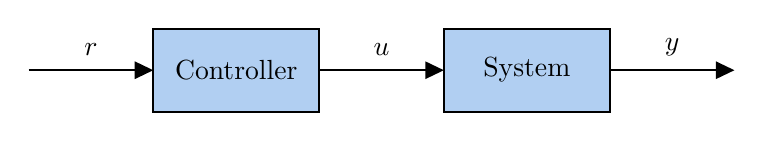
\begin{tikzpicture}[x=0.75pt,y=0.75pt,yscale=-1,xscale=1]
%uncomment if require: \path (0,300); %set diagram left start at 0, and has height of 300

%Flowchart: Process [id:dp0065268414857613255] 
\draw  [fill={rgb, 255:red, 74; green, 144; blue, 226 }  ,fill opacity=0.43 ] (200,110) -- (280,110) -- (280,150) -- (200,150) -- cycle ;
%Flowchart: Process [id:dp7235317018344584] 
\draw  [fill={rgb, 255:red, 74; green, 144; blue, 226 }  ,fill opacity=0.43 ] (340,110) -- (420,110) -- (420,150) -- (340,150) -- cycle ;
%Straight Lines [id:da7470075652158954] 
\draw    (280,130) -- (337,130) ;
\draw [shift={(340,130)}, rotate = 180] [fill={rgb, 255:red, 0; green, 0; blue, 0 }  ][line width=0.08]  [draw opacity=0] (8.93,-4.29) -- (0,0) -- (8.93,4.29) -- cycle    ;
%Straight Lines [id:da5872746694536481] 
\draw    (420,130) -- (477,130) ;
\draw [shift={(480,130)}, rotate = 180] [fill={rgb, 255:red, 0; green, 0; blue, 0 }  ][line width=0.08]  [draw opacity=0] (8.93,-4.29) -- (0,0) -- (8.93,4.29) -- cycle    ;
%Straight Lines [id:da149066055633855] 
\draw    (140,130) -- (197,130) ;
\draw [shift={(200,130)}, rotate = 180] [fill={rgb, 255:red, 0; green, 0; blue, 0 }  ][line width=0.08]  [draw opacity=0] (8.93,-4.29) -- (0,0) -- (8.93,4.29) -- cycle    ;

% Text Node
\draw (240,130) node   [align=left] {Controller};
% Text Node
\draw (380,130) node   [align=left] {System};
% Text Node
\draw (170,124.6) node [anchor=south] [inner sep=0.75pt]    {$r$};
% Text Node
\draw (310,124.6) node [anchor=south] [inner sep=0.75pt]    {$u$};
% Text Node
\draw (450,124.6) node [anchor=south] [inner sep=0.75pt]    {$y$};


\end{tikzpicture}

    \caption{Open Loop Control System}
    \label{fig:Open Loop Controller 2}
\end{figure}

In the Laplace domain, we have shown that the input-output relationship is quite simple and can be represented with multiplication. So, we can replace the controller and the system by transfer functions instead:

\begin{figure}[ht]
    \centering

\tikzset{every picture/.style={line width=0.75pt}} %set default line width to 0.75pt        

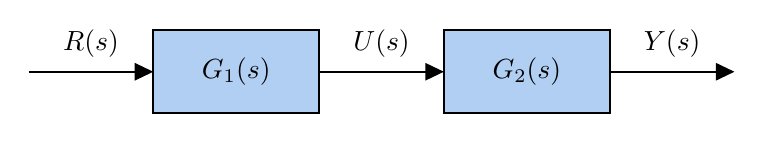
\begin{tikzpicture}[x=0.75pt,y=0.75pt,yscale=-1,xscale=1]
%uncomment if require: \path (0,300); %set diagram left start at 0, and has height of 300

%Flowchart: Process [id:dp22112180414009353] 
\draw  [fill={rgb, 255:red, 74; green, 144; blue, 226 }  ,fill opacity=0.43 ] (220,130) -- (300,130) -- (300,170) -- (220,170) -- cycle ;
%Flowchart: Process [id:dp9940596706792563] 
\draw  [fill={rgb, 255:red, 74; green, 144; blue, 226 }  ,fill opacity=0.43 ] (360,130) -- (440,130) -- (440,170) -- (360,170) -- cycle ;
%Straight Lines [id:da63618583494272] 
\draw    (300,150) -- (357,150) ;
\draw [shift={(360,150)}, rotate = 180] [fill={rgb, 255:red, 0; green, 0; blue, 0 }  ][line width=0.08]  [draw opacity=0] (8.93,-4.29) -- (0,0) -- (8.93,4.29) -- cycle    ;
%Straight Lines [id:da4883479509669909] 
\draw    (440,150) -- (497,150) ;
\draw [shift={(500,150)}, rotate = 180] [fill={rgb, 255:red, 0; green, 0; blue, 0 }  ][line width=0.08]  [draw opacity=0] (8.93,-4.29) -- (0,0) -- (8.93,4.29) -- cycle    ;
%Straight Lines [id:da2671815950803569] 
\draw    (160,150) -- (217,150) ;
\draw [shift={(220,150)}, rotate = 180] [fill={rgb, 255:red, 0; green, 0; blue, 0 }  ][line width=0.08]  [draw opacity=0] (8.93,-4.29) -- (0,0) -- (8.93,4.29) -- cycle    ;

% Text Node
\draw (190,144.6) node [anchor=south] [inner sep=0.75pt]    {$R( s)$};
% Text Node
\draw (330,144.6) node [anchor=south] [inner sep=0.75pt]    {$U( s)$};
% Text Node
\draw (470,144.6) node [anchor=south] [inner sep=0.75pt]    {$Y( s)$};
% Text Node
\draw (260,150) node    {$G_{1}( s)$};
% Text Node
\draw (400,150) node    {$G_{2}( s)$};


\end{tikzpicture}

    \caption{Transfer Function Definition of Open Loop System}
    \label{fig:trans func open loop}
\end{figure}
With these transfer functions, we can quite easily describe how $Y(s)$ varies with the input $R(s)$, just by multiplying the components of the equation! We may write the system as follows\endnote{Note that the transfer function must premultiply the variable that is input into it. This is done so that the transfer function satisfies matrix multiplication rules in the case of transfer function matrices. In the general case, we must be careful of the order.}:
\begin{gather}
    U(s)=G_1(s)R(s)\\
    Y(s)=G_2(s)U(s)
\end{gather}
We can combine these equations to get:
$$Y(s)=G_2(s)G_1(s)R(s)$$
And we may find the transfer function to be:
$$\frac{Y(s)}{R(s)}=G_2(s)G_1(s)$$
And so, we have stumbled upon the first rule of block diagrams: Two transfer functions in series can be multiplied together\endnote{We can derive any block diagram system in this way, no matter how complex. For very complex systems, this algebraic approach is often the simplest. It is worthwhile to discuss some commonly seen block diagram structures to make our lives easier, though.}. Note that the order of multiplication is important! The latest multiplication should be left-multiplied. From here, we may look at the closed-loop system as shown in \autoref{fig:closed loop BD}:\endnote{I have simplified signals and transfer functions by dropping the $s$ (e.g. $R(s)\rightarrow R$). There is no difference other than notational convenience. The time domain and the Laplace domain are often distinguished by the use of lowercase for the time domain, and uppercase letters for the Laplace domain ($r(t) \xrightarrow{\mathscr{L}} R(s)$}

\begin{figure}[ht]
    \centering

\tikzset{every picture/.style={line width=0.75pt}} %set default line width to 0.75pt        

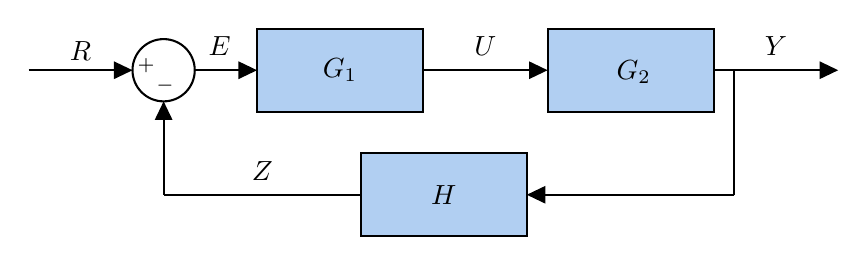
\begin{tikzpicture}[x=0.75pt,y=0.75pt,yscale=-1,xscale=1]
%uncomment if require: \path (0,300); %set diagram left start at 0, and has height of 300

%Flowchart: Process [id:dp5167459085437383] 
\draw  [fill={rgb, 255:red, 74; green, 144; blue, 226 }  ,fill opacity=0.43 ] (240,150) -- (320,150) -- (320,190) -- (240,190) -- cycle ;
%Flowchart: Process [id:dp024236124247860036] 
\draw  [fill={rgb, 255:red, 74; green, 144; blue, 226 }  ,fill opacity=0.43 ] (380,150) -- (460,150) -- (460,190) -- (380,190) -- cycle ;
%Straight Lines [id:da6694738487601175] 
\draw    (320,170) -- (377,170) ;
\draw [shift={(380,170)}, rotate = 180] [fill={rgb, 255:red, 0; green, 0; blue, 0 }  ][line width=0.08]  [draw opacity=0] (8.93,-4.29) -- (0,0) -- (8.93,4.29) -- cycle    ;
%Straight Lines [id:da9941131523741493] 
\draw    (460,170) -- (517,170) ;
\draw [shift={(520,170)}, rotate = 180] [fill={rgb, 255:red, 0; green, 0; blue, 0 }  ][line width=0.08]  [draw opacity=0] (8.93,-4.29) -- (0,0) -- (8.93,4.29) -- cycle    ;
%Straight Lines [id:da6458003734491378] 
\draw    (130,170) -- (177,170) ;
\draw [shift={(180,170)}, rotate = 180] [fill={rgb, 255:red, 0; green, 0; blue, 0 }  ][line width=0.08]  [draw opacity=0] (8.93,-4.29) -- (0,0) -- (8.93,4.29) -- cycle    ;
%Flowchart: Process [id:dp32241167753043465] 
\draw  [fill={rgb, 255:red, 74; green, 144; blue, 226 }  ,fill opacity=0.43 ] (290,210) -- (370,210) -- (370,250) -- (290,250) -- cycle ;
%Straight Lines [id:da8704005118493297] 
\draw    (470,170) -- (470,230) ;
%Straight Lines [id:da8686602852908976] 
\draw    (470,230) -- (373,230) ;
\draw [shift={(370,230)}, rotate = 360] [fill={rgb, 255:red, 0; green, 0; blue, 0 }  ][line width=0.08]  [draw opacity=0] (8.93,-4.29) -- (0,0) -- (8.93,4.29) -- cycle    ;
%Shape: Circle [id:dp828745970538281] 
\draw   (180,170) .. controls (180,161.72) and (186.72,155) .. (195,155) .. controls (203.28,155) and (210,161.72) .. (210,170) .. controls (210,178.28) and (203.28,185) .. (195,185) .. controls (186.72,185) and (180,178.28) .. (180,170) -- cycle ;
%Straight Lines [id:da842437980134493] 
\draw    (195,230) -- (195,188) ;
\draw [shift={(195,185)}, rotate = 90] [fill={rgb, 255:red, 0; green, 0; blue, 0 }  ][line width=0.08]  [draw opacity=0] (8.93,-4.29) -- (0,0) -- (8.93,4.29) -- cycle    ;
%Straight Lines [id:da37341988210838184] 
\draw    (195,230) -- (290,230) ;
%Straight Lines [id:da5509043201118162] 
\draw    (210,170) -- (237,170) ;
\draw [shift={(240,170)}, rotate = 180] [fill={rgb, 255:red, 0; green, 0; blue, 0 }  ][line width=0.08]  [draw opacity=0] (8.93,-4.29) -- (0,0) -- (8.93,4.29) -- cycle    ;

% Text Node
\draw (155,166.6) node [anchor=south] [inner sep=0.75pt]    {$R$};
% Text Node
\draw (350,164.6) node [anchor=south] [inner sep=0.75pt]    {$U$};
% Text Node
\draw (490,164.6) node [anchor=south] [inner sep=0.75pt]    {$Y$};
% Text Node
\draw (181,168) node [anchor=west] [inner sep=0.75pt]  [font=\scriptsize]  {$+$};
% Text Node
\draw (190,177.5) node [anchor=west] [inner sep=0.75pt]  [font=\scriptsize]  {$-$};
% Text Node
\draw (280,170) node    {$G_{1}$};
% Text Node
\draw (421.5,171) node    {$G_{2}$};
% Text Node
\draw (330,230) node    {$H$};
% Text Node
\draw (222,164.6) node [anchor=south] [inner sep=0.75pt]    {$E$};
% Text Node
\draw (242.5,224.6) node [anchor=south] [inner sep=0.75pt]    {$Z$};

\end{tikzpicture}

    
    \caption{Closed Loop System Block Diagram}
    \label{fig:closed loop BD}
\end{figure}
We may once again use an algebraic approach to get a input-output relationship for this system. First, however, we may simplify the upper portion of the system (which we call the open loop transfer function) to $G\equiv G_2G_1$.
\begin{align}
    Y&=GE\\
    Z&=HY\\
    E&=R-Z
\end{align}
In solving this system, it is helpful to remind ourselves that we want to isolate $R$ and $Y$, removing any of the intermediate signals ($E, U$ and $Z$).

We start by substituting $E=R-Z$ into $Y=GE$ to get
$$Y=G(R-Z)$$
And $Z$ may be substituted from $Z=HY$ to yield:
$$Y=G(R-HY)$$
Which may be rearranged to isolate $Y$
$$Y(1+GH)=GR$$
A final rearrangement yields the transfer function between $R$ and $Y$ as:
\begin{equation}\label{eq:feedback law}
    \frac{Y}{R}=\frac{G}{1+GH}
\end{equation}

These two rules are the most important in the block diagrams that are typically seen. Other relations do exist, which can be derived using the algebraic approach shown here.
\begin{exercise}[Error Transfer Function]\label{exer:error tf}
    Consider the same system which is shown in \autoref{fig:closed loop BD}. Find the transfer function from $R$ to $E$ (that is, find $\frac{E(s)}{R(s)}$) using the block diagram algebraic techniques.
\end{exercise}

\begin{example}[Block Diagram Reduction]
Consider the block diagram system which is shown in \autoref{fig:block diagram example}. Reduce the block diagram to find $\frac{Y}{R}$, as well as $\frac{E}{R}$.

\begin{figure}[H]
    \centering

\tikzset{every picture/.style={line width=0.75pt}} %set default line width to 0.75pt        

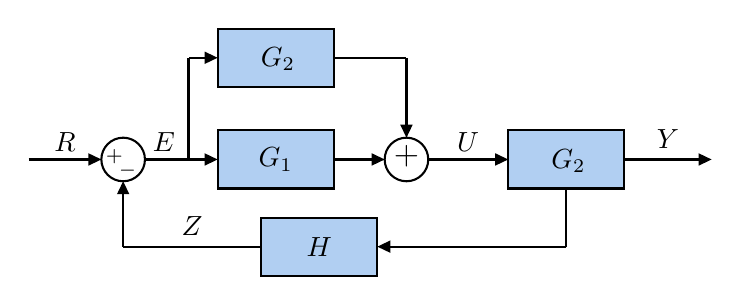
\begin{tikzpicture}[x=0.75pt,y=0.75pt,yscale=-0.7,xscale=0.7]
%uncomment if require: \path (0,300); %set diagram left start at 0, and has height of 300

%Flowchart: Process [id:dp8909683670047014] 
\draw  [fill={rgb, 255:red, 74; green, 144; blue, 226 }  ,fill opacity=0.43 ] (170,100) -- (250,100) -- (250,140) -- (170,140) -- cycle ;
%Flowchart: Process [id:dp4266368053457714] 
\draw  [fill={rgb, 255:red, 74; green, 144; blue, 226 }  ,fill opacity=0.43 ] (370,100) -- (450,100) -- (450,140) -- (370,140) -- cycle ;
%Straight Lines [id:da16159553290901518] 
\draw    (315,120) -- (367,120) ;
\draw [shift={(370,120)}, rotate = 180] [fill={rgb, 255:red, 0; green, 0; blue, 0 }  ][line width=0.08]  [draw opacity=0] (8.93,-4.29) -- (0,0) -- (8.93,4.29) -- cycle    ;
%Straight Lines [id:da64488632586266] 
\draw    (450,120) -- (507,120) ;
\draw [shift={(510,120)}, rotate = 180] [fill={rgb, 255:red, 0; green, 0; blue, 0 }  ][line width=0.08]  [draw opacity=0] (8.93,-4.29) -- (0,0) -- (8.93,4.29) -- cycle    ;
%Straight Lines [id:da3343764694846897] 
\draw    (40,120) -- (87,120) ;
\draw [shift={(90,120)}, rotate = 180] [fill={rgb, 255:red, 0; green, 0; blue, 0 }  ][line width=0.08]  [draw opacity=0] (8.93,-4.29) -- (0,0) -- (8.93,4.29) -- cycle    ;
%Flowchart: Process [id:dp29269250331680907] 
\draw  [fill={rgb, 255:red, 74; green, 144; blue, 226 }  ,fill opacity=0.43 ] (200,160) -- (280,160) -- (280,200) -- (200,200) -- cycle ;
%Straight Lines [id:da331373060110178] 
\draw    (410,140) -- (410,180) ;
%Straight Lines [id:da9734185636246361] 
\draw    (410,180) -- (283,180) ;
\draw [shift={(280,180)}, rotate = 360] [fill={rgb, 255:red, 0; green, 0; blue, 0 }  ][line width=0.08]  [draw opacity=0] (8.93,-4.29) -- (0,0) -- (8.93,4.29) -- cycle    ;
%Shape: Circle [id:dp36734656801806465] 
\draw   (90,120) .. controls (90,111.72) and (96.72,105) .. (105,105) .. controls (113.28,105) and (120,111.72) .. (120,120) .. controls (120,128.28) and (113.28,135) .. (105,135) .. controls (96.72,135) and (90,128.28) .. (90,120) -- cycle ;
%Straight Lines [id:da15484541389436335] 
\draw    (105,180) -- (105,138) ;
\draw [shift={(105,135)}, rotate = 90] [fill={rgb, 255:red, 0; green, 0; blue, 0 }  ][line width=0.08]  [draw opacity=0] (8.93,-4.29) -- (0,0) -- (8.93,4.29) -- cycle    ;
%Straight Lines [id:da11347169426560078] 
\draw    (105,180) -- (200,180) ;
%Straight Lines [id:da23824158699910636] 
\draw    (120,120) -- (167,120) ;
\draw [shift={(170,120)}, rotate = 180] [fill={rgb, 255:red, 0; green, 0; blue, 0 }  ][line width=0.08]  [draw opacity=0] (8.93,-4.29) -- (0,0) -- (8.93,4.29) -- cycle    ;
%Flowchart: Process [id:dp052444900131132566] 
\draw  [fill={rgb, 255:red, 74; green, 144; blue, 226 }  ,fill opacity=0.43 ] (170,30) -- (250,30) -- (250,70) -- (170,70) -- cycle ;
%Shape: Circle [id:dp517269529669557] 
\draw   (285,120) .. controls (285,111.72) and (291.72,105) .. (300,105) .. controls (308.28,105) and (315,111.72) .. (315,120) .. controls (315,128.28) and (308.28,135) .. (300,135) .. controls (291.72,135) and (285,128.28) .. (285,120) -- cycle ;
%Straight Lines [id:da7564533178722307] 
\draw    (150,50) -- (150,120) ;
%Straight Lines [id:da4702571770750641] 
\draw    (167,50) -- (150,50) ;
\draw [shift={(170,50)}, rotate = 180] [fill={rgb, 255:red, 0; green, 0; blue, 0 }  ][line width=0.08]  [draw opacity=0] (8.93,-4.29) -- (0,0) -- (8.93,4.29) -- cycle    ;
%Straight Lines [id:da1599953521981431] 
\draw    (250,50) -- (300,50) ;
%Straight Lines [id:da7804122351654383] 
\draw    (300,50) -- (300,102) ;
\draw [shift={(300,105)}, rotate = 270] [fill={rgb, 255:red, 0; green, 0; blue, 0 }  ][line width=0.08]  [draw opacity=0] (8.93,-4.29) -- (0,0) -- (8.93,4.29) -- cycle    ;
%Straight Lines [id:da6283216528425289] 
\draw    (250,120) -- (282,120) ;
\draw [shift={(285,120)}, rotate = 180] [fill={rgb, 255:red, 0; green, 0; blue, 0 }  ][line width=0.08]  [draw opacity=0] (8.93,-4.29) -- (0,0) -- (8.93,4.29) -- cycle    ;

% Text Node
\draw (65,116.6) node [anchor=south] [inner sep=0.75pt]    {$R$};
% Text Node
\draw (342.5,116.6) node [anchor=south] [inner sep=0.75pt]    {$U$};
% Text Node
\draw (480,114.6) node [anchor=south] [inner sep=0.75pt]    {$Y$};
% Text Node
\draw (91,118) node [anchor=west] [inner sep=0.75pt]  [font=\scriptsize]  {$+$};
% Text Node
\draw (100,127.5) node [anchor=west] [inner sep=0.75pt]  [font=\scriptsize]  {$-$};
% Text Node
\draw (210,120) node    {$G_{1}$};
% Text Node
\draw (411.5,121) node    {$G_{2}$};
% Text Node
\draw (240,180) node    {$H$};
% Text Node
\draw (133,116.6) node [anchor=south] [inner sep=0.75pt]    {$E$};
% Text Node
\draw (152.5,174.6) node [anchor=south] [inner sep=0.75pt]    {$Z$};
% Text Node
\draw (211.5,51) node    {$G_{2}$};
% Text Node
\draw (300,118) node  [font=\large]  {$+$};


\end{tikzpicture}
    
    \caption{System Block Diagram}
    \label{fig:block diagram example}
\end{figure}
First, we may combine the two blocks that are in parallel with each other. Using the algebraic approach from before, we may understand how this impacts $U$:
\begin{gather}
    U=G_2E+G_1E
\end{gather}
We may distribute the $E$ term through, which gives us that $U=(G_1+G_2)E$. This is a common fact that we can use with block diagrams -- parallel blocks being summed together can be represented as a single block of their sum.

This gives us the following simplification of the problem:
\begin{figure}[H]
    \centering


\tikzset{every picture/.style={line width=0.75pt}} %set default line width to 0.75pt        

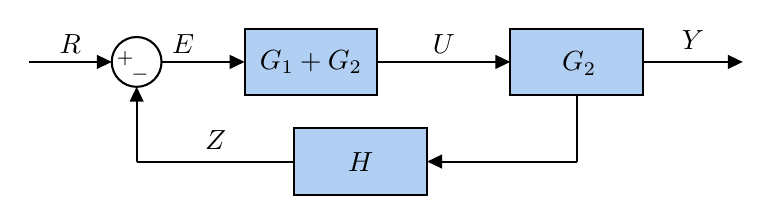
\begin{tikzpicture}[x=0.75pt,y=0.75pt,yscale=-0.8,xscale=0.8]
%uncomment if require: \path (0,300); %set diagram left start at 0, and has height of 300

%Flowchart: Process [id:dp4893171276840844] 
\draw  [fill={rgb, 255:red, 74; green, 144; blue, 226 }  ,fill opacity=0.43 ] (170,100) -- (250,100) -- (250,140) -- (170,140) -- cycle ;
%Flowchart: Process [id:dp8827980125229827] 
\draw  [fill={rgb, 255:red, 74; green, 144; blue, 226 }  ,fill opacity=0.43 ] (330,100) -- (410,100) -- (410,140) -- (330,140) -- cycle ;
%Straight Lines [id:da818348883796973] 
\draw    (250,120) -- (327,120) ;
\draw [shift={(330,120)}, rotate = 180] [fill={rgb, 255:red, 0; green, 0; blue, 0 }  ][line width=0.08]  [draw opacity=0] (8.93,-4.29) -- (0,0) -- (8.93,4.29) -- cycle    ;
%Straight Lines [id:da40590860555606645] 
\draw    (410,120) -- (467,120) ;
\draw [shift={(470,120)}, rotate = 180] [fill={rgb, 255:red, 0; green, 0; blue, 0 }  ][line width=0.08]  [draw opacity=0] (8.93,-4.29) -- (0,0) -- (8.93,4.29) -- cycle    ;
%Straight Lines [id:da5810196713768654] 
\draw    (40,120) -- (87,120) ;
\draw [shift={(90,120)}, rotate = 180] [fill={rgb, 255:red, 0; green, 0; blue, 0 }  ][line width=0.08]  [draw opacity=0] (8.93,-4.29) -- (0,0) -- (8.93,4.29) -- cycle    ;
%Flowchart: Process [id:dp8598052032893677] 
\draw  [fill={rgb, 255:red, 74; green, 144; blue, 226 }  ,fill opacity=0.43 ] (200,160) -- (280,160) -- (280,200) -- (200,200) -- cycle ;
%Straight Lines [id:da04492583655413984] 
\draw    (370,140) -- (370,180) ;
%Straight Lines [id:da9783377799879766] 
\draw    (370,180) -- (283,180) ;
\draw [shift={(280,180)}, rotate = 360] [fill={rgb, 255:red, 0; green, 0; blue, 0 }  ][line width=0.08]  [draw opacity=0] (8.93,-4.29) -- (0,0) -- (8.93,4.29) -- cycle    ;
%Shape: Circle [id:dp6771684035779256] 
\draw   (90,120) .. controls (90,111.72) and (96.72,105) .. (105,105) .. controls (113.28,105) and (120,111.72) .. (120,120) .. controls (120,128.28) and (113.28,135) .. (105,135) .. controls (96.72,135) and (90,128.28) .. (90,120) -- cycle ;
%Straight Lines [id:da3269417454883905] 
\draw    (105,180) -- (105,138) ;
\draw [shift={(105,135)}, rotate = 90] [fill={rgb, 255:red, 0; green, 0; blue, 0 }  ][line width=0.08]  [draw opacity=0] (8.93,-4.29) -- (0,0) -- (8.93,4.29) -- cycle    ;
%Straight Lines [id:da8878936380393615] 
\draw    (105,180) -- (200,180) ;
%Straight Lines [id:da7076867476551637] 
\draw    (120,120) -- (167,120) ;
\draw [shift={(170,120)}, rotate = 180] [fill={rgb, 255:red, 0; green, 0; blue, 0 }  ][line width=0.08]  [draw opacity=0] (8.93,-4.29) -- (0,0) -- (8.93,4.29) -- cycle    ;

% Text Node
\draw (65,116.6) node [anchor=south] [inner sep=0.75pt]    {$R$};
% Text Node
\draw (290,116.6) node [anchor=south] [inner sep=0.75pt]    {$U$};
% Text Node
\draw (440,114.6) node [anchor=south] [inner sep=0.75pt]    {$Y$};
% Text Node
\draw (91,118) node [anchor=west] [inner sep=0.75pt]  [font=\scriptsize]  {$+$};
% Text Node
\draw (100,127.5) node [anchor=west] [inner sep=0.75pt]  [font=\scriptsize]  {$-$};
% Text Node
\draw (210,120) node    {$G_{1} +G_{2}$};
% Text Node
\draw (371.5,121) node    {$G_{2}$};
% Text Node
\draw (240,180) node    {$H$};
% Text Node
\draw (133,116.6) node [anchor=south] [inner sep=0.75pt]    {$E$};
% Text Node
\draw (152.5,174.6) node [anchor=south] [inner sep=0.75pt]    {$Z$};


\end{tikzpicture}
    
    \caption{Simplified Block Diagram}
    \label{fig:placeholder}
\end{figure}
    With this simplification, we can use the property for the closed loop system which we derived in \eqautoref{eq:feedback law}. Doing so, we have:
    $$\frac{Y}{R}=\frac{G_2(G_1+G_2)}{1+G_2(G_1+G_2)H}$$
    For the transfer function $\frac{E}{R}$, we may do a similar argument as we did for the \eqautoref{eq:feedback law}. Doing so, we find that the general form of the error transfer function:
    $$\frac{E}{R}=\frac{1}{1+GH}$$
    So, we can find that the error transfer function takes the form:
        $$\frac{E}{R}=\frac{1}{1+G_2(G_1+G_2)H}$$
\end{example}
\begin{exercise}[Block Diagram Reduction Practice]
Consider the following system, in which we have an internal system with \textit{unity feedback} (that is, $H=1$). We have an outer feedback loop which encapsulates this unity feedback system, as shown in \autoref{fig:double feedback}.
\begin{figure}[H]
    \centering

\tikzset{every picture/.style={line width=0.75pt}} %set default line width to 0.75pt        

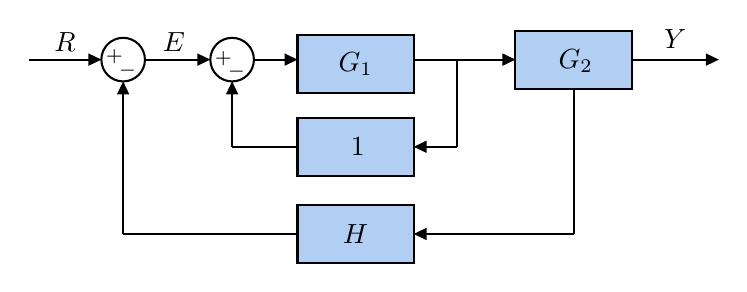
\begin{tikzpicture}[x=0.75pt,y=0.75pt,yscale=-0.7,xscale=0.7]
%uncomment if require: \path (0,300); %set diagram left start at 0, and has height of 300

%Flowchart: Process [id:dp7486957184900039] 
\draw  [fill={rgb, 255:red, 74; green, 144; blue, 226 }  ,fill opacity=0.43 ] (380,70) -- (460,70) -- (460,110) -- (380,110) -- cycle ;
%Straight Lines [id:da3299409036809947] 
\draw    (310,90) -- (377,90) ;
\draw [shift={(380,90)}, rotate = 180] [fill={rgb, 255:red, 0; green, 0; blue, 0 }  ][line width=0.08]  [draw opacity=0] (8.93,-4.29) -- (0,0) -- (8.93,4.29) -- cycle    ;
%Straight Lines [id:da5208546124786453] 
\draw    (460,90) -- (517,90) ;
\draw [shift={(520,90)}, rotate = 180] [fill={rgb, 255:red, 0; green, 0; blue, 0 }  ][line width=0.08]  [draw opacity=0] (8.93,-4.29) -- (0,0) -- (8.93,4.29) -- cycle    ;
%Straight Lines [id:da23499956313825543] 
\draw    (45,90) -- (92,90) ;
\draw [shift={(95,90)}, rotate = 180] [fill={rgb, 255:red, 0; green, 0; blue, 0 }  ][line width=0.08]  [draw opacity=0] (8.93,-4.29) -- (0,0) -- (8.93,4.29) -- cycle    ;
%Flowchart: Process [id:dp07391751731565566] 
\draw  [fill={rgb, 255:red, 74; green, 144; blue, 226 }  ,fill opacity=0.43 ] (230,190) -- (310,190) -- (310,230) -- (230,230) -- cycle ;
%Straight Lines [id:da6140340622049006] 
\draw    (420,110) -- (420,210) ;
%Straight Lines [id:da3730897255924417] 
\draw    (420,210) -- (313,210) ;
\draw [shift={(310,210)}, rotate = 360] [fill={rgb, 255:red, 0; green, 0; blue, 0 }  ][line width=0.08]  [draw opacity=0] (8.93,-4.29) -- (0,0) -- (8.93,4.29) -- cycle    ;
%Shape: Circle [id:dp9623779485713947] 
\draw   (95,90) .. controls (95,81.72) and (101.72,75) .. (110,75) .. controls (118.28,75) and (125,81.72) .. (125,90) .. controls (125,98.28) and (118.28,105) .. (110,105) .. controls (101.72,105) and (95,98.28) .. (95,90) -- cycle ;
%Straight Lines [id:da6017601045717695] 
\draw    (110,210) -- (230,210) ;
%Flowchart: Process [id:dp839390464310146] 
\draw  [fill={rgb, 255:red, 74; green, 144; blue, 226 }  ,fill opacity=0.43 ] (230,73) -- (310,73) -- (310,113) -- (230,113) -- cycle ;
%Straight Lines [id:da31038970073939487] 
\draw    (125,90) -- (167,90) ;
\draw [shift={(170,90)}, rotate = 180] [fill={rgb, 255:red, 0; green, 0; blue, 0 }  ][line width=0.08]  [draw opacity=0] (8.93,-4.29) -- (0,0) -- (8.93,4.29) -- cycle    ;
%Flowchart: Process [id:dp8576794277826157] 
\draw  [fill={rgb, 255:red, 74; green, 144; blue, 226 }  ,fill opacity=0.43 ] (230,130) -- (310,130) -- (310,170) -- (230,170) -- cycle ;
%Straight Lines [id:da07403653421600997] 
\draw    (340,90) -- (340,150) ;
%Straight Lines [id:da7112252733230411] 
\draw    (340,150) -- (313,150) ;
\draw [shift={(310,150)}, rotate = 360] [fill={rgb, 255:red, 0; green, 0; blue, 0 }  ][line width=0.08]  [draw opacity=0] (8.93,-4.29) -- (0,0) -- (8.93,4.29) -- cycle    ;
%Shape: Circle [id:dp09458014794522351] 
\draw   (170,90) .. controls (170,81.72) and (176.72,75) .. (185,75) .. controls (193.28,75) and (200,81.72) .. (200,90) .. controls (200,98.28) and (193.28,105) .. (185,105) .. controls (176.72,105) and (170,98.28) .. (170,90) -- cycle ;
%Straight Lines [id:da3818438106645917] 
\draw    (185,150) -- (185,108) ;
\draw [shift={(185,105)}, rotate = 90] [fill={rgb, 255:red, 0; green, 0; blue, 0 }  ][line width=0.08]  [draw opacity=0] (8.93,-4.29) -- (0,0) -- (8.93,4.29) -- cycle    ;
%Straight Lines [id:da24746645002259804] 
\draw    (185,150) -- (230,150) ;
%Straight Lines [id:da349151496494144] 
\draw    (200,90) -- (227,90) ;
\draw [shift={(230,90)}, rotate = 180] [fill={rgb, 255:red, 0; green, 0; blue, 0 }  ][line width=0.08]  [draw opacity=0] (8.93,-4.29) -- (0,0) -- (8.93,4.29) -- cycle    ;
%Straight Lines [id:da12166346157215358] 
\draw    (110,210) -- (110,108) ;
\draw [shift={(110,105)}, rotate = 90] [fill={rgb, 255:red, 0; green, 0; blue, 0 }  ][line width=0.08]  [draw opacity=0] (8.93,-4.29) -- (0,0) -- (8.93,4.29) -- cycle    ;

% Text Node
\draw (70,86.6) node [anchor=south] [inner sep=0.75pt]    {$R$};
% Text Node
\draw (490,84.6) node [anchor=south] [inner sep=0.75pt]    {$Y$};
% Text Node
\draw (96,88) node [anchor=west] [inner sep=0.75pt]  [font=\scriptsize]  {$+$};
% Text Node
\draw (105,97.5) node [anchor=west] [inner sep=0.75pt]  [font=\scriptsize]  {$-$};
% Text Node
\draw (421.5,91) node    {$G_{2}$};
% Text Node
\draw (270,210) node    {$H$};
% Text Node
\draw (145,86.6) node [anchor=south] [inner sep=0.75pt]    {$E$};
% Text Node
\draw (171,89) node [anchor=west] [inner sep=0.75pt]  [font=\scriptsize]  {$+$};
% Text Node
\draw (180,98.5) node [anchor=west] [inner sep=0.75pt]  [font=\scriptsize]  {$-$};
% Text Node
\draw (270,93) node    {$G_{1}$};
% Text Node
\draw (271.5,150) node    {$1$};


\end{tikzpicture}

    \caption{Two-layer feedback system}
    \label{fig:double feedback}
\end{figure}

\begin{enumerate}[label=\alph*.]
    \item Consider the unity feedback system as our plant, $P(s)$. Rewrite the block diagram with $P(s)$ in terms of $G_1(s)$ in a single block.
    \item Find the transfer function from $\frac{Y}{R}$.
    \item Think about the advantages such a system might have. Why would it be advantageous to have two feedback loops? What could some downsides be?
\end{enumerate}    
\end{exercise}

In these examples and exercises, we have covered most of the basic block diagram reduction tools that are needed. However, there are scenarios in which we encounter complex block diagrams and the reduction is more complex. In such a case, we can follow a sort of `cookbook' to find the transfer function in any case:
\begin{enumerate}
    \item Simply any parts of the system with already known relationships (feedback loop, parallel junction, multiplication in series).
    \item Label each of the connections between blocks with a variable, and write a system of equations.
    \item Solve the system of equations by making substitutions and finding an expression in terms of only the variables of interest (when finding $\frac{Y}{R}$, we would like an expression in terms of only $Y$, $R$, and any $G$'s or $H$'s which are neccesary). All of the variables of the connections should be eliminated.
    \item Use the solved system to express the transfer function of interest.
\end{enumerate}

With that, we have all the principle knowledge to create a transfer function from a block diagram, or to construct one from a differential equation using the \gls{laplace transform}. Our objective now is to understand how we may use these transfer functions to understand aspects of our system. A natural starting place is using the transfer function to understand stability.

\section{Stability}
One key criteria in control theory is studying the stability of a system. Simply stated, the stability of a system describes the tendency of a system to either return to an equilibrium position or to deviate from equilibrium. Systems that are stable tend to return to equilibrium, and those that are unstable tend to grow in magnitude and depart from their initial configuration. A simple representation of stability is the example of a ball in a valley or on a hill (\autoref{fig:stability}):
\begin{figure}[ht]
    \centering

\tikzset{every picture/.style={line width=0.75pt}} %set default line width to 0.75pt        

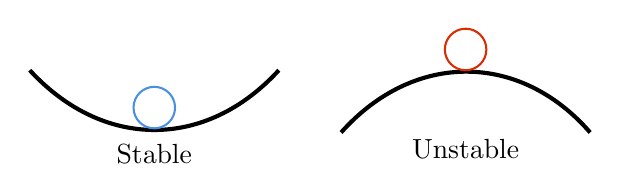
\begin{tikzpicture}[x=0.75pt,y=0.75pt,yscale=-1,xscale=1]
%uncomment if require: \path (0,300); %set diagram left start at 0, and has height of 300

%Curve Lines [id:da8058765151147705] 
\draw [line width=1.5]    (130,130) .. controls (165.34,168.38) and (214.89,168.38) .. (250,130) ;
%Curve Lines [id:da6881071931117869] 
\draw [line width=1.5]    (280,160) .. controls (315.34,120.48) and (366.44,121.34) .. (400,160) ;
%Shape: Circle [id:dp8279307439533751] 
\draw  [color={rgb, 255:red, 74; green, 144; blue, 226 }  ,draw opacity=1 ] (180,148) .. controls (180,142.48) and (184.48,138) .. (190,138) .. controls (195.52,138) and (200,142.48) .. (200,148) .. controls (200,153.52) and (195.52,158) .. (190,158) .. controls (184.48,158) and (180,153.52) .. (180,148) -- cycle ;
%Shape: Circle [id:dp17725528305328864] 
\draw  [color={rgb, 255:red, 218; green, 44; blue, 0 }  ,draw opacity=1 ] (330,120) .. controls (330,114.48) and (334.48,110) .. (340,110) .. controls (345.52,110) and (350,114.48) .. (350,120) .. controls (350,125.52) and (345.52,130) .. (340,130) .. controls (334.48,130) and (330,125.52) .. (330,120) -- cycle ;

% Text Node
\draw (190,164) node [anchor=north] [inner sep=0.75pt]   [align=left] {Stable};
% Text Node
\draw (340,162) node [anchor=north] [inner sep=0.75pt]   [align=left] {Unstable};

\end{tikzpicture}
    
    \caption{Stability}
    \label{fig:stability}
\end{figure}

In both states, the ball is at an equilibrium where the slope of the ground is zero. However, if the stable system is perturbed, the ball naturally goes back to center. In the unstable system, the ball will continue to roll down the hill and gain energy. In this example, the notion of stability is quite simple. However, it becomes useful in our study of control theory to find mathematical means of representing stability.

Before we start, we should remind ourselves why we want to study stability. One of the main objectives of control theory is to build a controller, typically denoted $u$, which can either enhance the stability of a system or turn an unstable system into one that is stable. As such, learning how to make a system stable -- and how stable it is -- is important to study.

In control theory, there are several notions of stability. As you become more advanced in your studies, different notions of stability will become to important in different contexts. However, we should establish a baseline notion of stability for linear systems. Our simplest definition of stability is this -- as $t\rightarrow\infty$, our state should converge to a final value. This is \textit{complete stability}. Something like a sine wave does not exhibit this characteristic, because it will forever oscillate between $1$ and $-1$. We call that behavior \textit{marginal stability}.

Our description with transfer functions is especially useful for understanding the stability of a system. This is because the transfer function of a system contains the information about the stability in the poles of the transfer function!

We briefly introduced the concept of poles when talking about the sine wave. The poles of a function are the values where the denominator of our transfer function is $0$. We typically denote the transfer function as a numerator and denominator polynomial in $s$:\endnote{Not all transfer functions can be written this way, but we will explore that more later in this chapter.}
$$G(s)=\frac{N(s)}{D(s)}=\frac{(s-z_1)(s-z_2)\cdots(s-z_n)}{(s-p_1)(s-p_2)\cdots(s-p_n)}$$
So, the poles of this transfer function are given by the solutions of $(s-p_1)(s-p_2)\cdots(s-p_n)=0$ and the zeros are given by $(s-z_1)(s-z_2)\cdots(s-z_n)=0$.

All of the information about the stability is given by the location of the poles in the system. When we are close to one of the pole locations, $p_n$, our denominator becomes closer and closer to $0$. Eventually, we reach the pole location exactly, and the function explodes off to $\infty$. Let's remember our example of a mass spring damper, where we had seen that:
$$G(s)=\frac{1}{ms^2+cs+k}$$
This denominator, we had seen, was a precise indication of the dynamics of the mass-spring-damper system. We have supposed that when $ms^2+cs+k=0$, we have found the exact criteria to understand the stability of the system. We have seen the pole-zero plots before, where we can represent the locations of the poles or zeros of a function in the complex plane $\mathbb{C}$. Now, we can explore some more general cases to understand stability. Consider the pole-zero plot shown in \autoref{fig:pole zero}.
\begin{figure}[ht]
    \centering


\tikzset{every picture/.style={line width=0.75pt}} %set default line width to 0.75pt        

\begin{tikzpicture}[x=0.75pt,y=0.75pt,yscale=-1,xscale=1]
%uncomment if require: \path (0,300); %set diagram left start at 0, and has height of 300

%Straight Lines [id:da6143378059913305] 
\draw    (330,60) -- (330,220) ;
%Straight Lines [id:da32627873590921797] 
\draw    (410,140) -- (250,140) ;
%Straight Lines [id:da37253286393851626] 
\draw [color={rgb, 255:red, 218; green, 44; blue, 0 }  ,draw opacity=1 ]   (350,100) ;
\draw [shift={(350,100)}, rotate = 45] [color={rgb, 255:red, 218; green, 44; blue, 0 }  ,draw opacity=1 ][line width=0.75]    (-5.59,0) -- (5.59,0)(0,5.59) -- (0,-5.59)   ;
%Straight Lines [id:da11664231471930675] 
\draw [color={rgb, 255:red, 218; green, 44; blue, 0 }  ,draw opacity=1 ]   (350,180) ;
\draw [shift={(350,180)}, rotate = 45] [color={rgb, 255:red, 218; green, 44; blue, 0 }  ,draw opacity=1 ][line width=0.75]    (-5.59,0) -- (5.59,0)(0,5.59) -- (0,-5.59)   ;

% Text Node
\draw (348,52.4) node [anchor=north west][inner sep=0.75pt]    {$\mathbb{C}$};
% Text Node
\draw (323,40.4) node [anchor=north west][inner sep=0.75pt]    {$\omega $};
% Text Node
\draw (414,130.4) node [anchor=north west][inner sep=0.75pt]    {$\sigma $};


\end{tikzpicture}
    
    \caption{General Pole-Zero Plot}
    \label{fig:pole zero}
\end{figure}

Here, the function has poles at $s=\sigma\pm i\omega$ in the $s$-domain. From our discussion of the \gls{laplace transform}, this means that the behavior of the system in the time domain can be represented by  $e^{st}$, which gives
$$f(t)=e^{(\sigma\pm i\omega)t}=e^{\sigma t}e^{i\omega t}$$
We have previously shown that $e^{i\omega t}$ always has a magnitude of 1 and simply represents rotation in the complex plane. As a result, the magnitude of $f(t)$ is purely dictated by the term $e^{\sigma t}$.

We know that for $t>0$, $e^{\sigma t}$ will grow unbounded for $\sigma >0$ and will converge to $0$ for $\sigma < 0$. These values for $\sigma$ then, dictate the stability of our system. In the pole-zero diagram, we can represent this diagrammatically as shown in \autoref{fig:pole zero stability}.
\begin{figure}
    \centering
% Pattern Info
 
\tikzset{
pattern size/.store in=\mcSize, 
pattern size = 5pt,
pattern thickness/.store in=\mcThickness, 
pattern thickness = 0.3pt,
pattern radius/.store in=\mcRadius, 
pattern radius = 1pt}
\makeatletter
\pgfutil@ifundefined{pgf@pattern@name@_9yu0p9uwl}{
\pgfdeclarepatternformonly[\mcThickness,\mcSize]{_9yu0p9uwl}
{\pgfqpoint{0pt}{0pt}}
{\pgfpoint{\mcSize+\mcThickness}{\mcSize+\mcThickness}}
{\pgfpoint{\mcSize}{\mcSize}}
{
\pgfsetcolor{\tikz@pattern@color}
\pgfsetlinewidth{\mcThickness}
\pgfpathmoveto{\pgfqpoint{0pt}{0pt}}
\pgfpathlineto{\pgfpoint{\mcSize+\mcThickness}{\mcSize+\mcThickness}}
\pgfusepath{stroke}
}}
\makeatother

% Pattern Info
 
\tikzset{
pattern size/.store in=\mcSize, 
pattern size = 5pt,
pattern thickness/.store in=\mcThickness, 
pattern thickness = 0.3pt,
pattern radius/.store in=\mcRadius, 
pattern radius = 1pt}
\makeatletter
\pgfutil@ifundefined{pgf@pattern@name@_pm1rnvitx}{
\pgfdeclarepatternformonly[\mcThickness,\mcSize]{_pm1rnvitx}
{\pgfqpoint{0pt}{-\mcThickness}}
{\pgfpoint{\mcSize}{\mcSize}}
{\pgfpoint{\mcSize}{\mcSize}}
{
\pgfsetcolor{\tikz@pattern@color}
\pgfsetlinewidth{\mcThickness}
\pgfpathmoveto{\pgfqpoint{0pt}{\mcSize}}
\pgfpathlineto{\pgfpoint{\mcSize+\mcThickness}{-\mcThickness}}
\pgfusepath{stroke}
}}
\makeatother
\tikzset{every picture/.style={line width=0.75pt}} %set default line width to 0.75pt        

\begin{tikzpicture}[x=0.75pt,y=0.75pt,yscale=-1,xscale=1]
%uncomment if require: \path (0,300); %set diagram left start at 0, and has height of 300

%Shape: Rectangle [id:dp6154325357400674] 
\draw  [draw opacity=0][pattern=_9yu0p9uwl,pattern size=6pt,pattern thickness=0.75pt,pattern radius=0pt, pattern color={rgb, 255:red, 74; green, 144; blue, 226}] (261,90) -- (340,90) -- (340,250) -- (261,250) -- cycle ;
%Shape: Rectangle [id:dp04797856148304802] 
\draw  [draw opacity=0][pattern=_pm1rnvitx,pattern size=6pt,pattern thickness=0.75pt,pattern radius=0pt, pattern color={rgb, 255:red, 218; green, 44; blue, 0}] (340,90) -- (419,90) -- (419,250) -- (340,250) -- cycle ;
%Straight Lines [id:da511814457639373] 
\draw    (340,90) -- (340,250) ;
%Straight Lines [id:da5970664610164672] 
\draw    (420,170) -- (260,170) ;

% Text Node
\draw (333,70.4) node [anchor=north west][inner sep=0.75pt]    {$\omega $};
% Text Node
\draw (424,160.4) node [anchor=north west][inner sep=0.75pt]    {$\sigma $};
% Text Node
\draw (278,72.4) node [anchor=north west][inner sep=0.75pt]  [color={rgb, 255:red, 74; green, 144; blue, 226 }  ,opacity=1 ]  {$stable$};
% Text Node
\draw (353,72.4) node [anchor=north west][inner sep=0.75pt]  [color={rgb, 255:red, 218; green, 44; blue, 0 }  ,opacity=1 ]  {$unstable$};


\end{tikzpicture}
    \caption{Stability Criteria on Pole Zero Plot}
    \label{fig:pole zero stability}
\end{figure}
Our resulting stability criteria is this: \textbf{If all poles of the transfer function are in the left half of the complex plane, then the transfer function is stable.}

\newpage
\begin{exercise}[Mass Spring Damper Poles]
Consider again the mass spring damper system. Where do the poles of this function lie? For positive values of the coefficients $m,k$ and $c$, what can you say about the stability of the system?
\end{exercise}

\subsection{Routh Stability Criterion}
    
One important rule in the determination of the stability of a system is the Routh stability criterion. It is often the case that our denominator polynomial is not in a nice form - like $(s-p_1)(s-p_2)(s-p_3)$. Instead, it is much more often that we found our denominator in a form like $s^4-3s^2+2s+6$. This presents us with a problem. For cases where the order of the polynomial is small, like $s^2$ or $s^3$, we may easily compute the exact location of the poles using the quadratic or cubic formulas. However, once we reach a 5th order polynomial or higher, an analytical solution for the roots of a polynomial no longer exists in general.\endnote{Interesting, this may be proved using discrete groups and their permutations, which is the subject of \textit{Galois Theory}.} 

Luckily, our desires are not so grand. We don't need to know the exact location of the poles, but only if the real part of the poles are positive or negative. This is all we require to determine if the system is stable or not, after all! What we would like to do is develop a simple test which can tell us if such a polynomial is stable or not. Of course, modern computers can numerically approximate the locations of poles, but often we still want to know what condition is required to make the system stable.

It turns out that we can develop such a test, which we call the Routh-Hurwitz stability criterion. The proof of this criterion is beyond the scope of this current text. Here, it will suffice to show how we may use it.

First, we construct a table with the coefficients of our polynomial, $P(s)$, and write $s^n,s^{n-1},\cdots ,s^0$  down the first column. The coefficients of the polynomial then go across the first two rows, top to bottom, and then left to right. Supposing our polynomial is $s^3+2s^2+4s+6$, this pattern would give us:

$$
\begin{array}{lcc}
     s^3& 1 &4\\
     s^2& 2&6\\
     s^1& \\
     s^0
\end{array}
$$
We assign the rest of the rows with $[a_1\cdots a_n]$, $[b_1\cdots b_n]$, and so on:
$$
\begin{array}{lcc}
     s^3& 1 &4\\
     s^2& 2&6\\
     s^1&a_1&a_2 \\
     s^0&b_1
\end{array}
$$
For $a_1$, we compute the $-\det$ of the four elements, shown in red:
$$
\begin{array}{lcc}
     s^3& \color{red}1 &\color{red}4\\
     s^2& \color{red}2&\color{red}6\\
     s^1&a_1&a_2 \\
     s^0&b_1
\end{array}
$$
and divide by the element in red which occupies the lower left corner (value of 2). Thus, we have:
$$a_1=\frac{-\begin{vmatrix}1&4\\2&6
\end{vmatrix}}{2}=\frac{4\cdot2-1\cdot6}{2}=1$$
For $a_2$, we follow a similar argument, but the second column of the determinant is instead the column above $a_2$ and to the right (shown in blue):
$$
\begin{array}{lccc}
     s^3& \color{red}1 &4&\color{blue}0\\
     s^2& \color{red}2&6&\color{blue}0\\
     s^1&1&a_2 \\
     s^0&b_1
\end{array}
$$
The elements in red remain the same, such that $a_2$ is:
$$a_2=\frac{-\begin{vmatrix}1&0\\2&0
\end{vmatrix}}{2}=0$$
We follow the same argument to construct $b_1$, with the appropriate elements again highlighted in red:
$$
\begin{array}{lcc}
     s^3& 1 &4\\
     s^2& \color{red}2&\color{red}6\\
     s^1&\color{red}1&\color{red}0 \\
     s^0&b_1
\end{array}
$$
From which we have:
$$a_1=\frac{-\begin{vmatrix}2&6\\1&0
\end{vmatrix}}{1}=6\cdot1=6$$
We continue until we have filled out the table down to the $s^0$ term. This gives us the full Routh table:
$$
\begin{array}{lcc}
     s^3& 1 &4\\
     s^2& 2&6\\
     s^1&1&0 \\
     s^0&6
\end{array}
$$
After completing the table, we should look in the left-hand column of values (here, $[1,2,1,6]^\top$). If all these values are positive, then the polynomial is stable. We may verify this by computing the roots of this polynomial in MATLAB using "roots([1 2 4 6])". This returns our three roots:

"[-0.1443 + 1.8669i, -0.1443 - 1.8669i, -1.7113]" 

As we can see, the system has negative roots and is indeed stable.

\begin{example}[Routh Criterion of Quintic Polynomial]
    It is a common mathematical fact that the roots of a quintic polynomial do not have a closed form solution using radicals. However, we can still apply Routh's criteria on such a polynomial. Let's consider the polynomial
    $$s^5+3s^4+2s^3+4s^2+1=0$$
    We may begin the construction of the Routh table in the typical way, placing each coefficient of the polynomial in the first two rows. Notice that since no term exists in $s$, this value is $0$.
    $$
    \begin{array}{lccc}
         s^5&1&2&0  \\
         s^4&3&4&1\\
         s^3&a_1&a_2\\
         s^2&b_1&b_2\\
         s^1&c_1\\
         s^0&d_1
    \end{array}
    $$
    The values which must be calculated are also shown. To compute $a_1$, we follow the formula:
    $$a_1=\frac{-\begin{vmatrix}
        1&0\\3&1
    \end{vmatrix}}{3}=\frac{6-4}{3}=\frac{2}{3}$$
    We compute $a_2$ in a similar way:
        $$a_2=\frac{-\begin{vmatrix}
        1&0\\3&1
    \end{vmatrix}}{3}=\frac{0-1}{3}=-\frac{1}{3}$$
    For $b$, we can compute using the values we have attained for $a_1$ and $a_2$. This gives:
        $$b_1=\frac{-\begin{vmatrix}
        3&4\\\frac{2}{3}&-\frac{1}{3}
    \end{vmatrix}}{\frac{2}{3}}=\frac{\frac{8}{3}+1}{\frac{2}{3}}=\frac{11}{2}$$
$$b_2=\frac{-\begin{vmatrix}
        3&1\\\frac{2}{3}&0
    \end{vmatrix}}{\frac{2}{3}}=\frac{\frac{2}{3}}{\frac{2}{3}}=1$$
    We continue this same process, taking the two rows aboce the current value of interest. For $c_1$:
     $$c_1=\frac{-\begin{vmatrix}
        \frac{2}{3}&-\frac{1}{3}\\\frac{11}{2}&1
    \end{vmatrix}}{\frac{11}{2}}=\frac{-\frac{11}{6}-\frac{2}{3}}{\frac{11}{2}}=-\frac{5}{11}$$
    Finally, $d_1$:
         $$d_1=\frac{-\begin{vmatrix}
        \frac{11}{2}&1\\\frac{5}{11}&0
    \end{vmatrix}}{\frac{5}{11}}=\frac{\frac{5}{11}}{\frac{5}{11}}=1$$
Together, the completed Routh table is:
    $$
    \begin{array}{lccc}
         s^5&1&2&0  \\
         s^4&3&4&1\\
         s^3&\frac{2}{3}&-\frac{1}{3}\\
         s^2&\frac{11}{2}&1\\
         s^1&-\frac{5}{11}\\
         s^0&1
    \end{array}
    $$
We see that the entry in the $s^1$ row is negative, so this polynomial must have a root with positive real part. How many such roots? If we count the number of sign changes in the first column, we can determine the number of positive roots.
    $$
    \begin{array}{lc}
         s^5&+ \\
         s^4&+\\
         s^3&+\\
         s^2&+\\
         s^1&-\\
         s^0&+
    \end{array}
    $$
    We can see that there are \textit{two} sign flips, from $+\rightarrow-$ going from $s^2$ to $s^1$, and another when we go from $s^1$ to $s^0$ ($-\rightarrow+$). This tells us that this polynomial has two roots with positive real part. Using a numerical solver, we can indeed confirm this.
\end{example}
\begin{exercise}[Routh Criterion Consequences]
Use the Routh Hurwitz Criterion to show that each element of a polynomial $P(s)$ must have the same sign in order for the criteria to hold. Start with the case of $as^3+bs^2+cs+d$, showing that $a,b,c,d>0$ (or all are negative, which is equivalent). Generalize this to a polynomial of any degree.
\end{exercise}
\begin{exercise}[Routh Stability Criterion with a variable]
    Consider a polynomial $s^3+3s^2+ks+3$. Find the value(s) of $k$ such that the system is stable.
\end{exercise}

As we saw in the last exercise, the Routh stability criterion has the interesxting property that it allows us to determine whether a system will be stable under certain conditions. \textbf{If we have direct control over that value, $k$, we may alter the stability of the system!} Choosing appropriate values of $k$ is one good way that we may systematically construct a controller. We'll keep that idea in mind -- that we can choose different values of $k$ to change the stability -- when we go to start developing controllers.

\subsection{Special Cases of Routh Stability Criterion}
Sometimes we run into some problems when following the procedure for the Routh stability criterion which is detailed above.

\subsubsection{Special Case 1}
One such special case is when we have a number in the first column which is equal to $0$. Consider the following case:
    $$
    \begin{array}{lccc}
         s^5&1&2&4  \\
         s^4&3&6&9\\
         s^3&a_1&a_2\\
         s^2&&\\
         s^1&\\
         s^0&
    \end{array}
    $$
    Computation of $a_1$ reveals that:
        $$a_1=\frac{-\begin{vmatrix}
        1&2\\3&6
    \end{vmatrix}}{3}=\frac{6-6}{3}=0$$
    However, $a_2$ is a non-zero term:
            $$a_2=\frac{-\begin{vmatrix}
        1&4\\3&9
    \end{vmatrix}}{3}=\frac{12-9}{3}=1$$
    In such a case, we replace the $a_1$ term by a variable $\varepsilon$. We choose this variable with the intention that $\varepsilon$ is a small number, close to 0, which will give us information about the sign changes (which we would not have if we proceeded forward using $0$). Completing the table from this point as we ordinarily would:
        $$
    \begin{array}{lccc}
         s^5&1&2&4  \\
         s^4&3&6&9\\
         s^3&\varepsilon&1\\
         s^2&6-\frac{3}{\varepsilon}&9\\
         s^1&1-\frac{3\varepsilon^2}{2\varepsilon-1}\\
         s^0&9
    \end{array}
    $$
    Now, we consider $\varepsilon$ to take on a small value, $|\varepsilon|\ll1$. We can either take $\varepsilon$ to be negative or positive, either gives the same final result. Here, let's choose $\varepsilon$ to be a small positive value. We may evaluate the statements in the first row, which gives:
    \begin{gather}
        \varepsilon\rightarrow +\\
        6-\frac{3}{\varepsilon}\rightarrow -\\
        1-\frac{3\varepsilon^2}{2\varepsilon-1}\rightarrow+
    \end{gather}
We see that $6-\frac{3}{\varepsilon}$ is the only statement which is negative, as $-\frac{1}{\varepsilon}$ tends towards $-\infty$. We can see that a sign change must have occured, and the system is not stable.

\subsubsection{Special Case 2}
Our second special case occurs when an entire row of our polynomial is zero. This will occur if two rows are exactly identical, leading the determinant to be zero for an entire row. An example is:
$$
    \begin{array}{lccc}
         s^5&1&3&5  \\
         s^4&1&3&5\\
         s^3&a_1&a_2\\
         s^2&&\\
         s^1&\\
         s^0&
    \end{array}
    $$
    Computation of $a_1$ and $a_2$ shows that this entire row is $0$. We cannot employ the same trick as before, as our determinants will be $0$ for the rest of the sequence. In this special case, we take the row above, here $s^4$, and write the polynomial corresponding to this: $$P=s^4+3s^2+5$$
    We find the derivative of this polynomial with respect to $s$, which gives the $s^3$ row:
    $$P'=4s^3+6s$$
    We use these coefficients in the Routh table, and proceed as normal:
    $$
    \begin{array}{lccc}
         s^5&1&3&5  \\
         s^4&1&3&5\\
         s^3&4&6\\
         s^2&\frac{3}{2}&5\\
         s^1&-\frac{22}{3}\\
         s^0&5
    \end{array}
    $$
In the case where an entire row is zeros, there are no poles in the right half plane, but purely imaginary poles are guaranteed. Thus, such a system would be marginally stable.

\section{Types of Transfer Functions}
There are a few types of transfer functions that we see very often, and it is useful to learn and understand their characteristics well. The two types that we focus on are first order systems and second order systems. We don't concern ourselves with higher order systems because we may construct them by multiplying together a combination of first and second order systems.

\subsection{First Order Systems}
First order transfer functions are some of the simplest transfer functions that we can construct. A first order transfer function represents a system which contains only a first order derivative:
$$\dot{y}=ay+bu$$
In the Laplace domain:
$$sY(s)=aY(s)+bU(s)$$
$$Y(s)(s-a)=bU(s)$$

$$\frac{Y(s)}{U(s)}=G(s)=\frac{b}{s-a}$$
As we can see, such a system yields a simple transfer function. We often choose to rewrite this by dividing by $a$ and rewrite the equation with $\tau=\frac{1}{a}$:
$$G(s)=\frac{K}{s\tau+1}$$
This type of system only has two parameters. $K$ is the gain of the system, which tells us the amplification of the transfer function. The other parameter, $\tau$, is called the time constant of the system. It informs us how quickly our system responds to an input.

\subsubsection{Step Response of First Order Systems}

We can easily compute the step response of a first order system by hand or using a computer. Let's take our system to be:
$$F(s)=\frac{1}{s+1}$$
We remember that the unit step response looks like:
$$\frac{1}{s}$$
We multiply our transfer function by this to attain the total response:
$$\frac{1}{s(s+1)}$$
We may use partial fraction decomposition to solve this system:
$$\frac{A}{s}+\frac{B}{s+1}=\frac{1}{s(s+1)}$$
The solution of which is:
$$f(t)=1-e^{-t}$$
We can similarly compute the step response in code:
\begin{matlabscript}{}
sys = tf(1,[1 1]) % transfer function

[y,tOut] = step(sys);
\end{matlabscript}
\begin{pythonscript}{}
import control as ctrl

sys = ctrl.tf([1], [1, 1])  # transfer function
t, y = ctrl.step_response(sys)
\end{pythonscript}

We see that the analytical approach is identical to the computational approach, as shown in \autoref{fig:step response first order}.
\begin{figure}[H]
    \centering
    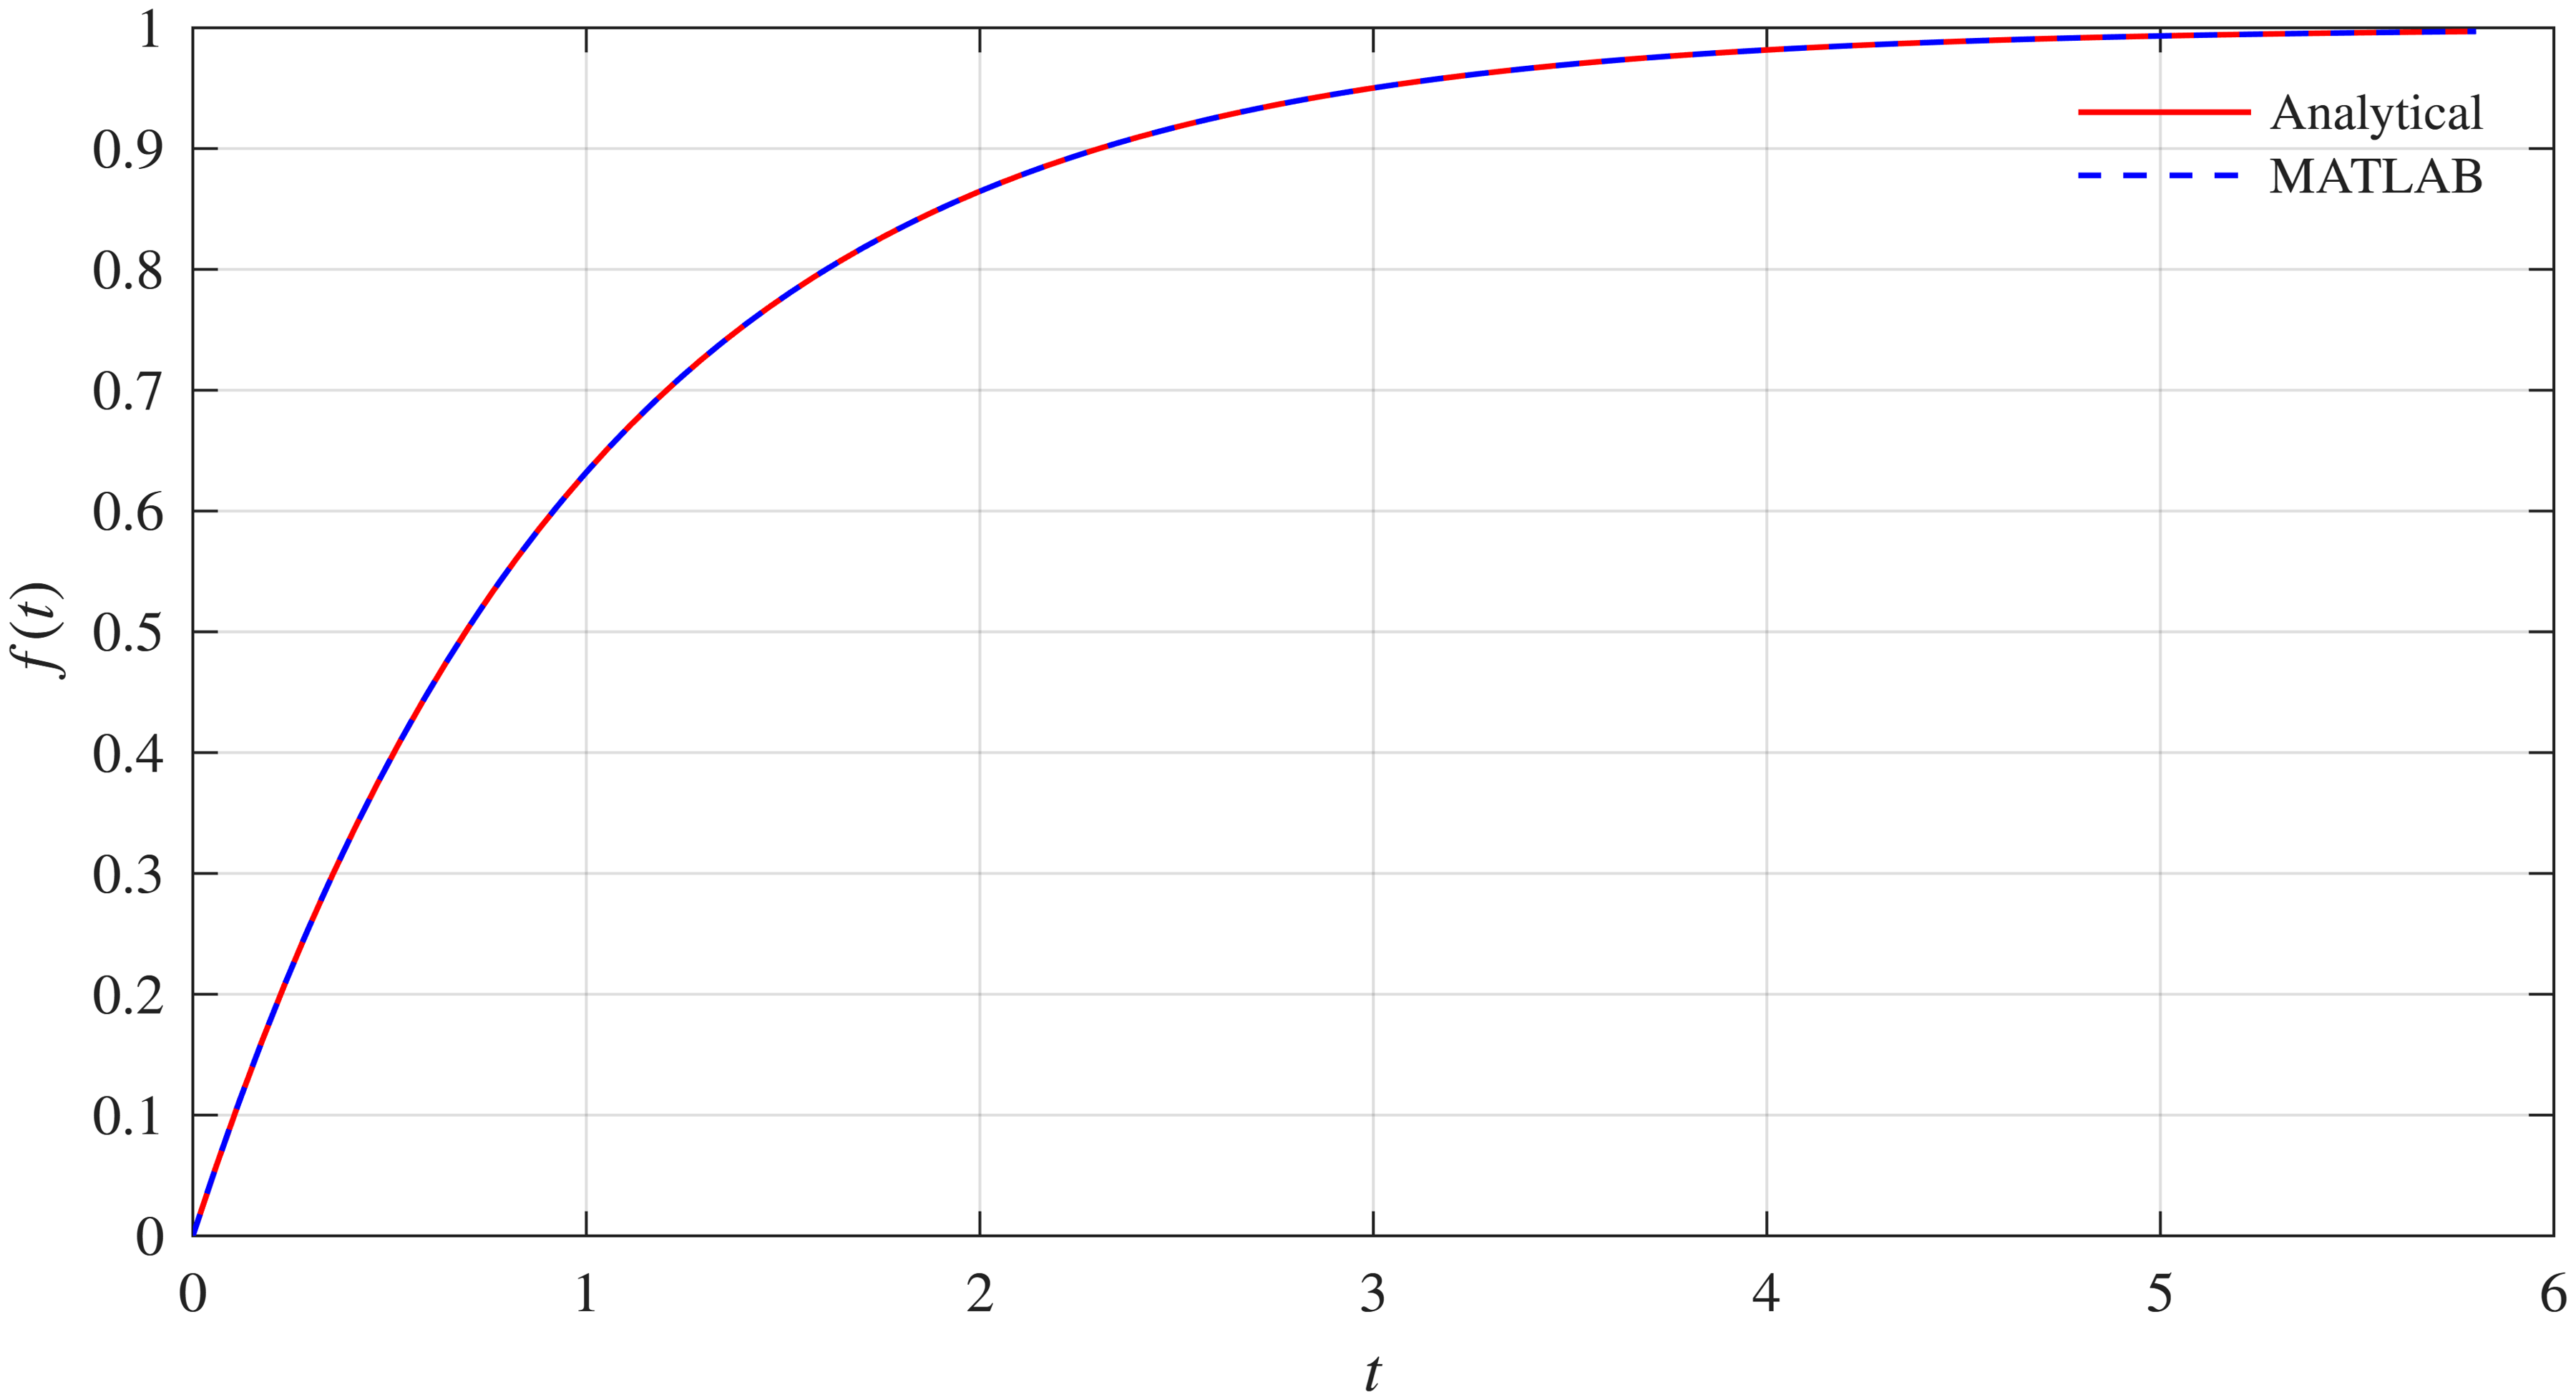
\includegraphics[width=0.75\linewidth]{StepResponse.png}
    \caption{Step Response of $\frac{1}{s+1}$}
    \label{fig:step response first order}
\end{figure}
Notice in our previous example that after $1$ second, $f(t)$ reaches $\sim63\%$ of the final value. This result is obvious when we consider that $1-e^{-t}\approx0.63$ when $t=1$. How long the function takes to reach this threshold is governed by the variable $\tau$. The numerical value of $\tau$ gives the amount of time before the system reaches this $\sim63\%$ threshold. Thus, the time constant determines how quickly a first order system can respond to an input. Of course, gain $K$ dictates the final height in the step response. In the above example, since $K=1$ and the system was subjected to a step response, the final height is $1$.

With just two parameters, we can classify any first order transfer function. We often use such transfer functions to approximate simple processes with a transient start up. Another use case of these first order systems is a \textit{low-pass filter}. We will see this behavior when we study frequency domain behaviors in \autoref{chap:frequency}.

\subsection{Second Order System}
As we have seen when doing Newtonian or Lagrangian mechanics, almost all of our physical systems are dictated by second order equations. Therefore, we can model a huge variety of physical processes by carefully studying these systems. The second order system creates oscillations, which makes it much more complicated than the first order system. The canonical form of the second order system is based on the mass spring damper system. The form of the equation is:\endnote{If you want to derive this form, you may do so in an analogous way to what we did for the first order system.}

\begin{equation}\label{2nd order tf}
G(s)=\frac{\omega_n}{s^2+\zeta\omega_ns+{\omega_n}^2}
\end{equation}

We give each of the variables in this equation a special name because they come up very frequently in engineering and physics applications. We call $\omega_n$ the natural frequency. Under the influence of no damping to the system, this is the angular frequency of the system. In a system like a mass spring damper, it is physically given as the square root of the ratio between the spring constant and the mass:
$$\omega_n=\sqrt{\frac{k}{m}}$$
The term $\zeta$ is called the \textit{damping coefficient}. The value of the damping coefficient must be positive for real systems. At a value of $\zeta=1$, we say that a system is \textit{critically damped}. This is the value at which the system will converge to the input in the least amount of time. For values of $\zeta<1$, the system is called \textit{underdamped}, and will oscillate back and forth before reaching a final value. In control theory, this means the system will have an imaginary component of the eigenvalues. When $\zeta>1$, the system is \textit{overdamped} and will show no oscillation. Here, the eigenvalues of the system will be purely real.

\subsubsection{Second Order Specifications}
The parameters of the second order transfer function are very closely related to the location of the poles of the transfer function. If we understand how to make these adjustments, we can design a second order system that behaves exactly how we want it to. We can summarize all the key features in the complex plane as shown in \autoref{fig:second order poles plot}.

\begin{figure}[ht]
    \centering




\tikzset{every picture/.style={line width=0.75pt}} %set default line width to 0.75pt        

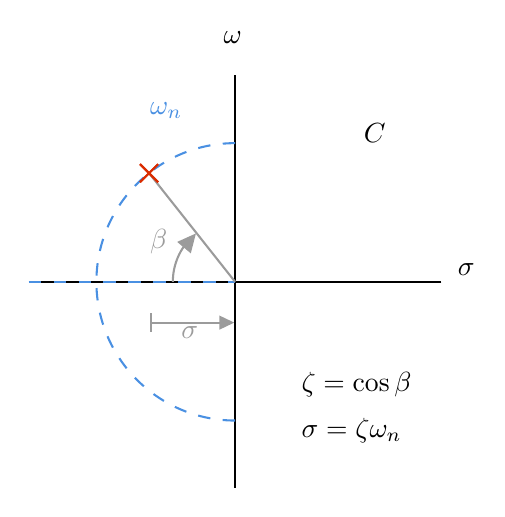
\begin{tikzpicture}[x=0.75pt,y=0.75pt,yscale=-1,xscale=1]
%uncomment if require: \path (0,300); %set diagram left start at 0, and has height of 300

%Straight Lines [id:da3243107301786887] 
\draw    (320.44,50.92) -- (320.44,249.79) ;
%Straight Lines [id:da05704068779201743] 
\draw    (419.87,150.35) -- (221,150.35) ;
%Shape: Arc [id:dp8738705238498384] 
\draw  [draw opacity=0][dash pattern={on 4.5pt off 4.5pt}] (320.44,217.18) .. controls (320.44,217.18) and (320.44,217.18) .. (320.44,217.18) .. controls (283.53,217.18) and (253.61,187.26) .. (253.61,150.35) .. controls (253.61,113.44) and (283.53,83.53) .. (320.44,83.53) -- (320.44,150.35) -- cycle ; \draw  [color={rgb, 255:red, 74; green, 144; blue, 226 }  ,draw opacity=1 ][dash pattern={on 4.5pt off 4.5pt}] (320.44,217.18) .. controls (320.44,217.18) and (320.44,217.18) .. (320.44,217.18) .. controls (283.53,217.18) and (253.61,187.26) .. (253.61,150.35) .. controls (253.61,113.44) and (283.53,83.53) .. (320.44,83.53) ;  
%Straight Lines [id:da6227885653022915] 
\draw [color={rgb, 255:red, 74; green, 144; blue, 226 }  ,draw opacity=1 ] [dash pattern={on 4.5pt off 4.5pt}]  (221,150.35) -- (320.44,150.35) ;
%Straight Lines [id:da7350291413092821] 
\draw [color={rgb, 255:red, 155; green, 155; blue, 155 }  ,draw opacity=1 ]   (320.44,150.35) -- (279,98) ;
%Shape: Arc [id:dp16286487075266098] 
\draw  [draw opacity=0] (290.44,150.35) .. controls (290.44,140.94) and (294.77,132.54) .. (301.55,127.04) -- (320.44,150.35) -- cycle ; \draw [color={rgb, 255:red, 155; green, 155; blue, 155 }  ,draw opacity=1 ]   (290.44,150.35) .. controls (290.44,141.97) and (293.87,134.4) .. (299.41,128.95) ; \draw [shift={(301.55,127.04)}, rotate = 130.03] [fill={rgb, 255:red, 155; green, 155; blue, 155 }  ,fill opacity=1 ][line width=0.08]  [draw opacity=0] (8.93,-4.29) -- (0,0) -- (8.93,4.29) -- cycle    ; 
%Straight Lines [id:da7597435504681186] 
\draw [color={rgb, 255:red, 218; green, 44; blue, 0 }  ,draw opacity=1 ]   (279,98) ;
\draw [shift={(279,98)}, rotate = 45] [color={rgb, 255:red, 218; green, 44; blue, 0 }  ,draw opacity=1 ][line width=0.75]    (-6.15,0) -- (6.15,0)(0,6.15) -- (0,-6.15)   ;
\draw [shift={(279,98)}, rotate = 45] [color={rgb, 255:red, 218; green, 44; blue, 0 }  ,draw opacity=1 ][line width=0.75]    (-6.15,0) -- (6.15,0)(0,6.15) -- (0,-6.15)   ;
%Straight Lines [id:da7948143459768348] 
\draw [color={rgb, 255:red, 155; green, 155; blue, 155 }  ,draw opacity=1 ]   (280,170) -- (317,170) ;
\draw [shift={(320,170)}, rotate = 180] [fill={rgb, 255:red, 155; green, 155; blue, 155 }  ,fill opacity=1 ][line width=0.08]  [draw opacity=0] (7.14,-3.43) -- (0,0) -- (7.14,3.43) -- cycle    ;
\draw [shift={(280,170)}, rotate = 180] [color={rgb, 255:red, 155; green, 155; blue, 155 }  ,draw opacity=1 ][line width=0.75]    (0,4.47) -- (0,-4.47)   ;

% Text Node
\draw (381,72.4) node [anchor=north west][inner sep=0.75pt]    {$\mathbb{C}$};
% Text Node
\draw (313.44,28.4) node [anchor=north west][inner sep=0.75pt]    {$\omega $};
% Text Node
\draw (426.3,140.26) node [anchor=north west][inner sep=0.75pt]    {$\sigma $};
% Text Node
\draw (278,123.4) node [anchor=north west][inner sep=0.75pt]  [color={rgb, 255:red, 155; green, 155; blue, 155 }  ,opacity=1 ]  {$\beta $};
% Text Node
\draw (278,62.4) node [anchor=north west][inner sep=0.75pt]  [color={rgb, 255:red, 74; green, 144; blue, 226 }  ,opacity=1 ]  {$\omega _{n}$};
% Text Node
\draw (351,192.4) node [anchor=north west][inner sep=0.75pt]    {$\zeta =\cos \beta $};
% Text Node
\draw (293,170.4) node [anchor=north west][inner sep=0.75pt]  [color={rgb, 255:red, 155; green, 155; blue, 155 }  ,opacity=1 ]  {$\sigma $};
% Text Node
\draw (351,214.4) node [anchor=north west][inner sep=0.75pt]    {$\sigma =\zeta \omega _{n}$};


\end{tikzpicture}

    \caption{Relation of second order system values to pole locations}
    \label{fig:second order poles plot}
\end{figure}

In the diagram, the poles may exist on any portion of the dotted blue line. The radius of the circular region of the dotted blue line is given by $\omega_n$. The distance from the imaginary axis is $\sigma=\zeta\omega_n$. The angle of the pole from the horizontal is given by the relation $\zeta=\cos\beta$. You may notice that when $\zeta=1$, the angle must be zero. The result is that the critically damped system has both poles lying exactly on the furthest possible point from the origin. Therefore, this is the system which decays the fastest. For greater values, the constraint breaks down because $\cos$ can never achieve a value greater than 1. After this point, the poles stay fixed on the real line. We can represent all possible scenarios as shown in \autoref{fig:pole zeta}:
\begin{figure}[ht]
    \centering

\tikzset{every picture/.style={line width=0.75pt}} %set default line width to 0.75pt        

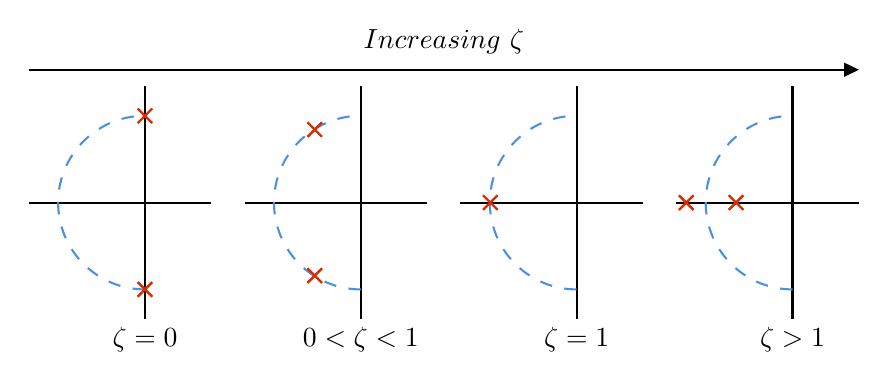
\begin{tikzpicture}[x=0.75pt,y=0.75pt,yscale=-0.8,xscale=0.8]
%uncomment if require: \path (0,300); %set diagram left start at 0, and has height of 300

%Straight Lines [id:da5282441780493525] 
\draw    (100,70) -- (100,210) ;
%Straight Lines [id:da7423345996136652] 
\draw    (140,140) -- (30,140) ;
%Shape: Arc [id:dp3799084322094477] 
\draw  [draw opacity=0][dash pattern={on 4.5pt off 4.5pt}] (100,192.28) .. controls (100,192.28) and (100,192.28) .. (100,192.28) .. controls (71.13,192.28) and (47.72,168.87) .. (47.72,140) .. controls (47.72,111.13) and (71.13,87.72) .. (100,87.72) -- (100,140) -- cycle ; \draw  [color={rgb, 255:red, 74; green, 144; blue, 226 }  ,draw opacity=1 ][dash pattern={on 4.5pt off 4.5pt}] (100,192.28) .. controls (100,192.28) and (100,192.28) .. (100,192.28) .. controls (71.13,192.28) and (47.72,168.87) .. (47.72,140) .. controls (47.72,111.13) and (71.13,87.72) .. (100,87.72) ;  
%Straight Lines [id:da7728653865582944] 
\draw    (30,60) -- (527,60) ;
\draw [shift={(530,60)}, rotate = 180] [fill={rgb, 255:red, 0; green, 0; blue, 0 }  ][line width=0.08]  [draw opacity=0] (8.93,-4.29) -- (0,0) -- (8.93,4.29) -- cycle    ;
%Straight Lines [id:da3227845193340638] 
\draw [color={rgb, 255:red, 218; green, 44; blue, 0 }  ,draw opacity=1 ]   (100,87.72) ;
\draw [shift={(100,87.72)}, rotate = 45] [color={rgb, 255:red, 218; green, 44; blue, 0 }  ,draw opacity=1 ][line width=0.75]    (-6.15,0) -- (6.15,0)(0,6.15) -- (0,-6.15)   ;
\draw [shift={(100,87.72)}, rotate = 45] [color={rgb, 255:red, 218; green, 44; blue, 0 }  ,draw opacity=1 ][line width=0.75]    (-6.15,0) -- (6.15,0)(0,6.15) -- (0,-6.15)   ;
%Straight Lines [id:da8934356003374623] 
\draw [color={rgb, 255:red, 218; green, 44; blue, 0 }  ,draw opacity=1 ]   (100,192.28) ;
\draw [shift={(100,192.28)}, rotate = 45] [color={rgb, 255:red, 218; green, 44; blue, 0 }  ,draw opacity=1 ][line width=0.75]    (-6.15,0) -- (6.15,0)(0,6.15) -- (0,-6.15)   ;
\draw [shift={(100,192.28)}, rotate = 45] [color={rgb, 255:red, 218; green, 44; blue, 0 }  ,draw opacity=1 ][line width=0.75]    (-6.15,0) -- (6.15,0)(0,6.15) -- (0,-6.15)   ;
%Straight Lines [id:da474881892975197] 
\draw    (230,70) -- (230,210) ;
%Straight Lines [id:da841826413240565] 
\draw    (270,140) -- (160,140) ;
%Shape: Arc [id:dp4202329030763605] 
\draw  [draw opacity=0][dash pattern={on 4.5pt off 4.5pt}] (230,192.28) .. controls (201.13,192.28) and (177.72,168.87) .. (177.72,140) .. controls (177.72,111.13) and (201.13,87.72) .. (230,87.72) -- (230,140) -- cycle ; \draw  [color={rgb, 255:red, 74; green, 144; blue, 226 }  ,draw opacity=1 ][dash pattern={on 4.5pt off 4.5pt}] (230,192.28) .. controls (201.13,192.28) and (177.72,168.87) .. (177.72,140) .. controls (177.72,111.13) and (201.13,87.72) .. (230,87.72) ;  
%Straight Lines [id:da86644447643968] 
\draw [color={rgb, 255:red, 218; green, 44; blue, 0 }  ,draw opacity=1 ]   (202.28,96) ;
\draw [shift={(202.28,96)}, rotate = 45] [color={rgb, 255:red, 218; green, 44; blue, 0 }  ,draw opacity=1 ][line width=0.75]    (-6.15,0) -- (6.15,0)(0,6.15) -- (0,-6.15)   ;
\draw [shift={(202.28,96)}, rotate = 45] [color={rgb, 255:red, 218; green, 44; blue, 0 }  ,draw opacity=1 ][line width=0.75]    (-6.15,0) -- (6.15,0)(0,6.15) -- (0,-6.15)   ;
%Straight Lines [id:da3524379099285829] 
\draw [color={rgb, 255:red, 218; green, 44; blue, 0 }  ,draw opacity=1 ]   (202.28,184) ;
\draw [shift={(202.28,184)}, rotate = 45] [color={rgb, 255:red, 218; green, 44; blue, 0 }  ,draw opacity=1 ][line width=0.75]    (-6.15,0) -- (6.15,0)(0,6.15) -- (0,-6.15)   ;
\draw [shift={(202.28,184)}, rotate = 45] [color={rgb, 255:red, 218; green, 44; blue, 0 }  ,draw opacity=1 ][line width=0.75]    (-6.15,0) -- (6.15,0)(0,6.15) -- (0,-6.15)   ;
%Straight Lines [id:da05358277976389181] 
\draw    (360,70) -- (360,210) ;
%Straight Lines [id:da9078928799626685] 
\draw    (400,140) -- (290,140) ;
%Shape: Arc [id:dp7916297070988959] 
\draw  [draw opacity=0][dash pattern={on 4.5pt off 4.5pt}] (360,192.28) .. controls (331.13,192.28) and (307.72,168.87) .. (307.72,140) .. controls (307.72,111.13) and (331.13,87.72) .. (360,87.72) -- (360,140) -- cycle ; \draw  [color={rgb, 255:red, 74; green, 144; blue, 226 }  ,draw opacity=1 ][dash pattern={on 4.5pt off 4.5pt}] (360,192.28) .. controls (331.13,192.28) and (307.72,168.87) .. (307.72,140) .. controls (307.72,111.13) and (331.13,87.72) .. (360,87.72) ;  
%Straight Lines [id:da7803510026730456] 
\draw [color={rgb, 255:red, 218; green, 44; blue, 0 }  ,draw opacity=1 ]   (308,140) ;
\draw [shift={(308,140)}, rotate = 45] [color={rgb, 255:red, 218; green, 44; blue, 0 }  ,draw opacity=1 ][line width=0.75]    (-6.15,0) -- (6.15,0)(0,6.15) -- (0,-6.15)   ;
\draw [shift={(308,140)}, rotate = 45] [color={rgb, 255:red, 218; green, 44; blue, 0 }  ,draw opacity=1 ][line width=0.75]    (-6.15,0) -- (6.15,0)(0,6.15) -- (0,-6.15)   ;
%Straight Lines [id:da12461779159195308] 
\draw    (490,70) -- (490,210) ;
%Straight Lines [id:da753991406913465] 
\draw    (530,140) -- (420,140) ;
%Shape: Arc [id:dp33171387660033513] 
\draw  [draw opacity=0][dash pattern={on 4.5pt off 4.5pt}] (490,192.28) .. controls (461.13,192.28) and (437.72,168.87) .. (437.72,140) .. controls (437.72,111.13) and (461.13,87.72) .. (490,87.72) -- (490,140) -- cycle ; \draw  [color={rgb, 255:red, 74; green, 144; blue, 226 }  ,draw opacity=1 ][dash pattern={on 4.5pt off 4.5pt}] (490,192.28) .. controls (461.13,192.28) and (437.72,168.87) .. (437.72,140) .. controls (437.72,111.13) and (461.13,87.72) .. (490,87.72) ;  
%Straight Lines [id:da7947899663397748] 
\draw [color={rgb, 255:red, 218; green, 44; blue, 0 }  ,draw opacity=1 ]   (456,140) ;
\draw [shift={(456,140)}, rotate = 45] [color={rgb, 255:red, 218; green, 44; blue, 0 }  ,draw opacity=1 ][line width=0.75]    (-6.15,0) -- (6.15,0)(0,6.15) -- (0,-6.15)   ;
\draw [shift={(456,140)}, rotate = 45] [color={rgb, 255:red, 218; green, 44; blue, 0 }  ,draw opacity=1 ][line width=0.75]    (-6.15,0) -- (6.15,0)(0,6.15) -- (0,-6.15)   ;
%Straight Lines [id:da7212782141665846] 
\draw [color={rgb, 255:red, 218; green, 44; blue, 0 }  ,draw opacity=1 ]   (426,140) ;
\draw [shift={(426,140)}, rotate = 45] [color={rgb, 255:red, 218; green, 44; blue, 0 }  ,draw opacity=1 ][line width=0.75]    (-6.15,0) -- (6.15,0)(0,6.15) -- (0,-6.15)   ;
\draw [shift={(426,140)}, rotate = 45] [color={rgb, 255:red, 218; green, 44; blue, 0 }  ,draw opacity=1 ][line width=0.75]    (-6.15,0) -- (6.15,0)(0,6.15) -- (0,-6.15)   ;

% Text Node
\draw (280,52.6) node [anchor=south] [inner sep=0.75pt]    {$\text{Increasing} \ \zeta $};
% Text Node
\draw (100,213.4) node [anchor=north] [inner sep=0.75pt]    {$\zeta =0$};
% Text Node
\draw (230,213.4) node [anchor=north] [inner sep=0.75pt]    {$0< \zeta < 1$};
% Text Node
\draw (360,213.4) node [anchor=north] [inner sep=0.75pt]    {$\zeta =1$};
% Text Node
\draw (490,213.4) node [anchor=north] [inner sep=0.75pt]    {$\zeta  >1$};


\end{tikzpicture}
    \caption{Evolution of pole positions in terms of $\zeta$}
    \label{fig:pole zeta}
\end{figure}


Using these system parameters, it is possible to come up with time domain specifications for our control system. Most of the criteria for such systems are usually given in terms of the step response of a second order system. Some of the typical criteria are shown in \autoref{fig:2nd order step}.

\begin{figure}[ht]
    \centering
    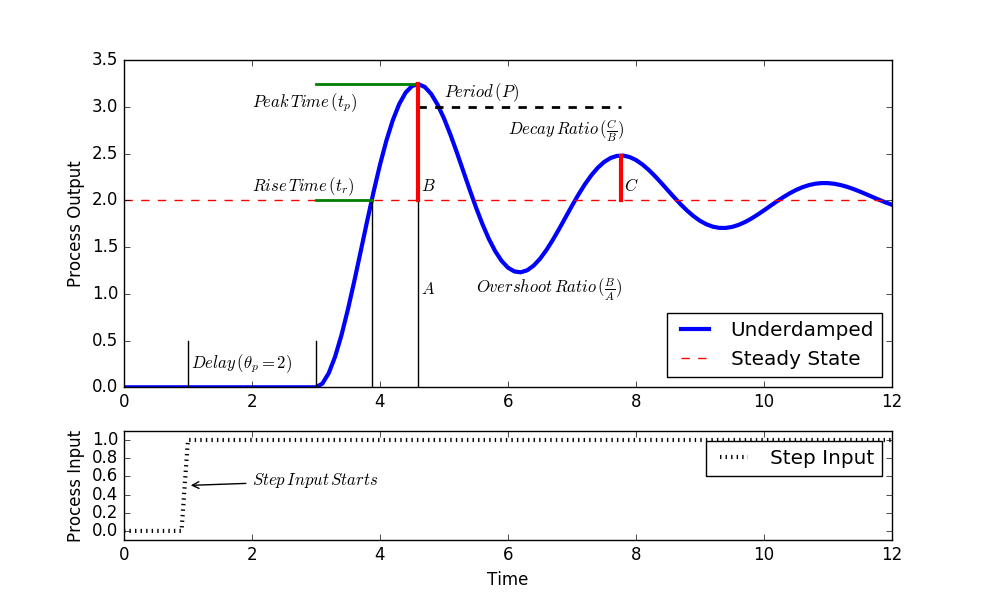
\includegraphics[width=\linewidth]{Images/second_order_graphical_fit.png}
    \caption{Step response of a second order transfer function}
    \label{fig:2nd order step}
\end{figure}
\todo{Redo this figure myself}

A list of the time domain specifications in terms of the canonical variables is shown below:
\begin{align}
     M_p&=  \exp(-\pi\zeta/\sqrt{1-\zeta^2})\\
     t_s(2\%)&= \frac{4}{\sigma}\\
     t_p&=\frac{\pi}{\omega_n\sqrt{1-\zeta^2}}\\
     t_r&=\frac{\pi-\cos^{-1}(\zeta)}{\omega_n\sqrt{1-\zeta^2}}
\end{align}

\subsection{Higher Order Systems}
Very often, our system will have 3 or more poles. In this case, the first or second order descriptions will not be exactly correct. However, it is the case that we can always combine the response of the first and second order systems in order to achieve the same result as a higher order system. Consider a third order system:
$$G_3(s)=\frac{1}{s^3+2s^2+2s+1}$$
We can decompose this system into a first order system and a second order system:
$$G_3(s)=G_1(s)G_2(s)=\frac{K}{s\tau+1}\frac{\omega_n}{s^2+\zeta\omega_ns+\omega_n^2}$$
The appropriate generalization may be done for higher order systems. From here, the exercise becomes an algebraic one. We simply match the terms of the third order polynomial to find the appropriate values. We can start from these conditions (on the numerator and 0th order denominator terms):
\begin{gather}
K\omega_n=1,\quad \omega_n^2=1
\end{gather}
Which make it obvious that both $\omega_n$ and $K$ are necessarily 1. From here, we can expand the rest of the expression:
$$G_3(s)=\frac{1}{s^3+2s^2+s+1}=\frac{1}{\tau s^3+\zeta\tau s^2+s\tau +s^2+\zeta s+1}$$
And we find the following relations:
\begin{gather}
    \tau s^3=s^3\rightarrow\tau=1\\
    2s^2=s^2(\zeta\tau+1)\rightarrow\zeta=1
\end{gather}
This exact approach will not now always work. In general, we require that we have as many degrees of freedom as the number of poles in the system. In general, we would generate a polynomial of the form:
$$\frac{1}{(s+a)(s^2+bs+c)}$$
This factorization may be easily computed with a tool like MATLAB or Python. In MATLAB, we can utilize the following command:
\begin{matlabscript}
syms s
y = s^3+2*s^2+s+1;
factor(y, s, 'FactorMode', 'real')
\end{matlabscript}
Notice that this function does not have a simple factorization like our previous result. MATLAB will return the following:
$$\begin{pmatrix}
s+1.75487 & s^2 +0.24512\,s+0.56984
\end{pmatrix}$$
Now we have values for $a,b$ and $c$ and can construct the appropriate first and second order functions.
\begin{exercise}[Response of Third Order System]
Consider the example above where the third order transfer function takes the form:
$$G(s)=\frac{1}{s^3+2s^2+s+1}$$
We have already shown the factorization can be achieved with MATLAB.
\begin{enumerate}
    \item Find the poles for the second order transfer function of this system
    \item Plot the step response of the first order system, second order system, and third order system on the same plot
\end{enumerate}
\end{exercise}

If you complete the above exercise, you will find that the second order response dominates the response of this system. Why? This occurs because the second order system has its poles closer to the origin. This means that these poles will decay more slowly than the poles further from the origin. As a result, the second order transfer function with the poles closer to the origin will dominate the response of the system. Since the poles are closer to the origin, we call them \textit{dominant} poles of the system.

Often, the true response of our system will have many different modes and be complex. Often we can simplify our system analysis (at least in the beginning) to just include these dominant poles, which will give us a first or second order transfer function which describes the dynamics of the system. This type of reduction is often very useful in flight dynamics systems. If we imagine controlling an aircraft or rocket, there are many modes for a control surface. There may be vibrations in the control surface, various harmonics in the structure, or other high order effects. Typically we can ignore these in control design and consider only the most important delay term(s).

\section{System Type}
Before we actually start designing controllers for systems, we have a few last nuances of transfer functions to cover. The \textit{system type} tells us the polynomial degree of an input where our system has a nonzero constant error. To get started, we need to find the error in our transfer function. If we do the same algebraic analysis as before, we will find that the transfer function from the input to the error is given by:
$$\frac{E(s)}{R(s)}=\frac{1}{1+GH}$$
With a transfer function description of the error, we can use the final value theorem in order to find if the error in the system eventually decreases to zero under a certain input.

To motivate this a bit further, let's consider a simple system with no controller and no feedback. We're going to choose the transfer function of the system to be something simple: $\frac{1}{s+1}$.

\begin{figure}[ht]
    \centering


\tikzset{every picture/.style={line width=0.75pt}} %set default line width to 0.75pt        

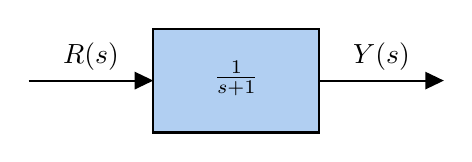
\begin{tikzpicture}[x=0.75pt,y=0.75pt,yscale=-1,xscale=1]
%uncomment if require: \path (0,300); %set diagram left start at 0, and has height of 300

%Flowchart: Process [id:dp22985398749031094] 
\draw  [fill={rgb, 255:red, 74; green, 144; blue, 226 }  ,fill opacity=0.43 ] (280,125) -- (360,125) -- (360,175) -- (280,175) -- cycle ;
%Straight Lines [id:da22245740194670927] 
\draw    (360,150) -- (417,150) ;
\draw [shift={(420,150)}, rotate = 180] [fill={rgb, 255:red, 0; green, 0; blue, 0 }  ][line width=0.08]  [draw opacity=0] (8.93,-4.29) -- (0,0) -- (8.93,4.29) -- cycle    ;
%Straight Lines [id:da8656358522969507] 
\draw    (220,150) -- (277,150) ;
\draw [shift={(280,150)}, rotate = 180] [fill={rgb, 255:red, 0; green, 0; blue, 0 }  ][line width=0.08]  [draw opacity=0] (8.93,-4.29) -- (0,0) -- (8.93,4.29) -- cycle    ;

% Text Node
\draw (250,146.6) node [anchor=south] [inner sep=0.75pt]    {$R( s)$};
% Text Node
\draw (390,146.6) node [anchor=south] [inner sep=0.75pt]    {$Y( s)$};
% Text Node
\draw (320,149) node    {$\frac{1}{s+1}$};


\end{tikzpicture}    
    \caption{Open Loop System Response}
    \label{fig:open loop sys blk diagram}
\end{figure}

When we are concerned with \textit{system type}, we want to know how this system responds to an input of increasing order. When the system is unable to track the input, we know the system type. We'll define a progression of inputs, each of which are the integral of the previous one. We start with the impulse function, $\delta(t)$. As long as our system is stable, it will achieve zero error in response to an impulse response. Integrating the impulse gives the step response, $\frac{1}{s}$ in the Laplace domain. Integrating again gives the ramp response, which is a linearly increasing input. We can keep integrating the input to subject the system to more and more aggressive inputs. The system type is the largest order of input for which a system can achieve zero steady state error. If our system can achieve no steady state error when subjected to a delta function, it is a system type of 0. In response to a step response, it is a system type of 1, and so on.

\begin{example}[Determining system type]
Lets subject the transfer function $\frac{1}{s+2}$ to a step input, which is of the form $\frac{1}{s}$. In the Laplace domain, we have a multiplication:
$$\frac{1}{s(s+2)}$$
We can now apply final value theorem, which will tell us the condition at $t\rightarrow\infty$ since this transfer function is stable:
$$\lim_{s\rightarrow0}\frac{s}{s(s+2)}=\lim_{s\rightarrow0}\frac{1}{s+2}=\frac{1}{2}$$So, we see that when subjected to a unit step, our function eventually reaches the condition that $y(t)=\frac{1}{2}$, not the original input of $1$. So, this function has a steady state error! It will never reach the input condition, no matter how long we wait. Let's now try a ramp input now, which we classify as $\frac{1}{s^2}$. This gives our total function:
$$\frac{1}{s^2(s+1)}$$
and the application of the final value theorem:
$$\lim_{s\rightarrow0}\frac{s}{s^2(s+1)}=\lim_{s\rightarrow0}\frac{1}{s(s+1)}=\infty$$
As we can see, in such a system our final value theorem tells us that such a system will build up infinite error with respect to the ramp input. Finally, let's try the simplest input, the delta function. Since the delta function is simply 1 in the Laplace domain, we apply final value theorem on the original function multiplied by $s$:
$$\lim_{s\rightarrow0}\frac{s}{(s+2)}=0$$
Since the system can only achieve zero steady state error when subjected to the delta function, we say that the system is a type-0 system.
\end{example}

One method of determining system type is to look at the number of `integrators' in the system. That is, we look at how many $\frac{1}{s}$ terms are present in the equation. We can easily tell that the transfer function:
$$G(s)=\frac{3}{s(s+2)}$$
must be a type 1 system because there is one free $\frac{1}{s}$ term. Likewise, the system
$$G(s)=\frac{s^2}{s^4(s+1)}$$
is a type 2 system, because we have $s^2$ in the denominator after the simplification of the rational expression.

The concept of system type tells us one thing that is particularly important. An integrator can reduce or remove steady state error from a system. With that knowledge, we can see why controllers like the PID controller have an `integrator' component. This exists to reduce the steady state error in a system!


\section{Realizing Transfer Functions}

As a last note for this chapter, we should note some of the limitations in writing transfer functions for control systems. 

\subsection{Proper Transfer Functions}
Earlier, we stated that we our concern was mostly with transfer functions that look like:
$$G(s)=\frac{N(s)}{D(s)}=\frac{(s-z_1)(s-z_2)\cdots(s-z_m)}{(s-p_1)(s-p_2)\cdots(s-p_n)}$$
Firstly, we want our transfer functions to be \textit{proper} in almost all cases. This means that the degree of the numerator should be less than or equal to the degree of the denominator ($m\le n$). When this is the case, we call the transfer function proper. The reason for this is somewhat subtle, but it boils down to the fact that no physical system will ever have a numerator with a degree that is greater than the denominator. As an example, let's consider a plant which has an improper transfer function:
$$G(s)=s$$
Of course, this looks like a differentiator in the time domain:
$$g(t)=\frac{du}{dt}$$
For now, we will consider applying no control to the system. We will just subject the system to an impulse function $u=\delta(t)$. The response of the system is the \textit{derivative} of the impulse function!
$$g(t)=\delta'(t)$$
This is obviously nonphysical, it means that output will have an infinite spike. Any improper transfer function will exhibit such behavior. The result is that we do not want such behaviors in physical systems. 

Most of the time, we do not see improper transfer functions arise when we derive systems from correct equations of motion. However, we can see transfer functions that are not \textit{strictly proper}. A strictly proper transfer function is one in which the degree of the numerator is less than the degree of the denominator. However, there is a much easier fix for such systems. We may always write a system where the degree of the numerator and denominator are equal as:
$$G(s)=\frac{(s-z_1)(s-z_2)\cdots(s-z_n)}{(s-p_1)(s-p_2)\cdots(s-p_n)}=\frac{(s-z_1)(s-z_2)\cdots(s-z_{n-1})}{(s-p_1)(s-p_2)\cdots(s-p_n)}+D$$
To actually compute a strictly proper transfer function from a proper one, we use long division.
\begin{example}[Constructing strictly proper transfer functions]

Let's consider the function:
$$G(s)=\frac{s^3+2s^2+1}{s^3+2s}$$ To make such a function strictly proper, we use polynomial long division. We place the numerator inside as the dividend and the denominator as the divisor:
$$\begin{array}{r}
1\phantom{)}   \\
s^3+2s{\overline{\smash{\big)}\,s^2+2s^2+1\phantom{)}}}\\
\underline{-~\phantom{(}(s^3+2s)\phantom{-b)}}\\
2s^2-2s+1\phantom{)}
\end{array}$$
Our final result is the result of the long division with the remainder divided by the original function. Typically, only one step is required to reduce the order sufficiently. In this case, our strictly proper transfer function is:
$$G(s)=\frac{2s^2-2s+1}{s^3+2s}+1$$
\end{example}

\subsection{Rational Transfer Functions}

Our other concern with writing transfer functions is that not all types of functions are represented as polynomial equations. A very common example is a system with delay, where we may have a term like $e^{-st}$ present. Unfortunately, we cannot model such a function using a polynomial equation. Any time we have a function like $\sin(s)$ or $e^{-st}$ present, we cannot use the standard tools of control theory. For delays, this is a big problem! Up until now, we have ignored a pretty crucial part of system dynamics, which is delay. With an ideal transfer function, we don't get any delay in our system dynamics, since our sensors read things off exactly as they happen. This is not a physical reality, though, and we should take a bit of time to consider ways to model systems with delay. While we cannot get exact solutions to such transfer functions, we can approximate them using Pad/'e approximants.

\subsubsection{Pad\'{e} Approximants}

Pad\'e approximants can generally model any function near a specific operating point, but in control theory their primary use is in modeling delays. I will not cover how to calculate the Pad\'e approximant, as the general form can be somewhat intensive. Since a  Pad\'e approximant is a rational polynomial expression, we must define the order of the numerator and denominator. The general form is:
$$\frac{a_0+a_1x+\cdots+a_mx^m}{1+b_1x+b_2x^2+\cdots+b_nx^n}$$
It is required that $m\ge0$ and $n\ge1$. In control theory, we typically also require that the function is proper (though not strictly proper).

In MATLAB, we can use the \texttt{pade} function in two ways. If we are using symbolic variables, it is possible to find the pad\'e approximant of a function \texttt{f} as:
\begin{matlabscript}{Symbolic Pad\'e approximant}
syms x

f = sin(x)

% input function, variable, center point, and order
approxPade = pade(f,x,0,'Order',[3 3])
approxTaylor = taylor(f,x,0,'Order',4)

% plot the result
figure;
fplot(sin(x),[-2,2],'DisplayName', '$\sin(x)$')
hold on
fplot(approxPade,[-2,2], 'DisplayName', 'Pade')
fplot(approxTaylor,[-2,2], 'DisplayName', 'Taylor')
legend(Location="northwest")
title('Comparison of Approximations')
xlabel('$x$')
ylabel('$f(x)$')
    
\end{matlabscript}

We can see that the resulting Pad\'e approximant matches the function much better than the Taylor series as shown in \autoref{fig:taylor v pade}.

\begin{figure}[ht]
    \centering
    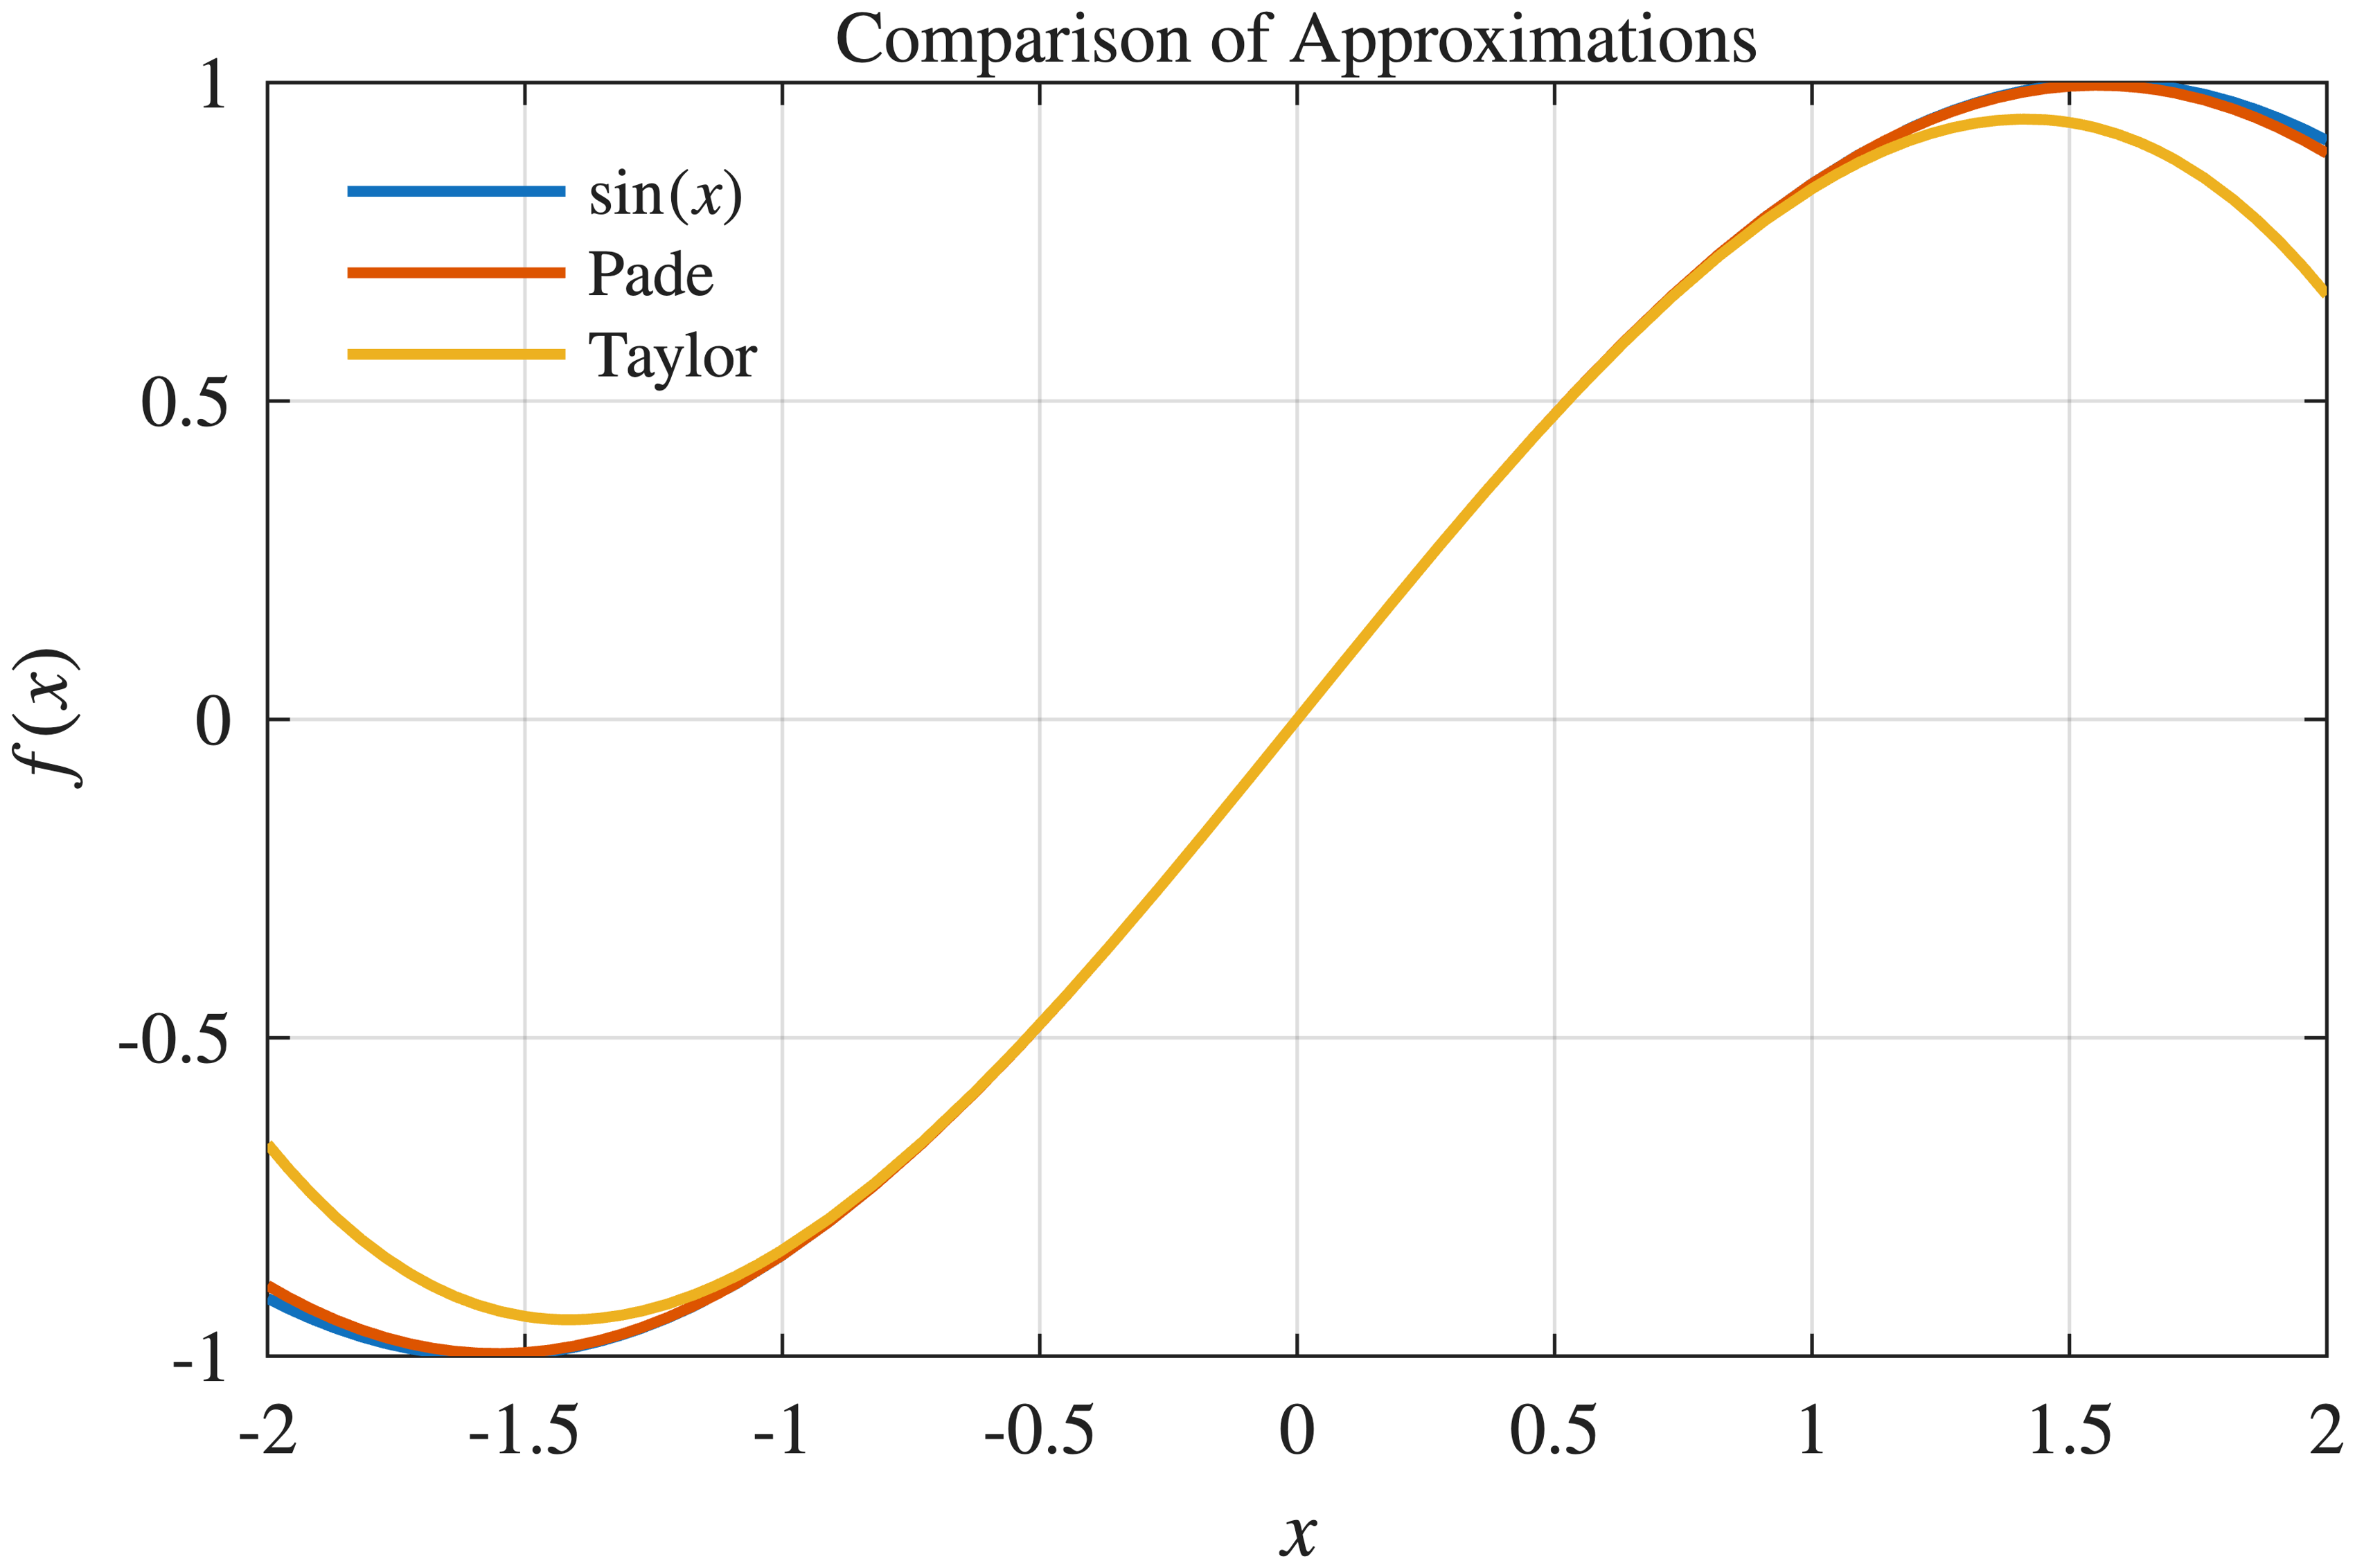
\includegraphics[width=1\linewidth]{ApproximationComp2.png}
    \caption{Comparison of Taylor series and Pad\'e approximations of the sine function}
    \label{fig:taylor v pade}
\end{figure}

This symbolic approach allows us to compute the Pad\'e approximant for an arbitrary functions $f$ (so long as they are analytic around the point of consideration). 

Because we often want to apply the Pad\'e approximant to control systems, MATLAB has a built in function for writing the transfer function of a delay. We use the same function \texttt{pade}, which is interpreted differently when the input is not symbolic. We specify the delay time in seconds and the order of the approximation.
\begin{matlabscript}{Pad\'e approximant for delay}
tau = 0.5;
n = 2;

pade(tau,n)
\end{matlabscript}

This will output a plot showing a true time delay as compared to the Pad/'e approximation, and the phase plot of the true delay as compared to the phase of the approximation (more on this in \autoref{chap:frequency}). The coefficients of the transfer function can be output simply by doing \texttt{[num,den] = pade(tau,n)}.


\section{Practice Problems}

\begin{exercise}[DC Motor]
\begin{enumerate}
    \item Consider a simple control system for a DC motor. The motors angle can be modeled as a simple transfer function between the input voltage $V$ and it's output $\theta$. The controller, $K_p+\frac{K_i}{s}$ is shown to the left of the motor transfer function. This system is shown below in the block diagram in \autoref{fig:motor angle control}:
    \begin{figure}[H]
        \centering
        

\tikzset{every picture/.style={line width=0.75pt}} %set default line width to 0.75pt        

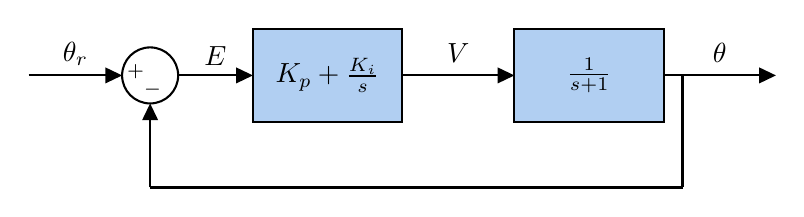
\begin{tikzpicture}[x=0.75pt,y=0.75pt,yscale=-0.9,xscale=0.9]
%uncomment if require: \path (0,300); %set diagram left start at 0, and has height of 300

%Flowchart: Process [id:dp47885050914751914] 
\draw  [fill={rgb, 255:red, 74; green, 144; blue, 226 }  ,fill opacity=0.43 ] (240,145) -- (320,145) -- (320,195) -- (240,195) -- cycle ;
%Flowchart: Process [id:dp27586918225087564] 
\draw  [fill={rgb, 255:red, 74; green, 144; blue, 226 }  ,fill opacity=0.43 ] (380,145) -- (460,145) -- (460,195) -- (380,195) -- cycle ;
%Straight Lines [id:da004910272094030388] 
\draw    (320,170) -- (377,170) ;
\draw [shift={(380,170)}, rotate = 180] [fill={rgb, 255:red, 0; green, 0; blue, 0 }  ][line width=0.08]  [draw opacity=0] (8.93,-4.29) -- (0,0) -- (8.93,4.29) -- cycle    ;
%Straight Lines [id:da2888199737278474] 
\draw    (460,170) -- (517,170) ;
\draw [shift={(520,170)}, rotate = 180] [fill={rgb, 255:red, 0; green, 0; blue, 0 }  ][line width=0.08]  [draw opacity=0] (8.93,-4.29) -- (0,0) -- (8.93,4.29) -- cycle    ;
%Straight Lines [id:da3783579579400398] 
\draw    (120,170) -- (167,170) ;
\draw [shift={(170,170)}, rotate = 180] [fill={rgb, 255:red, 0; green, 0; blue, 0 }  ][line width=0.08]  [draw opacity=0] (8.93,-4.29) -- (0,0) -- (8.93,4.29) -- cycle    ;
%Straight Lines [id:da8246631595636741] 
\draw    (470,170) -- (470,230) ;
%Shape: Circle [id:dp187718705079432] 
\draw   (170,170) .. controls (170,161.72) and (176.72,155) .. (185,155) .. controls (193.28,155) and (200,161.72) .. (200,170) .. controls (200,178.28) and (193.28,185) .. (185,185) .. controls (176.72,185) and (170,178.28) .. (170,170) -- cycle ;
%Straight Lines [id:da23452296039315146] 
\draw    (185,230) -- (185,188) ;
\draw [shift={(185,185)}, rotate = 90] [fill={rgb, 255:red, 0; green, 0; blue, 0 }  ][line width=0.08]  [draw opacity=0] (8.93,-4.29) -- (0,0) -- (8.93,4.29) -- cycle    ;
%Straight Lines [id:da9138966679831894] 
\draw    (185,230) -- (470,230) ;
%Straight Lines [id:da8765530681435604] 
\draw    (200,170) -- (237,170) ;
\draw [shift={(240,170)}, rotate = 180] [fill={rgb, 255:red, 0; green, 0; blue, 0 }  ][line width=0.08]  [draw opacity=0] (8.93,-4.29) -- (0,0) -- (8.93,4.29) -- cycle    ;

% Text Node
\draw (145,166.6) node [anchor=south] [inner sep=0.75pt]    {$\theta _{r}$};
% Text Node
\draw (350,164.6) node [anchor=south] [inner sep=0.75pt]    {$V$};
% Text Node
\draw (490,164.6) node [anchor=south] [inner sep=0.75pt]    {$\theta $};
% Text Node
\draw (171,168) node [anchor=west] [inner sep=0.75pt]  [font=\scriptsize]  {$+$};
% Text Node
\draw (180,177.5) node [anchor=west] [inner sep=0.75pt]  [font=\scriptsize]  {$-$};
% Text Node
\draw (220,166.6) node [anchor=south] [inner sep=0.75pt]    {$E$};
% Text Node
\draw (280,170) node    {$K_{p} +\frac{K_{i}}{s}$};
% Text Node
\draw (420,170) node    {$\frac{1}{s+1}$};


\end{tikzpicture}

        \caption{Motor Angle Control}
        \label{fig:motor angle control}
    \end{figure}
    \begin{enumerate}
        \item Find the open-loop transfer function of the system. This is the transfer function that you would find if the sum block did not have anything being subtracted. Call this transfer function $L(s)$.
        \item Find the closed loop transfer function of the system, given as $\frac{\theta}{\theta_r}$.
        \item Take $K_p=K_i=1$ and $\theta_r=\frac{1}{s}$. What is the final value of $\theta$ as $t\rightarrow\infty$?
        \item Compute $1+L(s)$. How does this compare with the closed loop transfer function that you found?
    \end{enumerate}
\end{enumerate}

\end{exercise}

\newpage
\printendnotes

\chapter{Root Locus Design}\label{chap:root locus}

In our exploration of transfer functions, we discovered that we can change the stability of a system by changing the gain $K$.  This turns out to be very powerful for designing controllers, and we will utilize this capability in our first method of controller design: the \textit{root locus} design method.

With root locus design, we are going to use the pole-zero plot to explore how changing a gain $K$ will alter the pole locations of our function. We look at the locus of all points in the pole-zero plot, given by different values of $K$, which allows us to pick a good value of $K$ to control our system. With this method, we can design a number of controllers, including PID controllers and lead-lag compensators.

\section{Feedback Control}
To design a system via the root locus method, we first need to know what our systems look like. We'll restrict our focus to a few prototypical systems, like shown in \autoref{fig:root locus}.
\begin{figure}[ht]
    \centering



\tikzset{every picture/.style={line width=0.75pt}} %set default line width to 0.75pt        

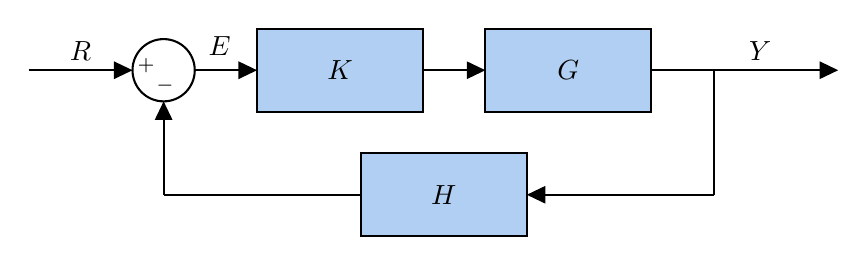
\begin{tikzpicture}[x=0.75pt,y=0.75pt,yscale=-1,xscale=1]
%uncomment if require: \path (0,300); %set diagram left start at 0, and has height of 300

%Flowchart: Process [id:dp1875054016665445] 
\draw  [fill={rgb, 255:red, 74; green, 144; blue, 226 }  ,fill opacity=0.43 ] (370,110) -- (450,110) -- (450,150) -- (370,150) -- cycle ;
%Straight Lines [id:da7499236715272949] 
\draw    (450,130) -- (537,130) ;
\draw [shift={(540,130)}, rotate = 180] [fill={rgb, 255:red, 0; green, 0; blue, 0 }  ][line width=0.08]  [draw opacity=0] (8.93,-4.29) -- (0,0) -- (8.93,4.29) -- cycle    ;
%Straight Lines [id:da8364498609050864] 
\draw    (150,130) -- (197,130) ;
\draw [shift={(200,130)}, rotate = 180] [fill={rgb, 255:red, 0; green, 0; blue, 0 }  ][line width=0.08]  [draw opacity=0] (8.93,-4.29) -- (0,0) -- (8.93,4.29) -- cycle    ;
%Flowchart: Process [id:dp08682453763533549] 
\draw  [fill={rgb, 255:red, 74; green, 144; blue, 226 }  ,fill opacity=0.43 ] (310,170) -- (390,170) -- (390,210) -- (310,210) -- cycle ;
%Straight Lines [id:da254847170018897] 
\draw    (480,130) -- (480,190) ;
%Straight Lines [id:da15845579880945837] 
\draw    (480,190) -- (393,190) ;
\draw [shift={(390,190)}, rotate = 360] [fill={rgb, 255:red, 0; green, 0; blue, 0 }  ][line width=0.08]  [draw opacity=0] (8.93,-4.29) -- (0,0) -- (8.93,4.29) -- cycle    ;
%Shape: Circle [id:dp8927677477080708] 
\draw   (200,130) .. controls (200,121.72) and (206.72,115) .. (215,115) .. controls (223.28,115) and (230,121.72) .. (230,130) .. controls (230,138.28) and (223.28,145) .. (215,145) .. controls (206.72,145) and (200,138.28) .. (200,130) -- cycle ;
%Straight Lines [id:da454001042018386] 
\draw    (215,190) -- (215,148) ;
\draw [shift={(215,145)}, rotate = 90] [fill={rgb, 255:red, 0; green, 0; blue, 0 }  ][line width=0.08]  [draw opacity=0] (8.93,-4.29) -- (0,0) -- (8.93,4.29) -- cycle    ;
%Straight Lines [id:da23591030240460575] 
\draw    (215,190) -- (310,190) ;
%Straight Lines [id:da9810682365957232] 
\draw    (230,130) -- (257,130) ;
\draw [shift={(260,130)}, rotate = 180] [fill={rgb, 255:red, 0; green, 0; blue, 0 }  ][line width=0.08]  [draw opacity=0] (8.93,-4.29) -- (0,0) -- (8.93,4.29) -- cycle    ;
%Flowchart: Process [id:dp6713546674027889] 
\draw  [fill={rgb, 255:red, 74; green, 144; blue, 226 }  ,fill opacity=0.43 ] (260,110) -- (340,110) -- (340,150) -- (260,150) -- cycle ;
%Straight Lines [id:da35454147722483087] 
\draw    (340,130) -- (367,130) ;
\draw [shift={(370,130)}, rotate = 180] [fill={rgb, 255:red, 0; green, 0; blue, 0 }  ][line width=0.08]  [draw opacity=0] (8.93,-4.29) -- (0,0) -- (8.93,4.29) -- cycle    ;

% Text Node
\draw (175,126.6) node [anchor=south] [inner sep=0.75pt]    {$R$};
% Text Node
\draw (502.5,126.6) node [anchor=south] [inner sep=0.75pt]    {$Y$};
% Text Node
\draw (201,128) node [anchor=west] [inner sep=0.75pt]  [font=\scriptsize]  {$+$};
% Text Node
\draw (210,137.5) node [anchor=west] [inner sep=0.75pt]  [font=\scriptsize]  {$-$};
% Text Node
\draw (410,130) node    {$G$};
% Text Node
\draw (350,190) node    {$H$};
% Text Node
\draw (242,124.6) node [anchor=south] [inner sep=0.75pt]    {$E$};
% Text Node
\draw (300,130) node    {$K$};

\end{tikzpicture}
    \caption{Control System for Root Locus Design}
    \label{fig:root locus}
\end{figure}

For simplicity, we'll consider this gain $K$ to be part of the transfer function $G$. I have only written it out explicitly to remind us that it's a variable in our system. From now on, we'll set $G=GK$. We remember that we can understand the transfer function of such a system using the block diagram rules. For the transfer function from $R$ to $Y$, we have:
$$\frac{Y(s)}{R(s)}=\frac{G}{1+GH}$$
And if we wanted to find the error, we could use the relationship that
$$\frac{E(s)}{R(s)}=\frac{1}{1+GH}$$
We notice that this denominator -- $1+GH$ -- is the same for both systems. For root locus design, we consider this denominator so important that we assign some special terminology to it. We call the terms $GH$ the \textit{loop transfer function}, since this is the transfer function that we have before closing the feedback loop. As a shorthand, we give this loop transfer function the variable $L$.\endnote{Unfortunately, there are a great many things in this book which use the letter $L$ or some variation of it. I will try to clarify in the case it is not clear.} We can thus rewrite $1+GH$ as $1+L(s)$.

As we know from our study of transfer functions, the zeros of $1+L(S)$ (the poles of the transfer function) tell us the stability of our system. When we do root locus design, we concern ourselves with this function, $1+L(s)$. Let's remember that we would like $L(s)$ to contain some controller with gain $K$ so that we can change the stability characteristics of our system. Other than this requirement, $L(s)$ can be any proper transfer function. We assume that $L(s)$ is of the form:
$$L(s)=K\frac{(s+z_1)(s+z_2)\cdots(s+z_n)}{(s+p_1)(s+p_2)\cdots(s+p_n)}$$
Our basic equation for root locus design is then just $1+L(s)$, the location of the poles for the closed loop system:
\begin{gather}
    \color{boxBlue}\boxed{\color{black}1+K\frac{(s+z_1)(s+z_2)\cdots(s+z_n)}{(s+p_1)(s+p_2)\cdots(s+p_n)}=0}\\
    \color{boxBlue}\text{Root Locus Equation}
\end{gather}

We're interested in the trajectories of the variable $s$ that solve this equation as we vary the value of $K$. That plot is what we call the root locus of the system.

\section{Basics of Root Locus}
In this text, we won't concern ourselves too heavily with rules for drawing a root locus. In the modern day, you rarely find yourself far from a computer with an install of MATLAB or Python. However, a good control systems engineer should understand how these plots work and be able to draw a basic version of the plot. For that reason we must still cover some of the basic ideas of the root locus.\endnote{Perhaps you would one day like to draw such a plot by hand to impress people who you were friends with before you started talking about control systems. You would be well off to learn how to draw such a plot then!}

\subsubsection{Poles and Zeros}
To get a handle on the root locus, we'll consider the extreme conditions on $K$ first. We typically don't let $K$ be negative, so our smallest condition is when $K\approx0$.\endnote{We have this approximate condition to avoid the singularity when $K=0$ exactly. Notice that if we are not careful with this we would instead find that $1=0$ which is obviously incorrect.} Our other condition is when $K\rightarrow\infty$. Let's see what happens to our root locus equation in those two cases. Let's start with the case where $K\approx0$. We'll start by multiplying our equation by the denominator, $(s+p_1)(s+p_2)\cdots(s+p_n)$, to get
$$(s+p_1)(s+p_2)\cdots(s+p_n)+K(s+z_1)(s+z_2)\cdots(s+z_n)=0$$
When we now set $K\approx0$, we find that the equation looks like:
$$(s+p_1)(s+p_2)\cdots(s+p_n)=0$$
The solutions of this equation are the poles of this equation, $s=-p_1,-p_2\cdots p_n$. We have a simple fact, then, \textbf{that the root locus begins near the open-loop poles}. That is, at zero gain, we expect that our closed loop system will have its poles at the same locations at the poles of the open loop system.

We make a similar argument as $K\rightarrow\infty$. In that case, the poles become inconsequential in compare to the zeros of the function. The function approaches the condition that
$$(s+z_1)(s+z_2)\cdots(s+z_n)=0$$
So, we see that \textbf{the root locus ends near the open-loop zeros}.

The only problem of course, is that not all transfer functions have the same number of poles and zeros. Some of our paths, then, will not follow this behavior. What happens instead is that these poles will `break free' and go off to infinity. We'll see how to deal with those now.

\subsubsection{Constraint Conditions}
Understanding what happens at the extreme conditions of $K$ is not good enough to draw an accurate plot. As a result, we have to introduce some equations of constraint to fully solve our system. As it turns out, that equation of constraint is the same one we've been using this whole time:
$$1+K\frac{(s+z_1)(s+z_2)\cdots(s+z_n)}{(s+p_1)(s+p_2)\cdots(s+p_n)}=0$$
Solving this directly by hand is challenging unless we are clever.\endnote{Luckily, we are very clever.} Instead of solving the equation as presented, we may rearrange it and solve two much simpler problems:
$$K\frac{(s+z_1)(s+z_2)\cdots(s+z_n)}{(s+p_1)(s+p_2)\cdots(s+p_n)}=-1$$
With this new equation, we can see that the magnitude of the LHS of the equation must be $1$, and the angle must be $180\degree$ since $-1$ is rotated $180\degree$ from the positive direction of the real number line.\endnote{It is common in controls to use degrees instead of radians for these measurements. Feel free to use radians and substitute $\pi$ into this equation.} Using this fact, we have two constraint equations:
\begin{gather}
    \left|K\frac{(s+z_1)(s+z_2)\cdots(s+z_n)}{(s+p_1)(s+p_2)\cdots(s+p_n)}\right|=1\\
    \angle{K\frac{(s+z_1)(s+z_2)\cdots(s+z_n)}{(s+p_1)(s+p_2)\cdots(s+p_n)}}=180\degree(2n+1)\quad n=0,\pm1,\pm2,\cdots
\end{gather}
We may also write the second equation in a more digestible form, taking each angle term separately. Remember that we subtract the angle of any poles since they are in the denominator:
$$\angle{(s+z_1)}+\angle{(s+z_2)}+\cdots\angle{(s+z_n)-\angle(s+p_1)-\angle(s+p_2)-\cdots=180\degree}$$
These two equations are enough to uniquely determine the trajectory of $s$, since the values of $z$ and $p$ are known, leaving us with just two variables in $K$ and $s$.

Once again, we could solve these equations directly, but we'll instead come up with a few rules that make our lives a bit easier. Every rule we create will come from these two basic equations, though, so we can always fall back to the simple approach of computing solutions this way. When a computer draws a root locus, it essentially solves these equations for a large number of points to display the result to you.

\section{Drawing Rules for Root Locus}
Using the two equations we described above, we can come up with a few basic rules for drawing the root locus diagram. These will be helpful for drawing the root locus by hand, but they aren't enough to always draw a perfectly accurate system for more complex transfer functions.
\subsection{Real axis values}
Starting with the points on the real axis of the root locus is a very easy starting point. Any point on real axis will have an angle of either $0\degree$ or $180\degree$ with respect to other points on the real axis, so we can quite easily find the lines which satisfy the angle condition. Let's consider a simple system with the transfer function and draw it's pole-zero plot:
$$L(s)=\frac{K}{s(s+2)(s+4)}$$

\begin{figure}[ht]
    \centering



\tikzset{every picture/.style={line width=0.75pt}} %set default line width to 0.75pt        

\begin{tikzpicture}[x=0.75pt,y=0.75pt,yscale=-1,xscale=1]
%uncomment if require: \path (0,300); %set diagram left start at 0, and has height of 300

%Straight Lines [id:da4592564061031674] 
\draw    (330,85) -- (330,195) ;
%Straight Lines [id:da9963825813428108] 
\draw    (410,140) -- (200,140) ;
%Straight Lines [id:da6649082888514012] 
\draw [color={rgb, 255:red, 218; green, 44; blue, 0 }  ,draw opacity=1 ]   (330,140) ;
\draw [shift={(330,140)}, rotate = 45] [color={rgb, 255:red, 218; green, 44; blue, 0 }  ,draw opacity=1 ][line width=0.75]    (-5.59,0) -- (5.59,0)(0,5.59) -- (0,-5.59)   ;
%Straight Lines [id:da6127406045364459] 
\draw    (290,135) -- (290,145) ;
%Straight Lines [id:da6042218853244153] 
\draw    (310,135) -- (310,145) ;
%Straight Lines [id:da4724858061335113] 
\draw    (270,135) -- (270,145) ;
%Straight Lines [id:da9072493933623741] 
\draw    (250,135) -- (250,145) ;
%Straight Lines [id:da3451637976960903] 
\draw    (210,135) -- (210,145) ;
%Straight Lines [id:da5828238919882395] 
\draw    (230,135) -- (230,145) ;
%Straight Lines [id:da13765840163046827] 
\draw [color={rgb, 255:red, 218; green, 44; blue, 0 }  ,draw opacity=1 ][line width=0.75]    (250,140) ;
\draw [shift={(250,140)}, rotate = 45] [color={rgb, 255:red, 218; green, 44; blue, 0 }  ,draw opacity=1 ][line width=0.75]    (-5.59,0) -- (5.59,0)(0,5.59) -- (0,-5.59)   ;
%Straight Lines [id:da5582241552813054] 
\draw [color={rgb, 255:red, 218; green, 44; blue, 0 }  ,draw opacity=1 ]   (290,140) ;
\draw [shift={(290,140)}, rotate = 45] [color={rgb, 255:red, 218; green, 44; blue, 0 }  ,draw opacity=1 ][line width=0.75]    (-5.59,0) -- (5.59,0)(0,5.59) -- (0,-5.59)   ;

% Text Node
\draw (376,62.4) node [anchor=north west][inner sep=0.75pt]    {$\mathbb{C}$};
% Text Node
\draw (217,102.4) node [anchor=north west][inner sep=0.75pt]  [color={rgb, 255:red, 74; green, 144; blue, 226 }  ,opacity=1 ]  {$1$};
% Text Node
\draw (265,102.4) node [anchor=north west][inner sep=0.75pt]  [color={rgb, 255:red, 74; green, 144; blue, 226 }  ,opacity=1 ]  {$2$};
% Text Node
\draw (307,102.4) node [anchor=north west][inner sep=0.75pt]  [color={rgb, 255:red, 74; green, 144; blue, 226 }  ,opacity=1 ]  {$3$};
% Text Node
\draw (347,102.4) node [anchor=north west][inner sep=0.75pt]  [color={rgb, 255:red, 74; green, 144; blue, 226 }  ,opacity=1 ]  {$4$};


\end{tikzpicture}


    \caption{Pole-Zero plot for $\frac{K}{s(s+2)(s+4)}$}
    \label{fig:pole zero real line}
\end{figure}
I've labeled each region of this graph $1-4$ so they can be discussed easily. Let's start with region $1$ and place a test point on the real line:
\begin{figure}[ht]
    \centering



\tikzset{every picture/.style={line width=0.75pt}} %set default line width to 0.75pt        

\begin{tikzpicture}[x=0.75pt,y=0.75pt,yscale=-1,xscale=1]
%uncomment if require: \path (0,300); %set diagram left start at 0, and has height of 300

%Straight Lines [id:da42234123482759833] 
\draw    (350,105) -- (350,215) ;
%Straight Lines [id:da6312770408796599] 
\draw    (430,160) -- (220,160) ;
%Straight Lines [id:da3991094241368439] 
\draw [color={rgb, 255:red, 218; green, 44; blue, 0 }  ,draw opacity=1 ]   (350,160) ;
\draw [shift={(350,160)}, rotate = 45] [color={rgb, 255:red, 218; green, 44; blue, 0 }  ,draw opacity=1 ][line width=0.75]    (-5.59,0) -- (5.59,0)(0,5.59) -- (0,-5.59)   ;
%Straight Lines [id:da8930512815405481] 
\draw    (310,155) -- (310,165) ;
%Straight Lines [id:da9891327275884197] 
\draw    (330,155) -- (330,165) ;
%Straight Lines [id:da977564124434322] 
\draw    (290,155) -- (290,165) ;
%Straight Lines [id:da2628578582402691] 
\draw    (270,155) -- (270,165) ;
%Straight Lines [id:da01003950309758983] 
\draw    (230,155) -- (230,165) ;
%Straight Lines [id:da2824780370007598] 
\draw    (250,155) -- (250,165) ;
%Straight Lines [id:da6956366343677244] 
\draw [color={rgb, 255:red, 218; green, 44; blue, 0 }  ,draw opacity=1 ][line width=0.75]    (270,160) ;
\draw [shift={(270,160)}, rotate = 45] [color={rgb, 255:red, 218; green, 44; blue, 0 }  ,draw opacity=1 ][line width=0.75]    (-5.59,0) -- (5.59,0)(0,5.59) -- (0,-5.59)   ;
%Straight Lines [id:da8951560250601152] 
\draw [color={rgb, 255:red, 218; green, 44; blue, 0 }  ,draw opacity=1 ]   (310,160) ;
\draw [shift={(310,160)}, rotate = 45] [color={rgb, 255:red, 218; green, 44; blue, 0 }  ,draw opacity=1 ][line width=0.75]    (-5.59,0) -- (5.59,0)(0,5.59) -- (0,-5.59)   ;
%Straight Lines [id:da08754341599231841] 
\draw [color={rgb, 255:red, 126; green, 211; blue, 33 }  ,draw opacity=1 ]   (240,160) ;
\draw [shift={(240,160)}, rotate = 0] [color={rgb, 255:red, 126; green, 211; blue, 33 }  ,draw opacity=1 ][fill={rgb, 255:red, 126; green, 211; blue, 33 }  ,fill opacity=1 ][line width=0.75]      (0, 0) circle [x radius= 2.01, y radius= 2.01]   ;

% Text Node
\draw (396,82.4) node [anchor=north west][inner sep=0.75pt]    {$\mathbb{C}$};
% Text Node
\draw (237,122.4) node [anchor=north west][inner sep=0.75pt]  [color={rgb, 255:red, 74; green, 144; blue, 226 }  ,opacity=1 ]  {$1$};
% Text Node
\draw (285,122.4) node [anchor=north west][inner sep=0.75pt]  [color={rgb, 255:red, 74; green, 144; blue, 226 }  ,opacity=1 ]  {$2$};
% Text Node
\draw (327,122.4) node [anchor=north west][inner sep=0.75pt]  [color={rgb, 255:red, 74; green, 144; blue, 226 }  ,opacity=1 ]  {$3$};
% Text Node
\draw (367,122.4) node [anchor=north west][inner sep=0.75pt]  [color={rgb, 255:red, 74; green, 144; blue, 226 }  ,opacity=1 ]  {$4$};


\end{tikzpicture}


    \caption{Pole-Zero plot with test point in region 1}
    \label{fig:real line test point}
\end{figure}
The magnitude condition in this case is trivial. Given that $s$ is a real number, we can see that the transfer function takes the form:
$$\left|\frac{K}{\text{real number}}\right|=1$$
By varying $K$, it should be apparent that we can reach any point along the real number line. We simply let $K$ be equal to the number in question (or it's negative). The angle condition is more interesting. We consider the angle from each pole to our test point. Starting at point $1$, we see that the angle from the pole at $s+4$ is straight behind at $180\degree$. At $s+2$, the angle is once again $180\degree$.  At $s$, the same is of course true. Altogether, we have that the angle is:\endnote{If you are confused about the presence of minus signs in this equation, note that an angle in the denominator of a transfer function is subtracted from the angle total. Notice also that I wrapped the angle $-540\degree$ to $180\degree$ since they are equivalent.}
$$-\angle s-\angle s+2 - \angle s+4 =-180\degree-180\degree-180\degree=180\degree$$
Notice that we did not need to specify \textit{where} in region $1$ that the test point was. It was a general fact that the angle in this region was always $180\degree$, so it holds that for all $s$ in region $1$, the angle condition is satisfied. Let's update our picture, filling in that region, and move to region $2$.
\begin{figure}[ht]
    \centering



\tikzset{every picture/.style={line width=0.75pt}} %set default line width to 0.75pt        

\begin{tikzpicture}[x=0.75pt,y=0.75pt,yscale=-1,xscale=1]
%uncomment if require: \path (0,300); %set diagram left start at 0, and has height of 300

%Straight Lines [id:da1075253924249302] 
\draw    (370,125) -- (370,235) ;
%Straight Lines [id:da6436891349755611] 
\draw    (450,180) -- (240,180) ;
%Straight Lines [id:da9588796525597767] 
\draw [color={rgb, 255:red, 218; green, 44; blue, 0 }  ,draw opacity=1 ]   (370,180) ;
\draw [shift={(370,180)}, rotate = 45] [color={rgb, 255:red, 218; green, 44; blue, 0 }  ,draw opacity=1 ][line width=0.75]    (-5.59,0) -- (5.59,0)(0,5.59) -- (0,-5.59)   ;
%Straight Lines [id:da6480406030877912] 
\draw    (330,175) -- (330,185) ;
%Straight Lines [id:da1577577240172655] 
\draw    (350,175) -- (350,185) ;
%Straight Lines [id:da10491033624249835] 
\draw    (310,175) -- (310,185) ;
%Straight Lines [id:da7331758214772246] 
\draw    (290,175) -- (290,185) ;
%Straight Lines [id:da43740177872716535] 
\draw    (250,175) -- (250,185) ;
%Straight Lines [id:da2679503792515793] 
\draw    (270,175) -- (270,185) ;
%Straight Lines [id:da27022016217643263] 
\draw [color={rgb, 255:red, 218; green, 44; blue, 0 }  ,draw opacity=1 ][line width=0.75]    (290,180) ;
\draw [shift={(290,180)}, rotate = 45] [color={rgb, 255:red, 218; green, 44; blue, 0 }  ,draw opacity=1 ][line width=0.75]    (-5.59,0) -- (5.59,0)(0,5.59) -- (0,-5.59)   ;
%Straight Lines [id:da8099213596250292] 
\draw [color={rgb, 255:red, 218; green, 44; blue, 0 }  ,draw opacity=1 ]   (330,180) ;
\draw [shift={(330,180)}, rotate = 45] [color={rgb, 255:red, 218; green, 44; blue, 0 }  ,draw opacity=1 ][line width=0.75]    (-5.59,0) -- (5.59,0)(0,5.59) -- (0,-5.59)   ;
%Straight Lines [id:da535188488118251] 
\draw [color={rgb, 255:red, 126; green, 211; blue, 33 }  ,draw opacity=1 ]   (310,180) ;
\draw [shift={(310,180)}, rotate = 0] [color={rgb, 255:red, 126; green, 211; blue, 33 }  ,draw opacity=1 ][fill={rgb, 255:red, 126; green, 211; blue, 33 }  ,fill opacity=1 ][line width=0.75]      (0, 0) circle [x radius= 2.01, y radius= 2.01]   ;
%Straight Lines [id:da524021046009422] 
\draw [color={rgb, 255:red, 218; green, 44; blue, 0 }  ,draw opacity=1 ][line width=1.5]    (234,180) -- (290,180) ;
\draw [shift={(230,180)}, rotate = 0] [fill={rgb, 255:red, 218; green, 44; blue, 0 }  ,fill opacity=1 ][line width=0.08]  [draw opacity=0] (9.29,-4.46) -- (0,0) -- (9.29,4.46) -- cycle    ;

% Text Node
\draw (416,102.4) node [anchor=north west][inner sep=0.75pt]    {$\mathbb{C}$};
% Text Node
\draw (257,142.4) node [anchor=north west][inner sep=0.75pt]  [color={rgb, 255:red, 74; green, 144; blue, 226 }  ,opacity=1 ]  {$1$};
% Text Node
\draw (305,142.4) node [anchor=north west][inner sep=0.75pt]  [color={rgb, 255:red, 74; green, 144; blue, 226 }  ,opacity=1 ]  {$2$};
% Text Node
\draw (347,142.4) node [anchor=north west][inner sep=0.75pt]  [color={rgb, 255:red, 74; green, 144; blue, 226 }  ,opacity=1 ]  {$3$};
% Text Node
\draw (387,142.4) node [anchor=north west][inner sep=0.75pt]  [color={rgb, 255:red, 74; green, 144; blue, 226 }  ,opacity=1 ]  {$4$};


\end{tikzpicture}    
    \caption{Pole-Zero plot with test point in region 2}
    \label{fig:real line region 2}
\end{figure}

I've included a directionality to the arrow in the first region because we know that the root locus starts at the poles, so it must be going towards negative infinity as the gain $K$ is increased. With the new diagram, we can make a similar argument. Notice now that the angle from $s+4$ to the test point is now $0\degree$, not $180\degree$. The others remain the same. In this region, we have:
$$-\angle s-\angle s+2 - \angle s+4 =-180\degree-180\degree-0\degree=0\degree$$
This angle is in violation of the angle constraint, so we learn that there exists no part of the root locus in region $2$. We'll continue similarly with our analysis in regions $3$ and $4$, and we can see that the final result is:
\begin{figure}[ht]
    \centering
    

\tikzset{every picture/.style={line width=0.75pt}} %set default line width to 0.75pt        

\begin{tikzpicture}[x=0.75pt,y=0.75pt,yscale=-1,xscale=1]
%uncomment if require: \path (0,300); %set diagram left start at 0, and has height of 300

%Straight Lines [id:da3483152737455598] 
\draw    (390,145) -- (390,255) ;
%Straight Lines [id:da016062354812395263] 
\draw    (470,200) -- (260,200) ;
%Straight Lines [id:da44157825315764965] 
\draw [color={rgb, 255:red, 218; green, 44; blue, 0 }  ,draw opacity=1 ]   (390,200) ;
\draw [shift={(390,200)}, rotate = 45] [color={rgb, 255:red, 218; green, 44; blue, 0 }  ,draw opacity=1 ][line width=0.75]    (-5.59,0) -- (5.59,0)(0,5.59) -- (0,-5.59)   ;
%Straight Lines [id:da7286719847529227] 
\draw    (350,195) -- (350,205) ;
%Straight Lines [id:da41297236301251694] 
\draw    (370,195) -- (370,205) ;
%Straight Lines [id:da2928419898249093] 
\draw    (330,195) -- (330,205) ;
%Straight Lines [id:da11842026013785989] 
\draw    (310,195) -- (310,205) ;
%Straight Lines [id:da4291995443171389] 
\draw    (270,195) -- (270,205) ;
%Straight Lines [id:da1409552586415992] 
\draw    (290,195) -- (290,205) ;
%Straight Lines [id:da4460829576806987] 
\draw [color={rgb, 255:red, 218; green, 44; blue, 0 }  ,draw opacity=1 ][line width=0.75]    (310,200) ;
\draw [shift={(310,200)}, rotate = 45] [color={rgb, 255:red, 218; green, 44; blue, 0 }  ,draw opacity=1 ][line width=0.75]    (-5.59,0) -- (5.59,0)(0,5.59) -- (0,-5.59)   ;
%Straight Lines [id:da8468637902059643] 
\draw [color={rgb, 255:red, 218; green, 44; blue, 0 }  ,draw opacity=1 ]   (350,200) ;
\draw [shift={(350,200)}, rotate = 45] [color={rgb, 255:red, 218; green, 44; blue, 0 }  ,draw opacity=1 ][line width=0.75]    (-5.59,0) -- (5.59,0)(0,5.59) -- (0,-5.59)   ;
%Straight Lines [id:da8631232482140341] 
\draw [color={rgb, 255:red, 218; green, 44; blue, 0 }  ,draw opacity=1 ][line width=1.5]    (254,200) -- (310,200) ;
\draw [shift={(250,200)}, rotate = 0] [fill={rgb, 255:red, 218; green, 44; blue, 0 }  ,fill opacity=1 ][line width=0.08]  [draw opacity=0] (9.29,-4.46) -- (0,0) -- (9.29,4.46) -- cycle    ;
%Straight Lines [id:da3973491588976733] 
\draw [color={rgb, 255:red, 218; green, 44; blue, 0 }  ,draw opacity=1 ][line width=1.5]    (350,200) -- (390,200) ;

% Text Node
\draw (436,122.4) node [anchor=north west][inner sep=0.75pt]    {$\mathbb{C}$};
% Text Node
\draw (277,162.4) node [anchor=north west][inner sep=0.75pt]  [color={rgb, 255:red, 74; green, 144; blue, 226 }  ,opacity=1 ]  {$1$};
% Text Node
\draw (325,162.4) node [anchor=north west][inner sep=0.75pt]  [color={rgb, 255:red, 74; green, 144; blue, 226 }  ,opacity=1 ]  {$2$};
% Text Node
\draw (367,162.4) node [anchor=north west][inner sep=0.75pt]  [color={rgb, 255:red, 74; green, 144; blue, 226 }  ,opacity=1 ]  {$3$};
% Text Node
\draw (407,162.4) node [anchor=north west][inner sep=0.75pt]  [color={rgb, 255:red, 74; green, 144; blue, 226 }  ,opacity=1 ]  {$4$};


\end{tikzpicture}
    \caption{Root locus for real axis poles}
    \label{fig:completed rl real}
\end{figure}

By going through this exercise, we can see that a general pattern emerges. Whenever we have poles on the real axis of our transfer function, \textbf{we know the root locus must be filled in the regions of the real line where there are an odd number of points to the right} (An even number of points to the left gives the same result).

\subsection{Asymptotes}

When we have a greater number of poles than zeros, our root locus will have some parts that go off towards infinity in some direction. Now, we'll figure out how we can find those points.

Our main tool in doing this will be the angle constraint. Let's remember that we can express the angle of the transfer function with
$$\angle G(s)=\angle\text{zeros}-\angle\text{poles}$$
The angles of the asymptotes, then, are related to the number of poles and zeros in our system\footnote{You may find a more in depth derivation at \cite{peet_root_nodate}. I don't cover it deeply here.}.  We denote the number of poles as $P$ and the number of zeros as $Z$. We can denote the center and the angle of the asymptotes as:
\begin{gather}
    \text{Center}: S=\frac{\sum p_i-\sum z_i}{P-Z}\\
    \text{Angle}: \phi=\frac{180\degree(2n+1)}{P-Z} 
\end{gather}

For the center, the equation will vary by a minus sign depending on whether we consider the equation as $(s+p_1)$ or $(s-p_1)$ for the sign convention. Here we choose the former. Ultimately, remember that this location is the average of the `excess' poles. For a stable system, excess poles will always put the center in the left half plane.
\begin{exercise}[Asymptote Angles]\label{exer:asmypote_angle}
Find the center and the asymptote angles for the following transfer functions:
\begin{enumerate}
    \item $G(s)=\frac{s+1}{(s+1)(s+2)}$
    \item $G(s)=\frac{s^2+1}{s^3+10s^2+31s_30}$
    \item This one is (s+2)(s+3)(s+5) for future me
    \item $G(s)=\frac{1}{s+3}$
    \item $G(s)=\frac{1}{s(s+2)(s+4)}$
\end{enumerate}
\end{exercise}

\todo{answers for these}

\subsection{Breakaway points}
Let's return to our example transfer function $L(s)=\frac{K}{s(s+2)(s+4)}$. There, we saw that the real axis region went between two poles (see \autoref{fig:completed rl real}). We know, however, that the root locus should end at a zero or infinity. Therefore, the two poles in this region must escape to infinity at some point in region 3, since there are no zeros. We call this areas where the split occurs a \textit{breakaway point}. At the point where this breakaway occurs, there must be a repeated root (because the two poles meet here for a specific gain $K$ before diverging off to infinity). Let's look for the point where:
$$1+K\frac{N(s)}{D(s)}=0$$ has a repeated root at our test point $s=s^*$. Since we know that this will have a repeated root for $s^*$, we may equivalently state that
\begin{equation}\label{eq:breakaway}
f(s)=D(s)+KN(s)
\end{equation}
has multiple roots. We can equivalently say that the derivative of $f$ at this point must be zero (a proof of this fact can be found in \autoref{multiple root} of the Appendix).
$$f'(s)\bigg\vert_{s=s^*}=D'(s)+KN'(s)\bigg\vert_{s=s^*}=0$$
We can rearrange this statement to the following:
$$K=-\frac{D'(s^*)}{N'(s^*)}$$
Now that we have $K$  in terms of $D'$ and $N'$, we are ready to proceed. Plugging back in to the equation for $f(s)$:
$$D(s^*)-\frac{D'(s^*)}{N'(s^*)}N(s^*)=0$$
We may multiply both sides by $N'(s^*)$ and divide by  $N^2(s^*)$ to get the equation into a recognizable form:
$$\frac{N'(s^*)D(s^*)-D'(s^*)N(s^*)}{N^2(s^*)}=0$$
You will notice that this is the quotient rule for the term $K$. We therefore know that the candidate breakaway points occur for the condition:
$$\frac{dK}{ds}=0$$
We can also rearrange \eqautoref{eq:breakaway} to find another expression for $K$:
$$K=\frac{D(s^*)}{N(s^*)}$$
Let's return to our example in the previous section and add this breakaway point.
\begin{example}[Breakaway points]
We'll again consider the transfer function of the open loop system:
$$L(s)=\frac{K}{s(s+2)(s+4)}$$

We'll remember that we can use the real axis rules to get to the following:

\begin{figure}[H]
    \centering
    


\tikzset{every picture/.style={line width=0.75pt}} %set default line width to 0.75pt        

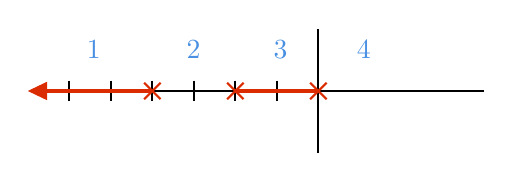
\begin{tikzpicture}[x=0.75pt,y=0.75pt,yscale=-1,xscale=1]
%uncomment if require: \path (0,300); %set diagram left start at 0, and has height of 300

%Straight Lines [id:da7239865282030291] 
\draw    (410,210) -- (410,150) ;
%Straight Lines [id:da6590730859258374] 
\draw    (490,180) -- (280,180) ;
%Straight Lines [id:da5091559258547715] 
\draw [color={rgb, 255:red, 218; green, 44; blue, 0 }  ,draw opacity=1 ]   (410,180) ;
\draw [shift={(410,180)}, rotate = 45] [color={rgb, 255:red, 218; green, 44; blue, 0 }  ,draw opacity=1 ][line width=0.75]    (-5.59,0) -- (5.59,0)(0,5.59) -- (0,-5.59)   ;
%Straight Lines [id:da09618136474024441] 
\draw    (370,175) -- (370,185) ;
%Straight Lines [id:da046174109841857325] 
\draw    (390,175) -- (390,185) ;
%Straight Lines [id:da7153226717951933] 
\draw    (350,175) -- (350,185) ;
%Straight Lines [id:da17390657408205512] 
\draw    (330,175) -- (330,185) ;
%Straight Lines [id:da8694280773997596] 
\draw    (290,175) -- (290,185) ;
%Straight Lines [id:da8677467003751472] 
\draw    (310,175) -- (310,185) ;
%Straight Lines [id:da4266167310519544] 
\draw [color={rgb, 255:red, 218; green, 44; blue, 0 }  ,draw opacity=1 ][line width=0.75]    (330,180) ;
\draw [shift={(330,180)}, rotate = 45] [color={rgb, 255:red, 218; green, 44; blue, 0 }  ,draw opacity=1 ][line width=0.75]    (-5.59,0) -- (5.59,0)(0,5.59) -- (0,-5.59)   ;
%Straight Lines [id:da4164600053953833] 
\draw [color={rgb, 255:red, 218; green, 44; blue, 0 }  ,draw opacity=1 ]   (370,180) ;
\draw [shift={(370,180)}, rotate = 45] [color={rgb, 255:red, 218; green, 44; blue, 0 }  ,draw opacity=1 ][line width=0.75]    (-5.59,0) -- (5.59,0)(0,5.59) -- (0,-5.59)   ;
%Straight Lines [id:da5262888451847954] 
\draw [color={rgb, 255:red, 218; green, 44; blue, 0 }  ,draw opacity=1 ][line width=1.5]    (274,180) -- (330,180) ;
\draw [shift={(270,180)}, rotate = 0] [fill={rgb, 255:red, 218; green, 44; blue, 0 }  ,fill opacity=1 ][line width=0.08]  [draw opacity=0] (9.29,-4.46) -- (0,0) -- (9.29,4.46) -- cycle    ;
%Straight Lines [id:da34588127067625074] 
\draw [color={rgb, 255:red, 218; green, 44; blue, 0 }  ,draw opacity=1 ][line width=1.5]    (370,180) -- (410,180) ;

% Text Node
\draw (297,154.4) node [anchor=north west][inner sep=0.75pt]  [color={rgb, 255:red, 74; green, 144; blue, 226 }  ,opacity=1 ]  {$1$};
% Text Node
\draw (345,154.4) node [anchor=north west][inner sep=0.75pt]  [color={rgb, 255:red, 74; green, 144; blue, 226 }  ,opacity=1 ]  {$2$};
% Text Node
\draw (387,154.4) node [anchor=north west][inner sep=0.75pt]  [color={rgb, 255:red, 74; green, 144; blue, 226 }  ,opacity=1 ]  {$3$};
% Text Node
\draw (427,154.4) node [anchor=north west][inner sep=0.75pt]  [color={rgb, 255:red, 74; green, 144; blue, 226 }  ,opacity=1 ]  {$4$};


\end{tikzpicture}

    \caption{Root locus for real axis poles}
    \label{fig:completed rl real 2}
\end{figure}

Now, our goal is to find the breakaway point. We have already determined this point must be in region 3, but we do not know the exact location yet. Using $\frac{dK}{ds}=0$ we find that:
$$K(s)=-(s^3-6s^2+8s)$$
$$\frac{dK}{ds}=-3s^2-12s-8=0$$
We can solve this quadratic equation to find the roots are approximately $-3.1547$ and $-0.8453$. Only the second lies within the correct region, so that is the one which will yield the correct breakaway point. From here, we can find the appropriate asymptote angle and center (which the reader has found in \autoref{exer:asmypote_angle}) and draw the root locus:

\begin{figure}[H]
    \centering


\tikzset{every picture/.style={line width=0.75pt}} %set default line width to 0.75pt        

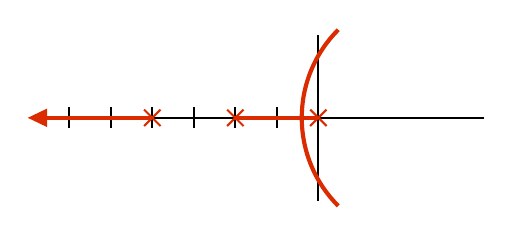
\begin{tikzpicture}[x=0.75pt,y=0.75pt,yscale=-1,xscale=1]
%uncomment if require: \path (0,300); %set diagram left start at 0, and has height of 300

%Straight Lines [id:da7681975539895656] 
\draw    (370,110) -- (370,190) ;
%Straight Lines [id:da7039094827628853] 
\draw    (450,150) -- (240,150) ;
%Straight Lines [id:da16652847971387919] 
\draw [color={rgb, 255:red, 218; green, 44; blue, 0 }  ,draw opacity=1 ]   (370,150) ;
\draw [shift={(370,150)}, rotate = 45] [color={rgb, 255:red, 218; green, 44; blue, 0 }  ,draw opacity=1 ][line width=0.75]    (-5.59,0) -- (5.59,0)(0,5.59) -- (0,-5.59)   ;
%Straight Lines [id:da17992934915470915] 
\draw    (330,145) -- (330,155) ;
%Straight Lines [id:da908519523707048] 
\draw    (350,145) -- (350,155) ;
%Straight Lines [id:da021369612601015775] 
\draw    (310,145) -- (310,155) ;
%Straight Lines [id:da9402916959128319] 
\draw    (290,145) -- (290,155) ;
%Straight Lines [id:da25307127166337107] 
\draw    (250,145) -- (250,155) ;
%Straight Lines [id:da8829008335359465] 
\draw    (270,145) -- (270,155) ;
%Straight Lines [id:da9343756320112938] 
\draw [color={rgb, 255:red, 218; green, 44; blue, 0 }  ,draw opacity=1 ][line width=0.75]    (290,150) ;
\draw [shift={(290,150)}, rotate = 45] [color={rgb, 255:red, 218; green, 44; blue, 0 }  ,draw opacity=1 ][line width=0.75]    (-5.59,0) -- (5.59,0)(0,5.59) -- (0,-5.59)   ;
%Straight Lines [id:da0659337243943724] 
\draw [color={rgb, 255:red, 218; green, 44; blue, 0 }  ,draw opacity=1 ]   (330,150) ;
\draw [shift={(330,150)}, rotate = 45] [color={rgb, 255:red, 218; green, 44; blue, 0 }  ,draw opacity=1 ][line width=0.75]    (-5.59,0) -- (5.59,0)(0,5.59) -- (0,-5.59)   ;
%Straight Lines [id:da21674427210347136] 
\draw [color={rgb, 255:red, 218; green, 44; blue, 0 }  ,draw opacity=1 ][line width=1.5]    (234,150) -- (290,150) ;
\draw [shift={(230,150)}, rotate = 0] [fill={rgb, 255:red, 218; green, 44; blue, 0 }  ,fill opacity=1 ][line width=0.08]  [draw opacity=0] (9.29,-4.46) -- (0,0) -- (9.29,4.46) -- cycle    ;
%Straight Lines [id:da056233766668564056] 
\draw [color={rgb, 255:red, 218; green, 44; blue, 0 }  ,draw opacity=1 ][line width=1.5]    (330,150) -- (370,150) ;
%Shape: Arc [id:dp12422138410800665] 
\draw  [draw opacity=0][line width=1.5]  (379.57,192.43) .. controls (368.72,181.57) and (362,166.57) .. (362,150) .. controls (362,133.43) and (368.72,118.43) .. (379.57,107.57) -- (422,150) -- cycle ; \draw  [color={rgb, 255:red, 218; green, 44; blue, 0 }  ,draw opacity=1 ][line width=1.5]  (379.57,192.43) .. controls (368.72,181.57) and (362,166.57) .. (362,150) .. controls (362,133.43) and (368.72,118.43) .. (379.57,107.57) ;  

\end{tikzpicture}

    \caption{Completed Root Locus}
    \label{fig:root locus break away}
\end{figure}
    
\end{example}
\subsection{Departure and Arrival Angles}
When we have a pole which is not on the real axis, we are not sure of the initial direction in which it will go. To figure this out, we need to consider the angles of the surrounding poles with respect to the given pole, which will dictate the angle at which the pole will start moving as the gain is increased. We add the phase angle of any zeros, and subtract the phase of any poles:
\begin{figure}[ht]
    \centering



\tikzset{every picture/.style={line width=0.75pt}} %set default line width to 0.75pt        

\begin{tikzpicture}[x=0.75pt,y=0.75pt,yscale=-1,xscale=1]
%uncomment if require: \path (0,300); %set diagram left start at 0, and has height of 300

%Straight Lines [id:da9314850339561581] 
\draw [color={rgb, 255:red, 74; green, 144; blue, 226 }  ,draw opacity=1 ]   (420,110) -- (402.12,92.12) ;
\draw [shift={(400,90)}, rotate = 45] [fill={rgb, 255:red, 74; green, 144; blue, 226 }  ,fill opacity=1 ][line width=0.08]  [draw opacity=0] (5.36,-2.57) -- (0,0) -- (5.36,2.57) -- cycle    ;
%Straight Lines [id:da08464605955075277] 
\draw    (470,70) -- (470,230) ;
%Straight Lines [id:da4375711624801496] 
\draw    (520,150) -- (230,150) ;
%Straight Lines [id:da0030428544215852504] 
\draw [color={rgb, 255:red, 218; green, 44; blue, 0 }  ,draw opacity=1 ]   (420,110) ;
\draw [shift={(420,110)}, rotate = 45] [color={rgb, 255:red, 218; green, 44; blue, 0 }  ,draw opacity=1 ][line width=0.75]    (-5.59,0) -- (5.59,0)(0,5.59) -- (0,-5.59)   ;
%Straight Lines [id:da16946530797046677] 
\draw [color={rgb, 255:red, 218; green, 44; blue, 0 }  ,draw opacity=1 ][line width=0.75]    (340,150) ;
\draw [shift={(340,150)}, rotate = 0] [color={rgb, 255:red, 218; green, 44; blue, 0 }  ,draw opacity=1 ][line width=0.75]      (0, 0) circle [x radius= 3.35, y radius= 3.35]   ;
%Straight Lines [id:da8604213500227134] 
\draw [color={rgb, 255:red, 218; green, 44; blue, 0 }  ,draw opacity=1 ]   (420,190) ;
\draw [shift={(420,190)}, rotate = 45] [color={rgb, 255:red, 218; green, 44; blue, 0 }  ,draw opacity=1 ][line width=0.75]    (-5.59,0) -- (5.59,0)(0,5.59) -- (0,-5.59)   ;
%Straight Lines [id:da5601897765807818] 
\draw  [dash pattern={on 0.84pt off 2.51pt}]  (340,150) -- (420,110) ;
%Shape: Arc [id:dp5780263940977343] 
\draw  [draw opacity=0] (369.46,136.26) .. controls (371.41,140.43) and (372.5,145.09) .. (372.5,150) -- (340,150) -- cycle ; \draw    (370.62,139.08) .. controls (371.84,142.5) and (372.5,146.17) .. (372.5,150) ;  \draw [shift={(369.46,136.26)}, rotate = 68.52] [fill={rgb, 255:red, 0; green, 0; blue, 0 }  ][line width=0.08]  [draw opacity=0] (5.36,-2.57) -- (0,0) -- (5.36,2.57) -- cycle    ;
%Straight Lines [id:da8776406333734178] 
\draw  [dash pattern={on 0.84pt off 2.51pt}]  (420,190) -- (436.25,190) ;
%Shape: Arc [id:dp835568621419383] 
\draw  [draw opacity=0] (420.28,173.75) .. controls (429.13,173.9) and (436.25,181.12) .. (436.25,190) .. controls (436.25,190) and (436.25,190) .. (436.25,190) -- (420,190) -- cycle ; \draw    (423.38,174.1) .. controls (430.73,175.66) and (436.25,182.19) .. (436.25,190) ;  \draw [shift={(420.28,173.75)}, rotate = 8.31] [fill={rgb, 255:red, 0; green, 0; blue, 0 }  ][line width=0.08]  [draw opacity=0] (5.36,-2.57) -- (0,0) -- (5.36,2.57) -- cycle    ;
%Shape: Arc [id:dp18314003623219455] 
\draw  [draw opacity=0] (409.13,97.92) .. controls (412.01,95.33) and (415.82,93.75) .. (420,93.75) .. controls (428.97,93.75) and (436.25,101.03) .. (436.25,110) -- (420,110) -- cycle ; \draw    (411.55,96.12) .. controls (414.01,94.61) and (416.91,93.75) .. (420,93.75) .. controls (428.97,93.75) and (436.25,101.03) .. (436.25,110) ;  \draw [shift={(409.13,97.92)}, rotate = 325.13] [fill={rgb, 255:red, 0; green, 0; blue, 0 }  ][line width=0.08]  [draw opacity=0] (5.36,-2.57) -- (0,0) -- (5.36,2.57) -- cycle    ;
%Straight Lines [id:da21143332234166756] 
\draw  [dash pattern={on 0.84pt off 2.51pt}]  (420,190) -- (420,110) ;
%Straight Lines [id:da0892420181184368] 
\draw  [dash pattern={on 0.84pt off 2.51pt}]  (436.25,110) -- (420,110) ;

% Text Node
\draw (378,131.4) node [anchor=north west][inner sep=0.75pt]  [font=\small]  {$\phi $};
% Text Node
\draw (436,165.4) node [anchor=north west][inner sep=0.75pt]  [font=\small]  {$\theta _{1}$};
% Text Node
\draw (431,82.4) node [anchor=north west][inner sep=0.75pt]  [font=\small]  {$\theta _{2}$};


\end{tikzpicture}

    \caption{Determination of the departure angle from the location of poles and zeros}
    \label{fig:root locus departure}
\end{figure}
The resulting constraint for the departure angle is the famililar one:
$$\angle\text{zeros}-\angle\text{poles}=180\degree$$
There is a slight complication if we have coincident poles. A case that we see often is multiple poles at the origin. If we have $M$ such poles with a multiplicity greather than one, we have the following formulas:
\begin{gather}
\text{Angle of Departure from Pole } N:\\
M\theta_N=180\degree -\sum_{i\ne N}\theta_i+\sum_j\phi_i\\
\text{Angle of Arrival at Zero } N:\\
M\phi_N=180\degree -\sum_{i\ne N}\phi_i+\sum_j\theta_i
\end{gather}

And that's basically it! Using these criteria we can draw basic root locus plots. The most important of these to remember are the angle constraints, which we will use when we design controllers via the root locus method. As our root locus plots get more complex, it is hard to predict the behavior using these simple rules. As a result, we often like to compute these numerically.

\todo{Full example here}

\section{Root Locus in Code}
Drawing the root locus with MATLAB or Python is quite simple, but there are a few key points to recognize. First of all, we want our "sys" to be the loop transfer function $L(s)$, not the closed loop system. We may input this in several ways. Typically, we define this "sys" using a transfer function, but we may also input a state space.\endnote{We will discuss state space modeling in later chapters.} For a loop transfer function like:
$$L(s)=K\frac{s+1}{(s+2)(s+4)}$$
We would write the following:
\begin{matlabscript}{}
sys = tf([1 1], [1 6 8])
rlocus(sys)
\end{matlabscript}

The script will automatically draw the associated root locus when called with no outputs like this. However, we can also save the outputs of the rlocus function to plot them in any other way that we like. In Python, we must explicitly plot the output using \texttt{matplotlib}:
\begin{pythonscript}{}
import numpy as np
from matplotlib import pyplot as plt 
import control

G = control.TransferFunction((1, 1), (1, 6, 8))

rlist, klist = control.rlocus(G, gains=np.linspace(0, 10.0, num=1000))

plt.show()
\end{pythonscript}
Both of the scripts above will draw the resulting root locus plot. As practice, you can try drawing the root locus by hand and seeing if it matches the plots you get from running these scripts.

\begin{exercise}[Root Locus Drawings]
    Consider a system with the following loop transfer function:
    $$L(s)=K\frac{s+1}{s(s+2)(s^2+2s+5)}$$
    \begin{enumerate}[label=\alph*)]
        \item Draw the root locus of the system by hand. Calculate the angle of departure and asymptotes for the system
        \item Use MATLAB / Python to verify the root locus for the system
    \end{enumerate}
\end{exercise}

\begin{exercise}[Routh and Root Locus]
Consider a system with the loop transfer function:
$$L(s)=\frac{K(s+1)}{s(s+3)}$$
\begin{enumerate}[label=\alph*)]
\item Determine the closed loop transfer function for the system from the open loop transfer function
\item Use the Routh stability criterion to determine the values of $K$ for which the system is stable.
\item Plot the root locus in MATLAB / Python and show that the $\Im$ axis crossover occurs at the gain $K$ found in part b.
\end{enumerate}
\end{exercise}

\section{Controller Design with Root Locus}
We've now reached a critical point in our journey with control theory. After much background, we're ready to design our first real controller! With some root locus drawing strategies in our toolkit, we can now create controllers which are more complicated that the simple proportional controllers that we could design using the Routh stability criterion. There are a lot of controller designs that are possible using the Root Locus design, but the two most popular and common are PID controllers and lead-lag compensators.

\subsection{PID Control}
The \gls{pid} controller is likely the most popular method for controlling a simple system. The \gls{pid} controller is simple, easily understandable, and has been widely studied due to its early adoption in control theory. The \gls{pid} controller is also quite common because it often requires no knowledge of the system dynamics to set up. Often, the \gls{pid} gains can be found manually through experimentation and requires little analysis. We will investigate these experimental tuning methods in \autoref{chap:inverted pendulum}.

To motivate the \gls{pid} controller, we may consider a `naive' approach to developing a controller. Say we want to develop a cruise control system for a car, which is a classic control system problem. We can represent the control system with a block diagram as shown in \autoref{fig:cruise cont}.

\begin{figure}
    \centering



\tikzset{every picture/.style={line width=0.75pt}} %set default line width to 0.75pt        

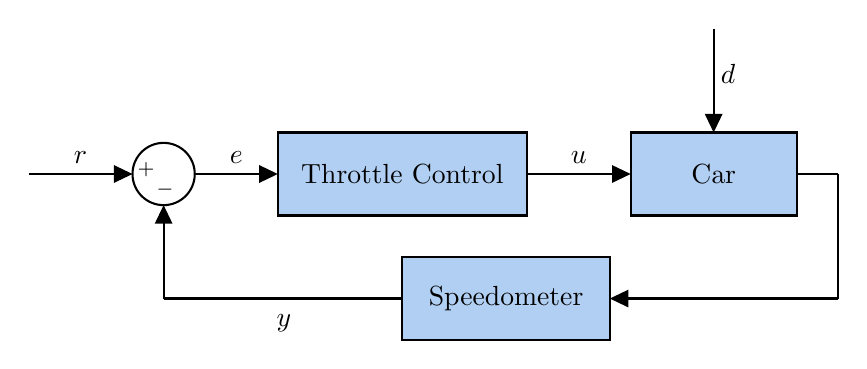
\begin{tikzpicture}[x=0.75pt,y=0.75pt,yscale=-1,xscale=1]
%uncomment if require: \path (0,300); %set diagram left start at 0, and has height of 300

%Flowchart: Process [id:dp09201642540641108] 
\draw  [fill={rgb, 255:red, 74; green, 144; blue, 226 }  ,fill opacity=0.43 ] (220,130) -- (340,130) -- (340,170) -- (220,170) -- cycle ;
%Flowchart: Process [id:dp2324513721050836] 
\draw  [fill={rgb, 255:red, 74; green, 144; blue, 226 }  ,fill opacity=0.43 ] (390,130) -- (470,130) -- (470,170) -- (390,170) -- cycle ;
%Straight Lines [id:da986938021625412] 
\draw    (340,150) -- (387,150) ;
\draw [shift={(390,150)}, rotate = 180] [fill={rgb, 255:red, 0; green, 0; blue, 0 }  ][line width=0.08]  [draw opacity=0] (8.93,-4.29) -- (0,0) -- (8.93,4.29) -- cycle    ;
%Straight Lines [id:da32309733042460087] 
\draw    (470,150) -- (490,150) ;
%Straight Lines [id:da5257263581405386] 
\draw    (100,150) -- (147,150) ;
\draw [shift={(150,150)}, rotate = 180] [fill={rgb, 255:red, 0; green, 0; blue, 0 }  ][line width=0.08]  [draw opacity=0] (8.93,-4.29) -- (0,0) -- (8.93,4.29) -- cycle    ;
%Flowchart: Process [id:dp40423180863818065] 
\draw  [fill={rgb, 255:red, 74; green, 144; blue, 226 }  ,fill opacity=0.43 ] (280,190) -- (380,190) -- (380,230) -- (280,230) -- cycle ;
%Straight Lines [id:da8433445481130736] 
\draw    (490,150) -- (490,210) ;
%Straight Lines [id:da6201157924625239] 
\draw    (490,210) -- (383,210) ;
\draw [shift={(380,210)}, rotate = 360] [fill={rgb, 255:red, 0; green, 0; blue, 0 }  ][line width=0.08]  [draw opacity=0] (8.93,-4.29) -- (0,0) -- (8.93,4.29) -- cycle    ;
%Shape: Circle [id:dp6982979650547556] 
\draw   (150,150) .. controls (150,141.72) and (156.72,135) .. (165,135) .. controls (173.28,135) and (180,141.72) .. (180,150) .. controls (180,158.28) and (173.28,165) .. (165,165) .. controls (156.72,165) and (150,158.28) .. (150,150) -- cycle ;
%Straight Lines [id:da3784982728571281] 
\draw    (165,210) -- (165,168) ;
\draw [shift={(165,165)}, rotate = 90] [fill={rgb, 255:red, 0; green, 0; blue, 0 }  ][line width=0.08]  [draw opacity=0] (8.93,-4.29) -- (0,0) -- (8.93,4.29) -- cycle    ;
%Straight Lines [id:da039616156747358744] 
\draw    (165,210) -- (280,210) ;
%Straight Lines [id:da012524656230649689] 
\draw    (180,150) -- (217,150) ;
\draw [shift={(220,150)}, rotate = 180] [fill={rgb, 255:red, 0; green, 0; blue, 0 }  ][line width=0.08]  [draw opacity=0] (8.93,-4.29) -- (0,0) -- (8.93,4.29) -- cycle    ;
%Straight Lines [id:da6331709894001729] 
\draw    (430,80) -- (430,127) ;
\draw [shift={(430,130)}, rotate = 270] [fill={rgb, 255:red, 0; green, 0; blue, 0 }  ][line width=0.08]  [draw opacity=0] (8.93,-4.29) -- (0,0) -- (8.93,4.29) -- cycle    ;

% Text Node
\draw (280,150) node   [align=left] {Throttle Control};
% Text Node
\draw (430,150) node   [align=left] {Car};
% Text Node
\draw (125,146.6) node [anchor=south] [inner sep=0.75pt]    {$r$};
% Text Node
\draw (365,146.6) node [anchor=south] [inner sep=0.75pt]    {$u$};
% Text Node
\draw (223,227.6) node [anchor=south] [inner sep=0.75pt]    {$y$};
% Text Node
\draw (330,210) node   [align=left] {Speedometer};
% Text Node
\draw (151,148) node [anchor=west] [inner sep=0.75pt]  [font=\scriptsize]  {$+$};
% Text Node
\draw (160,157.5) node [anchor=west] [inner sep=0.75pt]  [font=\scriptsize]  {$-$};
% Text Node
\draw (432,102) node [anchor=west] [inner sep=0.75pt]    {$d$};
% Text Node
\draw (200,146.6) node [anchor=south] [inner sep=0.75pt]    {$e$};

\end{tikzpicture}

    \caption{Cruise control controller}
    \label{fig:cruise cont}
\end{figure}

The setup shown here takes some commanded reference speed $r$, and compares it to some measured speed $y$ from the speedometer. The difference between the two is denoted $e$. This error signal is then used in the throttle controller to command the control signal, $u$.

Possibility the simplest choice for the throttle command is simply for the throttle command to be proportional to the current error in the system. That way, we apply a large throttle command when the error is large, and it decreases in proportion with the error signal. This type of controller is well founded and makes sense, but it has a few problems. Remember that for type 0 systems, there will always be some nonzero error when we subject the system to a unit step input. For a system like a car, although the transfer function is highly complicated, we may simplify it to a first or second order transfer function. As we know, these systems are type 0. Therefore, they will not track the reference command input perfectly. For a cruise control system, we would like to perfectly match the commanded input. Another issue is that just including a gain $K$ doesn't always give us enough granularity in the design. We often want to change how the system gets to the reference state, which a simple gain cannot always do.

To increase the system type, we introduce an integrator into the system. Since the integrator has the form $\frac{1}{s}$, it will increase the system type and allow us to track the reference far better. Additionally, if any disturbances exist in the system, the integrator will help correct these errors and bring the signal back towards the reference target.

Finally, there is the derivative part of the \gls{pid} controller. The derivative part of the controller helps to slow down the high frequency components of the response. If our car had a high frequency oscillation in it's natural response (perhaps the engine is running in an RPM range where the power output is quite variable), the derivative will help to slow down changes in the system dynamics. With all three components of the controller, we can achieve a good steady state response (integrator) as well as a good transient response (derivative). A well designed \gls{pid} controller is also somewhat robust to uncertainties or disturbances. The form of the \gls{pid} controller in the Laplace domain is shown:\endnote{You may notice that the controller is not a proper transfer function! We will address this issue later.}
$$C(s)=K_p+\frac{K_i}{s}+K_ds=\frac{K_ds^2+K_is+K_p}{s}$$

The principle interest in designing a \gls{pid} controller is to decide on the gains for each of the three elements of the controller. Using the root locus design method, we can design the controller to meet certain criteria and choose gains that make sense given the dynamics of our system.

\subsection{Root Locus PID design}
The design with either the PID or lead-lag compensators will be a two part design. The first we want to do is to adjust the transient response of the system. In this step, we can place the dominant poles of the system where would we like to get the appropriate behavior we want. In the PID design, this is done with a PD controller, since the D term contributes to transient response.

Next, we get the steady state performance that is desired from the system. Luckily, we can achieve good steady state performance without changing the transient response of the system very much. Therefore, we can lock down system parameters for the PD controller, then implement a separate PI controller after the fact. We then combine the two controllers to get our full PID controller for the system.

\subsubsection{PD controller design}
To design our PD controller, we must first choose the desired locations of the dominant poles. More than likely, there will be no gain $K$ for the current system which will give us these poles. As a result, we will have to introduce a new zero into the system to alter the root locus. After this alteration, we can find a suitable gain $K$ to achieve the desired response. A systematic approach to do this is to find the necessary angle for the desired closed loop pole to be part of the root locus. We call this angle $\psi$ the \textit{angle deficiency}. This principle is illustrated in \autoref{fig:pid zero}.

\begin{figure}[ht]
    \centering

\tikzset{every picture/.style={line width=0.75pt}} %set default line width to 0.75pt        

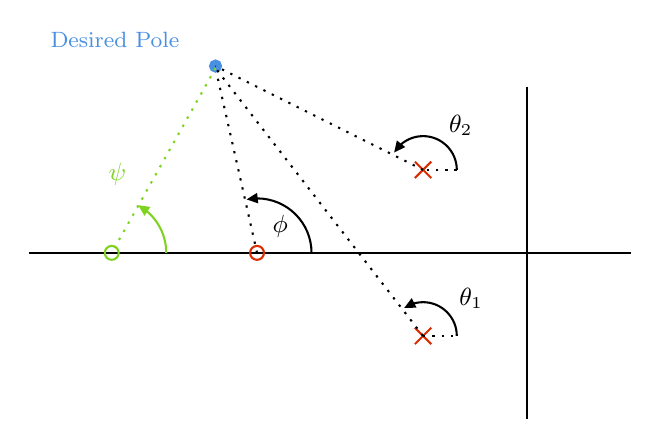
\begin{tikzpicture}[x=0.75pt,y=0.75pt,yscale=-1,xscale=1]
%uncomment if require: \path (0,300); %set diagram left start at 0, and has height of 300

%Straight Lines [id:da43586919548939607] 
\draw    (440,90) -- (440,250) ;
%Straight Lines [id:da9503958070649492] 
\draw    (490,170) -- (200,170) ;
%Straight Lines [id:da3241630090679538] 
\draw [color={rgb, 255:red, 218; green, 44; blue, 0 }  ,draw opacity=1 ]   (390,130) ;
\draw [shift={(390,130)}, rotate = 45] [color={rgb, 255:red, 218; green, 44; blue, 0 }  ,draw opacity=1 ][line width=0.75]    (-5.59,0) -- (5.59,0)(0,5.59) -- (0,-5.59)   ;
%Straight Lines [id:da5521431141710665] 
\draw [color={rgb, 255:red, 218; green, 44; blue, 0 }  ,draw opacity=1 ][line width=0.75]    (310,170) ;
\draw [shift={(310,170)}, rotate = 0] [color={rgb, 255:red, 218; green, 44; blue, 0 }  ,draw opacity=1 ][line width=0.75]      (0, 0) circle [x radius= 3.35, y radius= 3.35]   ;
%Straight Lines [id:da7608033603021352] 
\draw [color={rgb, 255:red, 218; green, 44; blue, 0 }  ,draw opacity=1 ]   (390,210) ;
\draw [shift={(390,210)}, rotate = 45] [color={rgb, 255:red, 218; green, 44; blue, 0 }  ,draw opacity=1 ][line width=0.75]    (-5.59,0) -- (5.59,0)(0,5.59) -- (0,-5.59)   ;
%Straight Lines [id:da5699006080990305] 
\draw  [dash pattern={on 0.84pt off 2.51pt}]  (310,170) -- (290,81) ;
%Shape: Arc [id:dp5285449429163444] 
\draw  [draw opacity=0] (304.99,144.23) .. controls (306.61,143.91) and (308.29,143.75) .. (310,143.75) .. controls (324.5,143.75) and (336.25,155.5) .. (336.25,170) -- (310,170) -- cycle ; \draw    (307.96,143.83) .. controls (308.64,143.78) and (309.31,143.75) .. (310,143.75) .. controls (324.5,143.75) and (336.25,155.5) .. (336.25,170) ;  \draw [shift={(304.99,144.23)}, rotate = 353.48] [fill={rgb, 255:red, 0; green, 0; blue, 0 }  ][line width=0.08]  [draw opacity=0] (5.36,-2.57) -- (0,0) -- (5.36,2.57) -- cycle    ;
%Straight Lines [id:da15323176218116707] 
\draw  [dash pattern={on 0.84pt off 2.51pt}]  (390,210) -- (406.25,210) ;
%Shape: Arc [id:dp08912661566072977] 
\draw  [draw opacity=0] (380.91,196.53) .. controls (383.51,194.77) and (386.63,193.75) .. (390,193.75) .. controls (398.97,193.75) and (406.25,201.03) .. (406.25,210) -- (390,210) -- cycle ; \draw    (383.56,195.08) .. controls (385.53,194.22) and (387.71,193.75) .. (390,193.75) .. controls (398.97,193.75) and (406.25,201.03) .. (406.25,210) ;  \draw [shift={(380.91,196.53)}, rotate = 333.09] [fill={rgb, 255:red, 0; green, 0; blue, 0 }  ][line width=0.08]  [draw opacity=0] (5.36,-2.57) -- (0,0) -- (5.36,2.57) -- cycle    ;
%Shape: Arc [id:dp6201158238747911] 
\draw  [draw opacity=0] (376.07,121.63) .. controls (378.91,116.91) and (384.09,113.75) .. (390,113.75) .. controls (398.97,113.75) and (406.25,121.03) .. (406.25,130) -- (390,130) -- cycle ; \draw    (377.88,119.18) .. controls (380.85,115.85) and (385.18,113.75) .. (390,113.75) .. controls (398.97,113.75) and (406.25,121.03) .. (406.25,130) ;  \draw [shift={(376.07,121.63)}, rotate = 308.31] [fill={rgb, 255:red, 0; green, 0; blue, 0 }  ][line width=0.08]  [draw opacity=0] (5.36,-2.57) -- (0,0) -- (5.36,2.57) -- cycle    ;
%Straight Lines [id:da2415895366325257] 
\draw  [dash pattern={on 0.84pt off 2.51pt}]  (406.25,130) -- (390,130) ;
%Straight Lines [id:da7442727174623508] 
\draw [color={rgb, 255:red, 74; green, 144; blue, 226 }  ,draw opacity=1 ]   (290,81) -- (290,80) ;
\draw [shift={(290,80)}, rotate = 270] [color={rgb, 255:red, 74; green, 144; blue, 226 }  ,draw opacity=1 ][fill={rgb, 255:red, 74; green, 144; blue, 226 }  ,fill opacity=1 ][line width=0.75]      (0, 0) circle [x radius= 2.68, y radius= 2.68]   ;
%Straight Lines [id:da4779442127163923] 
\draw  [dash pattern={on 0.84pt off 2.51pt}]  (390,210) -- (290,81) ;
%Straight Lines [id:da9872910863944787] 
\draw  [dash pattern={on 0.84pt off 2.51pt}]  (390,130) -- (290,80) ;
%Straight Lines [id:da1478915278912486] 
\draw [color={rgb, 255:red, 126; green, 211; blue, 33 }  ,draw opacity=1 ][line width=0.75]    (240,170) ;
\draw [shift={(240,170)}, rotate = 0] [color={rgb, 255:red, 126; green, 211; blue, 33 }  ,draw opacity=1 ][line width=0.75]      (0, 0) circle [x radius= 3.35, y radius= 3.35]   ;
%Straight Lines [id:da9672819226845463] 
\draw [color={rgb, 255:red, 126; green, 211; blue, 33 }  ,draw opacity=1 ] [dash pattern={on 0.84pt off 2.51pt}]  (290,81) -- (240,170) ;
%Shape: Arc [id:dp9522949619064215] 
\draw  [draw opacity=0] (252.73,147.04) .. controls (260.79,151.52) and (266.25,160.12) .. (266.25,170) -- (240,170) -- cycle ; \draw [color={rgb, 255:red, 126; green, 211; blue, 33 }  ,draw opacity=1 ]   (255.29,148.66) .. controls (261.93,153.43) and (266.25,161.21) .. (266.25,170) ;  \draw [shift={(252.73,147.04)}, rotate = 33.57] [fill={rgb, 255:red, 126; green, 211; blue, 33 }  ,fill opacity=1 ][line width=0.08]  [draw opacity=0] (5.36,-2.57) -- (0,0) -- (5.36,2.57) -- cycle    ;

% Text Node
\draw (316,150.4) node [anchor=north west][inner sep=0.75pt]  [font=\small]  {$\phi $};
% Text Node
\draw (406,185.4) node [anchor=north west][inner sep=0.75pt]  [font=\small]  {$\theta _{1}$};
% Text Node
\draw (401,102.4) node [anchor=north west][inner sep=0.75pt]  [font=\small]  {$\theta _{2}$};
% Text Node
\draw (209,62) node [anchor=north west][inner sep=0.75pt]  [color={rgb, 255:red, 74; green, 144; blue, 226 }  ,opacity=1 ] [align=left] {{\footnotesize Desired Pole}};
% Text Node
\draw (237,125.4) node [anchor=north west][inner sep=0.75pt]  [font=\small,color={rgb, 255:red, 126; green, 211; blue, 33 }  ,opacity=1 ]  {$\psi $};


\end{tikzpicture}

    \caption{Introduction of a new pole to meet angle condition}
    \label{fig:pid zero}
\end{figure}
We can write the appropriate equation for the angle deficiency as:
$$\sum\phi_i-\sum\theta_j+\psi=180\degree$$
Here, $\phi$ and $\theta$ are the angles from the desired pole of the system to the other poles and zeros of the system, as in $\angle(s_d-p_i)$. To meet this condition, we use the PD controller. If the angle deficiency required is positive, we can add a zero to the system with:
$$K_{PD}(s)=K_c(s+z_c)$$
Otherwise, we actually need to introduce a pole to the system to provide negative phase. This does not happen often, as it signifies that our transient response is better than desired. In that case, we would often just do nothing. Nonetheless,  we could alter the system by using a controller like:
$$K(s)=K_c\frac{1}{s+p_c}$$
In either case, we can determine the necessary value of $z_c$ or $p_c$ from the angle condition. Then we can determine the value of $K_c$ using the magnitude condition.

\begin{example}[PD control design example]
Consider we desire a system with closed loop poles at $s_d=-2\pm2\sqrt{3}i$ and our uncompensated system has the loop transfer function:
$$G(s)=\frac{4}{s(s+2)}$$
As a first step, we can calculate the angle deficiency of the system. Given the pole locations, we find that $\psi=30\degree$. We must add positive phase so we choose a standard PD controller design. To get a $30\degree$ angle, we must place the zero at $-8$. Then, we find the magnitude of the whole system:
$$\left|K_c\frac{4(s+8)}{s(s+2)}\right|_{s=s_d}=1$$
This condition let's us uniquely determine $K_c$, which we find is 1/2. The numbers are not always so clean, but we can use a calculator or computer software to help.
\end{example}

The next step is to design the integrator. For this system, we do not require one if our goal is to have zero steady state error to the step. However, we can include one to improve tracking response to a ramp input or other general inputs. The general form of the PI controller is:
$$K_{PI}(s)=K_c\frac{s+z_c}{s}$$
Here, the design is very simple. To ensure that the transient response of the system is not changed very much, we just place the zero close to the origin of the left half plane. A common choice is $z_c=0.05$ or $z_c=0.1$. Really, the choice is up to the engineer. Smaller values of $z_c$ will change the steady state response by a smaller amount, but values closer to zero can give a more sluggish reduction of steady state error. Small values can also make the controller less robust under design uncertainties.

To find $K_c$, we again use the magnitude condition. Let's choose $z_c=0.01$ and find the necessary $K_c$. If we designed the transient response already, we need not worry about including that in the calculation now, since it's magnitude is already 1 at the closed loop pole. Thus, we only need to analyze:
$$\left|K_c\frac{s+0.01}{s}\right|_{s=s_d}=1$$
For the choice of poles in our example, this gives us $K_c=1.007$. Altogether, our controller will be the combination of the PI and PD controllers. We simply multiply the two together to get the final PID controller:
$$K_{PID}=\frac{1}{2}(s+8)\cdot1.007\frac{s+0.01}{s}=\frac{0.5035s^2+4.033s+0.040}{s}$$

\subsection{Lead-Lag Compensators}
When we discussed the PID controller, there was one pretty apparent issue. The PID controller is not physically realizable, because the transfer function is improper! Implementing a true derivative in the filter is not practically possible. As a result, we sometimes choose to design a different type of controller which is more easily built for physical systems. Instead of including a pure derivative or integral in the system, lead-lag compensators lose some performance benefits (like zero steady state error) to create a more physically realizable controller.

The design methodology for lead-lag compensators is nearly identical to PID design. As a result, I will keep this section brief and the let the reader fill in the neccesary details. For lead-lag systems, the transfer function looks like:
$$K(s)=K_c\frac{s+z_c}{s+p_c}$$
If the system is a lead compensator (helps with transient response), then the value of $p_c$ is greater than the value of $z_c$. In a lag compensator, the opposite is true. I always get the two confused, but in design the choice will be apparent.

To design a transient response for the system, we follow the same steps that we would for the PD controller. If the phase deficiency is positive, we add a lead compensator. We choose the angle between the pole, zero, and desired pole to be the phase deficiency. We still have a degree of freedom here, but it is often wise to move the pair further rightward to make the system simpler in implementation. 

\todo{Insert figure of the lead phase here}

When trying to improve the steady state response, the ratio between $z_c$ and $p_c$ will dictate the reduction in the steady state error. Often, we choose to reduce it by a factor of $10$ or so, but this will depend on the specific needs for the system. We just need to remember:
$$\frac{z_c}{p_c}=\text{steady state error reduction factor}$$
Again, we like to place the zero fairly close to the origin in order to not change the transient response of the system much. These values can be chosen in a similar way to the PID controller. Once again, we then choose $K_c$ such that the magnitude condition is satisfied.

Together, these two methods allow us to design controllers using the root locus approach. While this design methodology is quite powerful, it does leave a few questions. For example, it does not give any notion of when our system might become unstable, or how the response of the system depends on the frequency of the input. For this type of insight, we must turn our attention to controller design in the frequency domain.


\newpage
\printendnotes
\chapter{Frequency Domain Design}\label{chap:frequency}
Transfer functions lend themselves quite readily to a description in the frequency domain. Using these relationships, we can understand the nature of a transfer function by understanding the response to different frequencies. This section will discuss the various methods by which this is done, and how they allow us to analyze systems. The most popular methodology is the Bode plot.

\section{Bode Plots}
The core idea behind the Bode plot is to understand how a transfer function behaves over the range of all frequencies, and plot that behavior. Before we can do that, however, we need more context about transfer functions.

One relationship of stable transfer functions that we have not mentioned yet is that when a sinusoid is input into the transfer function, the output at steady state must also be a sinusoid of the same frequency!
\begin{figure}[H]
    \centering
    \includesvg[width=0.75\linewidth]{Images/SinusoidInOut.svg}
    \caption{Sinusoid Input Output Relationship}
    \label{fig:sinInOut}
\end{figure}
We can see this quite readily by considering the operations that we can perform on a sine wave in a linear system. We can:
\begin{enumerate}
    \item Multiply by a constant, $a$
    \item Add or subtract another sine wave
    \item Integrate the sine wave
    \item Differentiate the sine wave
\end{enumerate}

The operations above are the only operations we can perform, because any other type of input will violate the zero-input zero-output quality of the transfer function and the system is therefore nonlinear. These operations, in effect, are the only operations that preserve linearity of the system.

More mathematically, we can consider a general system with transfer function $G(s)$. We require $G(s)$ to be stable for this result to be true, so we know that $G(s)$ must take the form:
$$G(s) = \frac{a_0+a_1s+a_2s^2+\dots}{(s+s_1)(s+s_2)\dots}$$
Supposing that each $s_n$ is positive, all poles lie in the LHP and the system is stable. Now, we multiply this transfer function by an input sine wave, $A\sin\omega t$. In the Laplace domain:
$$A\sin\omega t \overset{\mathscr{L}}{\rightarrow}\frac{A\omega}{s^2+\omega^2}$$
Multiplying the two terms together, we have:
$$G(s)\frac{A\omega}{s^2+\omega^2}=\frac{a}{s+i\omega}+\frac{\bar{a}}{s-i\omega}+$$
If you think carefully about this representation, you can convince yourself that any stable $G(s)$ may be represented this way. Try writing some simple examples to see. The big point is that applying any of these operations (or any combination of them) will yield another sine wave, with the only possible variation being the \textbf{phase} and \textbf{amplitude} of the wave.

\begin{example}[Addition of sine waves]
    Here, I will show one example with the addition of sine waves. We may start with two arbitrary waves, say:\begin{gather}
        \sin(2x)\\
        2\cos(2x)
    \end{gather}
    Importantly, these sine waves must have the same frequency, but the phase and the amplitude may be whatever we desire. We add these sine waves to get:
$$ \sin(2x)+2\cos(2x)$$
It is not obvious that this should give a sinusoidal output, but it can be shown that the result must be a sinusoid through the application of the following trigonometric identity:
$$a\sin x+b\cos x=\sqrt{a^2+b^2}\sin\left[x+\arctan\left(\frac{b}{a}\right)\right]$$
Applying this formula to our scenario, we see that the resulting sine wave is:
$$\sqrt{3}\sin(2x+1.107)$$
We can directly see that as a result of this addition, we get a new sine wave with the same frequency, but an additional gain and phase shift:
\[
\underbrace{\color{red}\sqrt{3}}_{\color{red}\text{gain}}\color{black}\sin\left(2x + \underbrace{\color{blue}1.107}_{\color{blue}\text{phase}}\color{black}\right)
\]
\end{example}
    The principle is indeed general. The gain is given as sum total of the sine wave amplitudes and the phase by the combination of all offset waves. These can always be described in terms of just two scalar values for gain and phase. Of course, the gain and phase will change as the input frequency of the sine waves changes! This fact is what makes the response of a system interesting.

\begin{exercise}
    Show that the other three identities must return a sine wave of the same frequency as a result. The remaining three identities are:
    \begin{enumerate}
        \item Multiplication by a constant
        \item Integration of a sine wave
        \item Differentiation of a sine wave
    \end{enumerate}

    Show that these properties hold for an arbitrary sine wave
\end{exercise}

We call the change in the amplitude of the input sine wave the gain, and the change in the phase is the phase shift. Often, we choose to express gain in terms of decibels. To convert a standard gain into decibels, we can use the following formula:
$$\textrm{dB}=20\log\frac{A}{A_0}$$
Or if we simply consider the gain $K$, the value in decibels is given as:
$$\textrm{dB}=20\log K$$
The $\log$ here is the base-10 logarithm. These logarithmic units are often used in audio applications because the response of the human ear is also close to logarithmic.\endnote{Interestingly, so is the response of the human eye to brightness. This is why astronomical magnitudes are also on a logarithmic scale.} These conventions transfer over to control theory applications, so it is necessary to understand the conversion. A negative dB value indicates that the gain is between 0 and 1 (reducing the original signal gain). A positive value indicates that the original signal is amplified.

Phase is normally given in either radians or degrees. The standard convention is that a negative phase means that the system response is lagging. That is to say, if we input a sine wave and the system is 20\degree behind the input wave, we have a phase shift of $-20\degree$.

That's about all the background we need to get started with frequency domain design. Since our systems are linear, if we understand how a few simple transfer functions look on the Bode plot, we can combine them together to create more complicated transfer functions. We'll now cover the basic transfer functions and what their Bode plots look like. After that, we can apply this analysis to any system which is given by a transfer function.

\subsection{Bode Plots of Standard Transfer Functions}

\subsubsection{Poles}

\subsubsection{Zeros}

\subsubsection{Second Order System Responses}

\subsection{General Bode Plots}

\subsection{Bode Plots with MATLAB}


\section{Gain and Phase Margin}


\section{Nyquist Plots}

\subsection{The Nyquist Stability Criterion}

\subsection{Disk Margin }

\section{Nichols Chart}


\newpage
\printendnotes

